% !Mode:: "TeX:UTF-8"
% 
% 编译说明
%		使用 XeLaTeX 编译引擎
%       TeX Live 的版本 2022 和 2021 目前都可以成功编译
%       如果使用 Overleaf 进行写作,请在左上角菜单中选择编译器为 XeLaTeX
%		在 MacBook 中推荐使用编译软件 Texpad


\documentclass[doctor]{bnuthesis}
	% bachelor/master/doctor: 学士/硕士/博士学位论文
	% twoside: 奇数页和偶数页页边距不一样,用于打印
	\usepackage{bnutils}
	% 调用宏包,使用 GB/T 7714-2015 参考文献著录格式
	\usepackage{gbt7714}
	
	% 添加脚注相关包
	% \usepackage{footnote}
	% \usepackage[perpage=false]{footmisc}
	
	% Override document class footnote system for continuous numbering
	\makeatletter
	% Disable per-page reset by redefining the footnote counter
	\newcounter{globalfootnote}
	\setcounter{globalfootnote}{0}
	\renewcommand{\thefootnote}{\arabic{globalfootnote}}
	\renewcommand{\thempfootnote}{\arabic{globalfootnote}}
	\makeatother
	
	% 确保natbib可用
	% \usepackage{natbib}
	% \usepackage{bibentry}
	% \nobibliography*
	
	% 自定义脚注引用命令
	% 命令:在脚注中显示完整的参考文献信息
	\newcommand{\footcite}[1]{\footnote{\bibentry{#1}}}
	
	% 命令:在脚注中显示完整的参考文献信息(带说明文字)
	\newcommand{\footcitewith}[2]{%
		\footnote{%
			#2 \cite{#1}%
		}%
	}
	
	% 命令:在脚注中显示多个参考文献
	\newcommand{\footcitemulti}[1]{%
		\footnote{%
			\cite{#1}%
		}%
	}
	
	\begin{document}
	\graphicspath{{figures/}}
	
	\frontmatter
	% !Mode:: "TeX:UTF-8"

\ctitle{越南高等教育外部质量保证体系研究}
\etitle{Research on External Quality Assurance System of Vietnamese Higher Education}


\makeatother

% 学士学位封面
% \cbuyuanxi{天文系} % 部院系
% \czhuanye{天文学} % 专业
% \cxuehao{201511160109} % 学号
% \cxueshengxingming{某某某} % 学生姓名
% \czhidaojiaoshi{某某} % 指导教师
% \czhidaojiaoshizhicheng{教授} % 指导教师职称
% \czhidaojiaoshidanwei{北京师范大学天文系} % 指导教师单位

% 博士(硕士)学位封面
\czuozhe{张氏越祯} % 作者
\cdaoshi{高益民\ 教授} % 导师
\cxibienianji{教育学部2019级} % 系别年级
\cxuehao{201939010022} % 学号
\cxuekezhuanye{比较教育学} % 学科专业
\cwanchengriqi{2025年7月} % 完成日期


% 中文摘要
\begin{cabstract}
本论文系统研究了越南高等教育外部质量保障体系在快速扩张、国际化和问责要求不断提高背景下的转型与挑战。研究背景源于越南高等教育在过去二十年间的迅猛发展:从2000年的约200所高校、100万学生,发展到2023年的近500所高校、超过250万学生。这种规模扩张在带来机遇的同时,也带来了质量保障的严峻挑战,特别是在确保教育质量与数量增长同步、满足劳动力市场需求、以及应对国际竞争压力等方面。

通过全面梳理全球与区域发展趋势,论文揭示了推动外部质量保障(EQA)机制发展的主要动力,特别是在东盟区域内。研究发现,全球高等教育质量保障呈现出从单一合规导向向多元化、适应性模式转变的趋势。传统的以政府主导、标准化评估为主的质量保障模式正在被更加灵活、注重持续改进和利益相关者参与的混合模式所替代。在东盟地区,这种趋势表现得尤为明显,各国在保持本土特色的同时,也在积极寻求区域合作与标准协调。

研究采用定性比较案例研究方法,深入分析了越南EQA体系的现状、成就与挑战。通过对越南教育部质量保障政策文件、评估报告和专家访谈的系统分析,研究识别出越南EQA体系在制度建设、评估机制、国际合作等方面的主要成就。同时,研究也揭示了体系存在的关键问题,包括评估标准不够细化、评估专家队伍能力不足、评估结果应用不充分、以及利益相关者参与度不高等。

为了提供更全面的分析视角,研究借鉴了中国国家主导模式和东盟大学联盟质量保障(AUN-QA)框架的经验。中国案例展示了国家强力主导的质量保障体系在实现大规模、快速变革方面的优势,但也凸显了如何在严格控制与学术创新自主权之间取得平衡的挑战。AUN-QA案例则体现了基于合作、共识和同行网络的区域质量保障模式的力量,证明了在多样化环境中无需单一权力机构集中控制也能建立共同标准。

论文运用现代管理与组织理论,包括新制度主义、利益相关者理论和委托代理理论,构建了适合越南国情的V-AQA混合与适应性模型。该模型基于五个核心要素构建:(1)领导与治理,强调战略导向和有效治理结构;(2)质量文化,注重建立持续改进的组织文化;(3)利益相关者参与,确保多方利益的有效整合;(4)内部流程,建立系统化的质量保障机制;(5)合作与协调,促进内部协作和外部合作。这五个要素相互关联、动态互动,形成了一个完整的质量保障生态系统。

研究结果指出,越南高等教育在规模扩张、资源分配和人才培养与劳动力市场需求之间仍面临诸多挑战。具体表现在:教育质量与数量增长不同步,优质教育资源分布不均,人才培养与就业市场需求脱节,以及国际竞争力有待提升等方面。这些挑战的根源在于质量保障体系的不完善,特别是在评估标准、专家队伍、结果应用和利益相关者参与等方面存在不足。

基于理论分析和国际比较,论文最终提出了以领导力、质量文化、利益相关方参与、内部流程和合作为核心的EQA体系综合改革模型。该模型强调:(1)建立多层次、协调统一的质量保障治理体系;(2)培育以质量为核心的组织文化;(3)构建多元利益相关者参与机制;(4)完善系统化的内部质量保障流程;(5)加强国内协作和国际合作。这一改革模型旨在提升体系效能,促进质量持续改进,助力越南高等教育更好地融入区域与全球教育体系。

研究的理论贡献在于构建了适合发展中国家高等教育质量保障的分析框架,丰富了质量保障理论在转型国家背景下的应用。实践意义在于为越南高等教育质量保障体系改革提供了系统性的政策建议,同时也为其他类似背景的国家提供了有价值的参考。研究结论强调,有效的质量保障体系不仅是一套流程的集合,而是一个复杂的生态系统,需要领导力、文化、利益相关者、流程和合作之间的动态平衡。
\end{cabstract}
\ckeywords{质量保障;高等教育;越南;外部质量保障;改革模型}

% English abstract
\begin{eabstract}
This dissertation investigates the transformation and challenges of Vietnam's higher education quality assurance system in the context of rapid expansion, international integration, and increasing demands for accountability. The research background stems from Vietnam's remarkable higher education development over the past two decades: from approximately 200 institutions and 1 million students in 2000 to nearly 500 institutions and over 2.5 million students in 2023. While this scale expansion has brought opportunities, it has also created serious quality assurance challenges, particularly in ensuring synchronized quality and quantity growth, meeting labor market demands, and responding to international competitive pressures.

Through a comprehensive review of global and regional trends, the study identifies the driving forces behind the development of external quality assurance (EQA) mechanisms, particularly in the ASEAN region. The research reveals that global higher education quality assurance is transitioning from single compliance-oriented approaches to diversified, adaptive models. Traditional government-led, standardized assessment quality assurance models are being replaced by more flexible approaches that emphasize continuous improvement and stakeholder engagement. This trend is particularly evident in the ASEAN region, where countries maintain their local characteristics while actively seeking regional cooperation and standard harmonization.

Using a qualitative comparative case study design, the research analyzes Vietnam's EQA system in depth, examining its current status, achievements, and challenges. Through systematic analysis of Vietnam's Ministry of Education quality assurance policy documents, evaluation reports, and expert interviews, the study identifies major achievements in Vietnam's EQA system regarding institutional development, evaluation mechanisms, and international cooperation. Simultaneously, the research reveals critical issues within the system, including insufficiently detailed evaluation standards, inadequate capacity of evaluation expert teams, insufficient application of evaluation results, and low stakeholder participation levels.

To provide a more comprehensive analytical perspective, the study draws lessons from China's state-driven model and the ASEAN University Network Quality Assurance (AUN-QA) framework. The China case demonstrates the advantages of a state-dominated quality assurance system in achieving large-scale, rapid transformation, but also highlights the challenge of balancing strict control with academic innovation autonomy. The AUN-QA case exemplifies the power of a regional quality assurance model based on cooperation, consensus, and peer networks, proving that common standards can be established in diverse environments without centralized control by a single authority.

The study applies modern management and organizational theories—including new institutionalism, stakeholder theory, and principal-agent theory—to construct the V-AQA hybrid and adaptive model, tailored to Vietnam's unique context. This model is built on five core elements: (1) Leadership and Governance, emphasizing strategic orientation and effective governance structures; (2) Quality Culture, focusing on establishing continuous improvement organizational culture; (3) Stakeholder Engagement, ensuring effective integration of multiple interests; (4) Internal Processes, establishing systematic quality assurance mechanisms; and (5) Cooperation and Coordination, promoting internal collaboration and external cooperation. These five elements are interconnected and dynamically interactive, forming a complete quality assurance ecosystem.

Findings highlight both achievements and persistent challenges, such as rapid scale growth, uneven resource distribution, and the gap between training outcomes and labor market needs. Specific manifestations include: asynchronous quality and quantity growth in education, uneven distribution of quality educational resources, disconnection between talent cultivation and employment market demands, and room for improvement in international competitiveness. The root causes of these challenges lie in the imperfection of the quality assurance system, particularly in areas such as evaluation standards, expert teams, result application, and stakeholder participation.

Based on theoretical analysis and international comparison, the dissertation concludes by proposing a comprehensive reform model for Vietnam's EQA system, emphasizing leadership, quality culture, stakeholder engagement, internal processes, and cooperation. This model emphasizes: (1) establishing a multi-level, coordinated quality assurance governance system; (2) cultivating quality-centered organizational culture; (3) constructing multi-stakeholder participation mechanisms; (4) perfecting systematic internal quality assurance processes; and (5) strengthening domestic collaboration and international cooperation. This reform model aims to enhance the system's effectiveness, support sustainable quality improvement, and facilitate Vietnam's integration into the regional and global higher education landscape.

The theoretical contribution of this research lies in constructing an analytical framework suitable for higher education quality assurance in developing countries, enriching the application of quality assurance theory in the context of transitional countries. The practical significance lies in providing systematic policy recommendations for Vietnam's higher education quality assurance system reform, while also offering valuable references for other countries with similar backgrounds. The research conclusion emphasizes that an effective quality assurance system is not merely a collection of processes, but a complex ecosystem requiring dynamic balance among leadership, culture, stakeholders, processes, and cooperation.
\end{eabstract}
\ekeywords{quality assurance; higher education; Vietnam; external quality assurance; reform model}



	\makecover
	
	\tableofcontents
	\listoffigures % 插图索引
	\listoftables % 表格索引
	
	\mainmatter
	\chapter{引言}
\label{chap:gioi_thieu}

\section{研究背景与选题理由}
\label{sec:boi_canh_ly_do}

\subsection{全球背景:质量保障成为必然趋势}

进入21世纪,高等教育(GDĐH)已超越其作为知识保存与传播场所的传统角色,成为决定各国竞争力和可持续发展的战略驱动力\footcite{Altbach2001}。在基于知识的全球化经济(knowledge-based economy)背景下,大学被视为"创新引擎",是培养高素质人力资源、产出科学技术发明以及为社会复杂挑战提供解决方案的场所\footcite{OECD_HE2008}。这一角色的转变对高等教育体系的质量提出了前所未有的紧迫要求。质量不再是学术象牙塔中的抽象概念,而已成为一个可衡量、可比较的因素,是国际舞台上激烈竞争的标准。

正是在这样的背景下,质量保障体系(ĐBCL - Quality Assurance),特别是外部质量保障(External Quality Assurance - EQA),已成为不可逆转的全球趋势。根据世界银行(World Bank)和联合国教科文组织(UNESCO)的报告,在过去几十年里,建立国家级质量保障机构的国家数量急剧增加,覆盖了全球几乎所有地区\footcite{WorldBank_QA_GlobalTrends}。这一强劲的扩散势头主要由三大动力推动:

\begin{enumerate}
    \item \textbf{高等教育的大众化 (Massification of Higher Education):} 学生规模和大学数量的爆炸性增长,包括私立院校的迅猛发展,使得高等教育体系变得前所未有的多样化和复杂化。这种多样性虽然带来了更多的教育机会,但同时也带来了质量下降和不均衡的风险。因此,政府和社会需要一个外部监督机制,以确保整个体系的最低质量门槛\footcite{Trow2007}。
    
    \item \textbf{问责制要求的提高 (Increased Demand for Accountability):} 随着公共财政和学习者对高等教育投入的日益增加,对大学问责制的要求也越来越高。包括政府、家长、学生和雇主在内的各利益相关方都想知道他们的投资是否带来了应有的效益。外部质量保障体系及其认证活动和结果公开,是履行这一问责制的最重要工具\footcite{Harvey2005}。
    
    \item \textbf{跨境教育的兴起 (Rise of Cross-border Education):} 全球化极大地促进了学生、教师和教育项目跨越国界的流动。这产生了对学位和学分互认的迫切需求。一个可靠的、其标准与国际惯例接轨的质量保障体系,是一个国家参与全球教育市场、吸引国际学生并确保本国学生文凭在国外获得承认的先决条件\footcite{Knight2006}。
\end{enumerate}

这些动力已将质量保障从一项纯粹的专业活动转变为一项重要的国家治理工具,是现代高等教育体系结构中不可或缺的要素。清晰理解这些全球趋势和动力,是准确分析像越南这样的特定国家质量保障体系所面临的背景与挑战的第一步。

\subsection{区域背景:东盟共同体内的质量协调化}
\label{subsec:boi_canh_khu_vuc}

如果说全球背景带来了竞争与融合的压力,那么区域背景则提出了合作与协调的要求。对越南而言,最重要的区域背景是东盟共同体。2015年东盟经济共同体(AEC)的成立设定了一个宏伟目标:建立一个统一的市场和生产基地,允许商品、服务、投资、资本以及特别是技术劳工(skilled labor)的自由流动\footcite{ASEAN_AEC_Blueprint}。

为实现这一目标,教育水平与质量的协调化及互认成为一项核心要求。在河内接受培训的工程师,需要具备与在曼谷或吉隆坡的雇主所承认的同等能力和文凭。深刻认识到这一要求,区域内的教育领导者们已率先努力建设一个共同的高等教育空间。实现这一努力最重要的工具是东盟大学网络(ASEAN University Network - AUN),特别是其下属的质量保障网络——AUN-QA(ASEAN University Network - Quality Assurance),该网络成立于1998年\footcite{AUNQA_History}。

AUN-QA并非一个具有强制权力的超国家认证机构,而是一个基于自愿、合作和同行学习(peer learning)原则运作的网络。其使命如官方文件所述,是"推动东盟高等教育机构的质量保障,提升高等教育质量,并为东盟共同体的共同利益与区域及国际机构合作"\footcite{AUN-QAGuide}。

AUN-QA的运作理念可概括为\textbf{"多元中的和谐"}原则。该网络不寻求消除各国教育体系之间的差异,而是建立一套共同的标准和评估流程,作为质量的"公分母"和通用语言。AUN-QA标准(目前是针对课程层级的4.0版)包含8项标准和明确的子标准,已成为该地区大学的重要参考框架。同行评审(peer review)流程,即由成员大学的专家相互评估,不仅有助于确保客观性,还创造了一个极其有效的经验和最佳实践分享机制\footcite{AUNQA_Report2023}。

对越南而言,积极参与AUN-QA网络具有战略意义。这不仅是提升国内大学质量和声誉的渠道,也是融入区域高等教育空间最快、最有效的途径。一个教育项目获得AUN-QA认证是其质量的重要保证,有助于该项目的毕业生在东盟劳动力市场上获得更多优势。因此,任何关于越南质量保障体系的分析都不能忽视AUN-QA框架作为区域背景重要因素的角色和影响。


\subsection{2015-2024年阶段越南高等教育发展背景:现状分析}

2015-2024年阶段标志着越南高等教育体系的一个重要转型时期。该体系已从注重扩大规模以满足社会学习需求,逐渐转向优先提升质量、调整结构和国际融合。分析此阶段的官方统计数据,将提供一幅全景图,突显越南高等教育所取得的成就、发展趋势以及面临的挑战,从而明确一个有效的外部质量保障体系产生的背景及其紧迫性。

\subsubsection{系统规模与结构的发展}

过去十年,越南高等教育最显著的特点之一是培养规模的急剧增长,而教育机构数量则在有控制地增长,体现了国家的战略导向。

\paragraph{关于教育机构数量:}
大学体系实现了稳定和可持续的发展。2015年,全国共有214所高等教育机构\footcite{stat_quy_mo_2015_2021},到2024年,这一数字增至\textbf{243所},其中包括176所公立大学和67所私立大学\footcite{stat_moet_2024}。近十年间仅净增约29所学校,表明政策不鼓励大规模新建学校,而是侧重于巩固和提升现有机构的质量。这为在整个体系内进行管理和质量保障工作创造了更有利的环境。

\paragraph{关于学生规模:}
与学校数量的稳定增长相反,学生规模实现了飞跃。大学生总规模从2015年的\textbf{175.3万}人猛增至2024年的\textbf{235.6万}人\footcite{stat_quy_mo_2015_2021}。这表明社会对大学学习的需求日益增长,高等教育体系已努力满足这一需求。

\begin{figure}
    \centering
    % Placeholder for the chart. Replace with your actual chart image.
    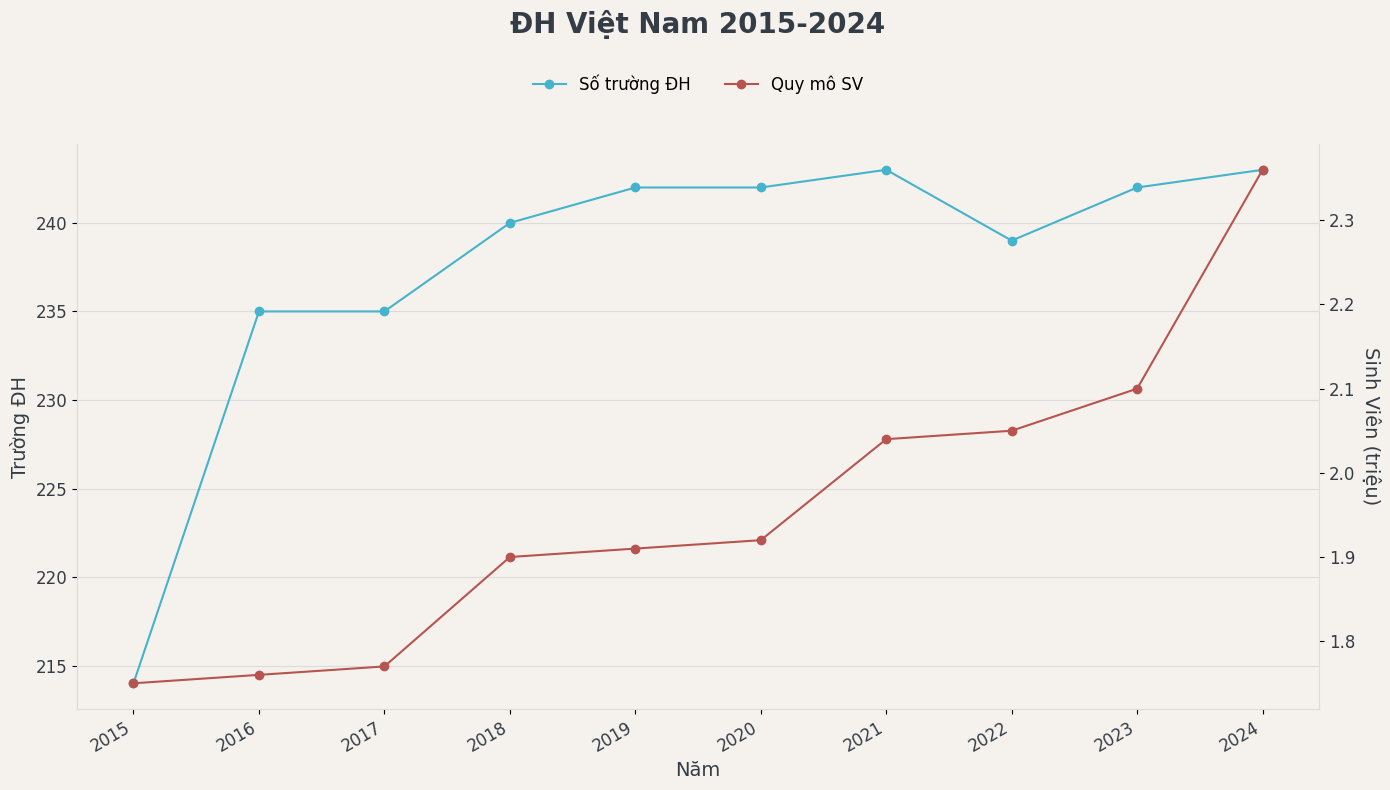
\includegraphics[width=0.9\textwidth]{image/bieu do 1 luan giao duc.png} 
    \caption{越南大学生规模与高校数量增长情况(2015-2024年)}
    \label{fig:quy_mo_phat_trien}
    \vspace{0.2cm}
    \footnotesize{\textit{来源:综合整理自越南教育培训部的数据\footcite{stat_moet_2024}及相关报告\footcite{stat_quy_mo_2015_2021}。}}
\end{figure}

特别是,2023-2024学年实现了突破性增长,比上一学年增加了\textbf{319,022}名学生\footcite{stat_moet_2024}。这并非寻常的线性增长,而是一次规模上的\textbf{飞跃(leap)},如图(图\ref{fig:quy_mo_phat_trien})所示。这种突增并非偶然现象,可以解释为多种政策和社会因素同时汇聚的结果,为整个体系带来了"推力"。

\paragraph{潜在原因分析:}
最直接和最重要的原因之一可能是各大学\textbf{招生政策的变化和招生指标的增加}。这一时期,除了传统的基于高中毕业考试成绩的录取方式外,多样化的录取方式也得到了大力发展。各大学加强使用学业成绩审查、自主能力评估考试等方式,为考生开辟了更多的"大门"。当大学,特别是民办大学和自主办学的公立大学,在确定招生指标和录取方式方面被赋予更多自主权时,它们倾向于扩大规模以满足社会需求和优化资源。整个体系招生指标的增加,结合灵活的录取方式,为前所未有的大量考生被录取和入学创造了条件。

第二个原因来自\textbf{经济社会因素和观念的转变}。COVID-19疫情后时期(2020-2022年)对劳动力市场和职业选择产生了一定影响。可能有一大部分学生和家庭意识到,对于没有高等专业水平的人来说,劳动力市场存在不确定性,从而坚定了大学文凭是未来稳定生活的必要"保险单"的信念。社会观念中"普及大学教育"的压力,推动了更大部分高中毕业生决定追求更高层次的学术道路,而不是进入劳动力市场或其他职业教育体系。

最后,这种突增是\textbf{共振效应}的结果。越南教育培训部扩大招生自主权的政策,如同一个"泄压阀",释放了社会长期以来积累的"需求压力"。当大学之门比以往任何时候都更加敞开时,大量的社会学习愿望在同一个学年得以实现,从而造成了规模上的飞跃。

然而,规模的快速增长也正是对质量保障工作的最大挑战。它提出了一个紧迫的问题:师资队伍、物质设施,特别是内部质量管理流程的发展,是否能跟上学生数量的增长速度?这正是现实背景,要求一个外部质量保障体系必须有效运作,既能监督,又能支持各大学克服这一挑战。

\paragraph{关于学生结构与民办院校的角色:}
民办大学的发展是教育社会化的一个亮点。就读于民办学校的学生比例已逐渐增加,从2015年的约20\%上升到2024年的\textbf{22.76\%},学生人数达到536,295人\footcite{stat_moet_2024}。这一数字不仅显示了私营部门日益重要的贡献,也表明越南已**提前实现了政府第35号决议中提出的到2025年民办学生比例达到22.5\%的目标**。民办院校的壮大创造了一个良性竞争的环境,推动公立学校不断创新和提高质量。

\subsubsection{招生工作现状与专业选择趋势分析}

分析招生数据不仅能展现体系的输入端情况,还能反映年轻一代的职业选择趋势,这是质量保障体系需要掌握并作出相应调整的重要因素。

\paragraph{参与比例与招生结果:}
近年来,参加高中毕业考试的考生数量一直稳定在100万以上\footcite{stat_thi_sinh_2024}。值得注意的是,申请大学录取的考生比例占了很大一部分,2024年约占参考考生总数的\textbf{68.5\%},显示进入大学仍然是大多数学生的首选。

被录取后确认入学的考生比例是反映培养项目吸引力和契合度的重要指标。在2022年短暂下降(80.34\%)后,该比例已恢复并于2024年达到\textbf{81.87\%},共有551,497名考生确认入学\footcite{stat_nhap_hoc_2024}。

% --- CHÈN BIỂU ĐỒ 2 ---
% --- CHÈN BIỂU ĐỒ (PHIÊN BẢN ĐÃ CẬP NHẬT) ---
\begin{figure}[h!]
    \centering
    % Thay thế bằng tên file ảnh mới bạn vừa tạo bằng Python
    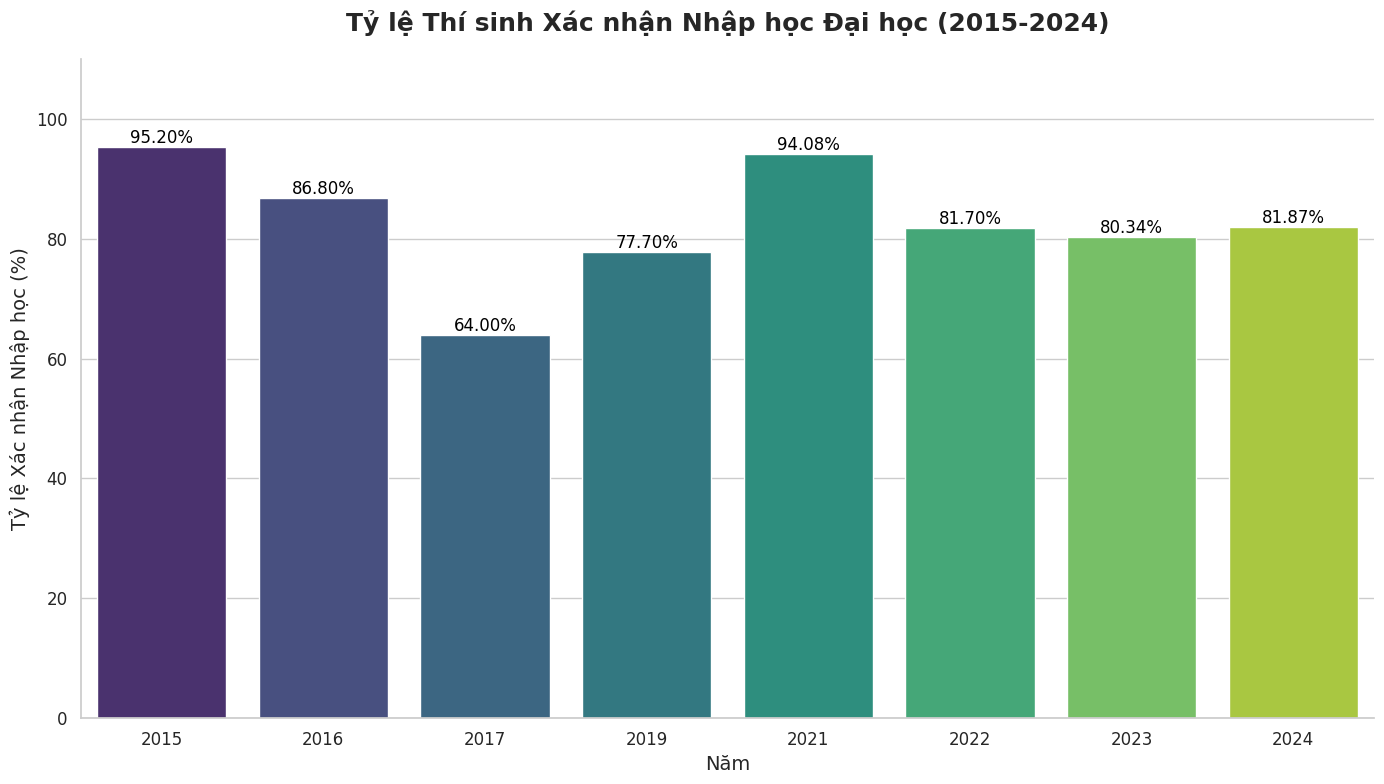
\includegraphics[width=0.8\textwidth]{image/ty_le_nhap_hoc_2015-2024.png}
    
    % Cập nhật caption cho đúng giai đoạn
    \caption{大学新生确认入学比例(2015-2024年)}
    \label{fig:ty_le_nhap_hoc_full}
    \vspace{0.2cm}
    
    % Cập nhật dòng nguồn với đầy đủ các trích dẫn
    \footnotesize{\textit{来源:综合整理自越南教育培训部及各新闻媒体历年数据 
    \footcite{ref1}\footcite{ref2}\footcite{ref3}\footcite{ref5}\footcite{ref7}\footcite{ref12}\footcite{ref19}\footcite{stat_nhap_hoc_2024}。}}
\end{figure}

这表明社会对高等教育体系的信心正在得到巩固。高入学率也意味着,平均每100名参加高中毕业考试的学生中,约有53人进入大学,这是过去9年来的最高比例,证实了越南已真正进入高等教育大众化阶段\footcite{stat_ty_le_vao_dh_2023}。

\paragraph{专业选择趋势:}
2024年的招生申请数据显示,专业选择趋势发生了显著变化。**教育科学与教师培养**类专业的志愿数量出人意料地大幅增长,比2023年增加了\textbf{85\%}。自然科学领域也吸引了大量关注,增幅达61\%\footcite{stat_tuyen_sinh_2024_so_lieu}。

相反,前些年的"热门"专业如**工商管理**(-3\%)和**计算机与信息技术**(-5\%)则出现了小幅下降趋势\footcite{stat_tuyen_sinh_2024_so_lieu}。这一转变可能反映了社会对长期人力资源需求的认知变化以及国家对教育行业的新政策。这是一个重要的信号,质量保障机构和各大学需要深入分析,以便及时调整培养结构。

\subsubsection{资源分析:师资队伍与物质设施}

一个教育体系的质量在很大程度上取决于其师资队伍的质量和保障条件。

\paragraph{关于师资队伍:}
2023-2024学年,全系统共有\textbf{88,031名全职教师}。在学历方面,有\textbf{28,862名教师拥有博士学位(占32.8\%)},49,229名教师拥有硕士学位(占55.9\%),其余为本科学历或其他学历\footcite{stat_moet_2024}。该学历结构如图\ref{fig:co_cau_giang_vien}所示。拥有博士学位的教师比例与前几年相比有了显著提高,这是提升培养和研究质量的重要前提。


% --- CHÈN BIỂU ĐỒ 3 ---
\begin{figure}[h!]
    \centering
    % Placeholder for the chart. Replace with your actual chart image.
    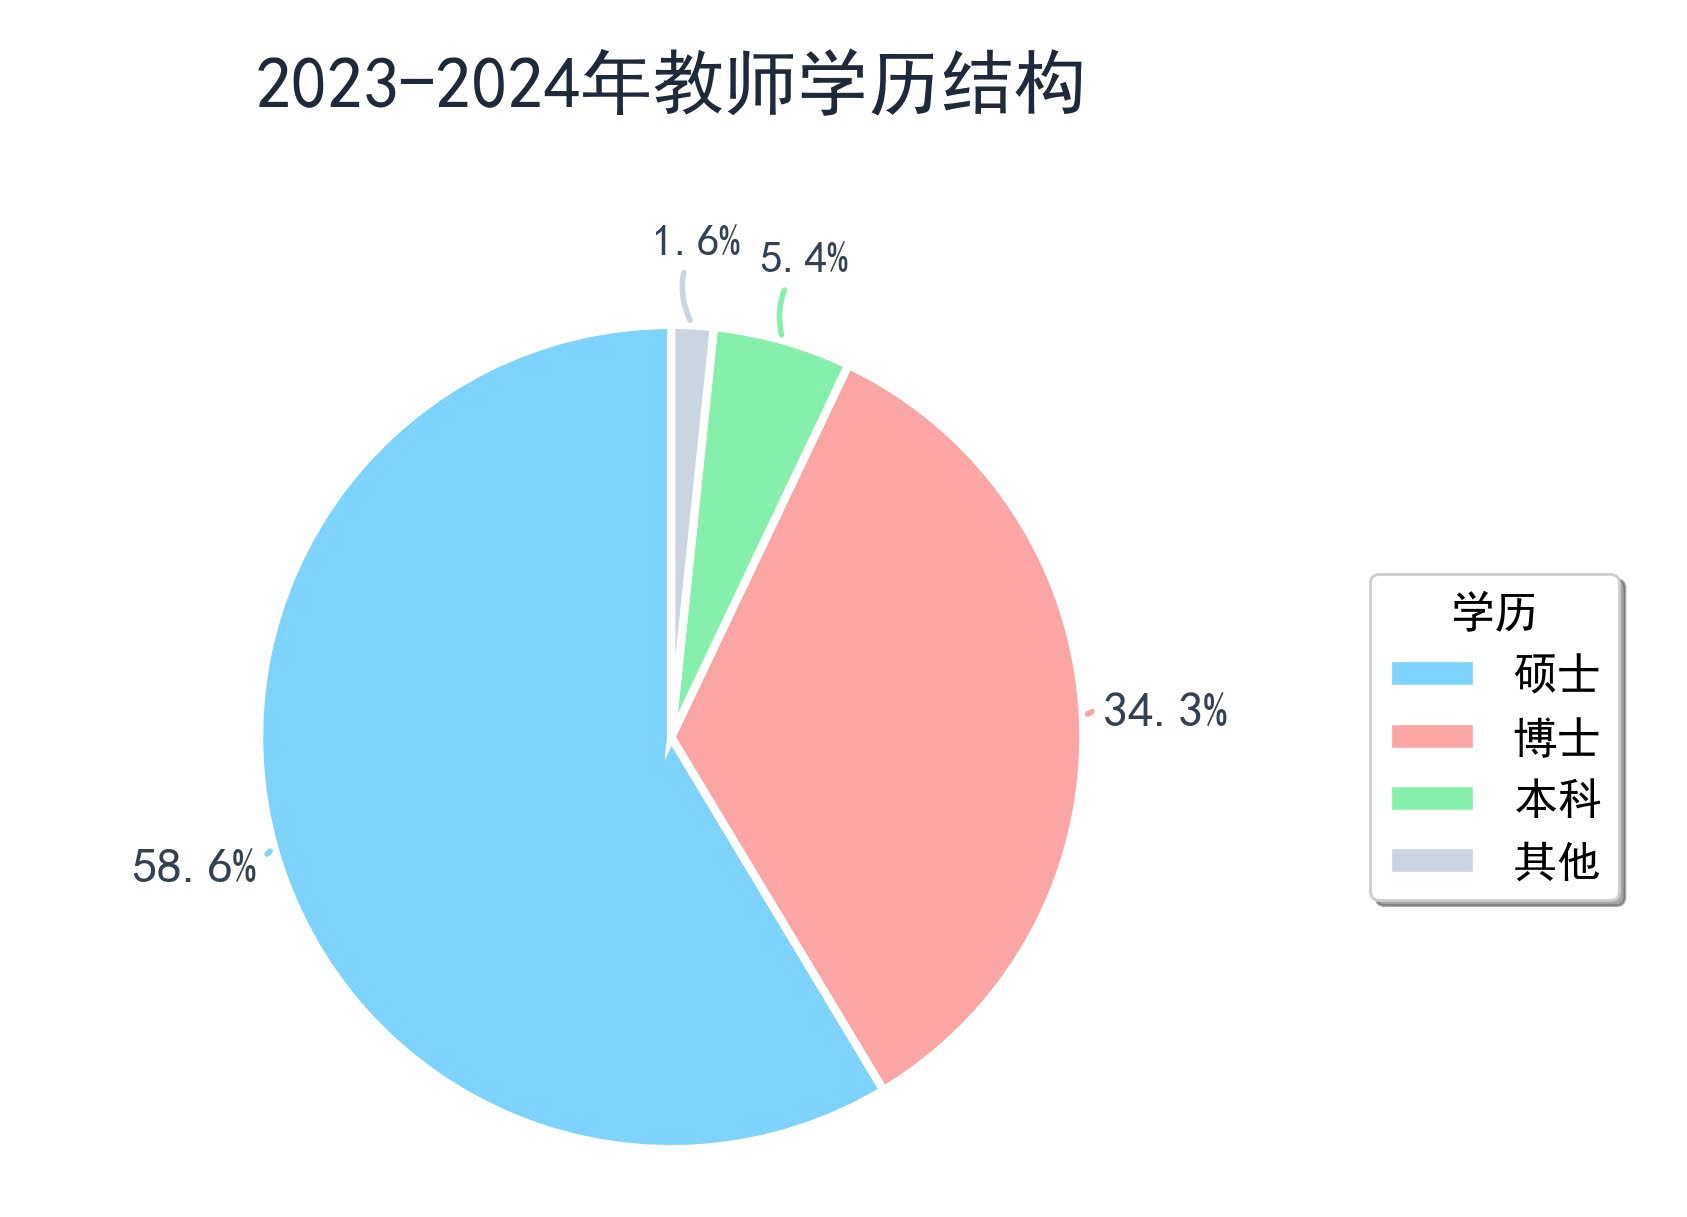
\includegraphics[width=0.6\textwidth]{image/co_cau_trinh_do_giang_vien_2023_2024.jpg}
    \caption{2023-2024学年全职教师学历结构}
    \label{fig:co_cau_giang_vien}
    \vspace{0.2cm}
    \footnotesize{\textit{来源:根据越南教育培训部数据计算\footcite{stat_moet_2024}。}}
\end{figure}

然而,生师比仍然偏高,尤其是在公立大学。全国平均生师比为公立大学30:1,民办大学22:1\footcite{stat_moet_2024}。公立大学的高生师比对确保师生之间有效互动(教育质量的核心要素)提出了巨大挑战。

\paragraph{关于资源分布:}
体系一个巨大且固有的挑战是地理分布上的严重不均衡。高质量的大学和师资队伍主要集中在红河三角洲(占学校总数的44.3\%)和东南部(18.4\%)两大重点经济区。而西原等贫困地区仅占学校总数的1.6\%\footcite{stat_quy_mo_2015_2021}。这种不平衡也明显体现在接受高等教育的机会上,红河三角洲的学生升入大学的比例(64.44\%)显著高于中北部山区(40.25\%)\footcite{stat_ty_le_vao_dh_2023}。这种差距要求质量保障政策必须考虑到地区因素,以确保公平和均衡发展。

\subsubsection{产出分析:毕业与就业}

产出质量是一个教育体系最终和最重要的衡量标准。
\begin{itemize}
    \item \textbf{毕业数量:} 2024年,高等教育体系为劳动力市场提供了\textbf{313,572名学士、工程师},与2023年的228,092人相比大幅增加\footcite{stat_moet_2024}。这表明高等教育在提供高水平人力资源方面扮演着越来越重要的角色。
    \item \textbf{就业情况:} 然而,这部分人力资源的质量仍然是一个问号。根据一份2018年的报告,毕业生毕业后就业率仅为\textbf{65.5\%}\footcite{stat_that_nghiep_2018}。更令人担忧的是,拥有大学、大专学历群体的失业率仍然高于中专学历群体。这表明所培养的技能与劳动力市场需求之间存在"不匹配"(mismatch),这是外部质量保障体系必须集中解决的核心问题。
\end{itemize}

\subsubsection{关于现状的初步结论}
对2015-2024年阶段统计数据的分析表明,越南高等教育正处于一个充满活力但又潜藏诸多挑战的发展阶段。
\begin{itemize}
    \item \textbf{成就:} 培养规模大幅扩展,满足了社会的学习需求;结构向民办领域积极转变;师资队伍的学历水平显著提高。
    \item \textbf{挑战:} 规模的急剧增长给质量带来了巨大压力;地区间资源分布不均的问题依然严峻;最重要的是,产出质量尚未能真正满足劳动力市场的要求。
\end{itemize}
这些挑战证实了建立一个强有力的外部质量保障体系的必要性,该体系不仅要监督合规性,还必须能够推动教育机构内部发生实质性变革,以解决质量和契合度的核心问题。


% done goi 2


\section{研究现状与研究问题综述}
\label{sec:tong_quan_nghien_cuu}

\subsection{研究背景与研究问题介绍}

如上文所分析,越南高等教育(GDĐH)的质量与质量保障问题及其挑战与机遇,近年来已引起众多学者、管理者和国际组织的关注。大量已发表的研究成果、政策报告和分析文章,为该领域构建了重要的知识基础。然而,一项新的研究要想做出真正的贡献,对现有成果进行系统化和批判性评估是不可或缺的一步。这一综述过程不仅旨在罗列已有的研究,更重要的是要识别那些"尚未探索的领域"、"悬而未决的问题"——换言之,即明确界定本论文旨在填补的\textbf{研究空白(research gap)}。

在此基础上,本论文确定其核心研究问题如下:

\begin{center}
\textit{一个在制度上不够强大、在适应变化背景方面不够灵活、在协调各相关方多样化要求方面不够全面的外部质量保障(ĐBCL)体系的缺失,正在对提升越南高等教育的实质性质量和国际竞争力的目标构成系统性障碍。}
\end{center}

为进一步阐明此问题,下文将从两大方面对相关研究进行综述:一是关于质量保障模型与理论的国际研究,二是以越南为具体背景的研究。

\subsection{关于质量保障模型与理论的国际研究综述}

世界范围内关于高等教育质量保障的研究经历了多个发展阶段,理论重心各不相同,为审视各国体系提供了丰富的视角。

在早期阶段,研究通常集中于描述认证机构的形成和结构,主要从公共管理和公共政策的角度出发。这些著作强调国家在制定规则和监督体系中的作用,这一方法接近于委托代理理论\footcite{Kivisto2008}。其重点在于阐明国家与大学之间的问责关系。

进入一个更发展的阶段,组织社会学家开始应用新制度主义理论来解释为何质量保障模式在全球范围内呈现出扩散和趋同的趋势。Meyer、Powell、DiMaggio的著作已成为经典,他们指出大学的行为不仅基于技术效率,还受到寻求在制度环境中获得合法性的强大压力\footcite{MeyerPowell2020}。后续如Kanwar等人(2019)的研究成功运用此理论框架,分析了在特定背景下推动应用质量保障的动力\footcite{Kanwar2019}。

近年来,随着质量保障体系变得日益复杂,研究者开始更多地关注不同主体之间的互动。利益相关者理论被越来越广泛地用于分析利益冲突以及将相关方(特别是学生和雇主)纳入质量保障流程的必要性。如Langrafe等人(2020)的研究提供了实证证据,表明利益相关者的参与与为学校和社会创造价值之间存在正相关关系\footcite{Langrafe2020}。

特别是,最新的研究已经认识到应用单一理论的局限性,并开始转向\textbf{综合与混合模型(hybrid models)}。欧洲大学协会(EUA)的报告经常强调从"控制"模式向"质量提升"模式的转变,其中外部评估流程旨在支持和促进内部的改进努力\footcite{EUA_Integration}。这种方法承认,一个有效的体系必须能够协调问责制和持续改进这两个目标。

\textit{从国际研究中得出的启示:}对国际文献的综述显示,关于质量保障的思维方式经历了明显的演变——从关注合规性控制,到解释制度压力,再到目前朝向综合、灵活和多方参与的模式发展。这表明,如果仅凭传统理论或仅描述政策规定来分析像越南这样的国家质量保障体系,将是不全面的。一个有深度的分析,需要将越南的体系置于这些理论和实践趋势的共同潮流中进行审视,同时识别其自身的独特性。



% done chuong 1 goi 3


\subsection{越南高等教育质量保障研究现状综述}
\label{subsec:tong_quan_vietnam}

在越南,高等教育质量与质量保障问题,已成为学术界和政策制定者高度关注的议题,尤其是在《高等教育法》颁布和修订之后。国内关于该领域的研究成果相当丰富,可分为三大类,每一类都有其独特的贡献与局限。

\paragraph{第一类:关于历史、政策与法律的研究。}
这是最普遍的研究类型,侧重于描述和系统化越南高等教育体系在各个时期的发展过程。黎文江(2003)等作者的著作,以及教育培训部各阶段的总结报告,为我们提供了从配给制时期到革新与融入时期的方针、政策变迁的全景视角\footcite{LeVanGiang2003}。这些研究在史料方面价值很高,有助于理解现行质量保障政策的出台背景。然而,这类研究的主要局限在于其方法主要是描述-统计性的。它们通常止步于"发生了什么",而未能从现代管理理论的视角深入探讨"为什么会这样发生"。因此,它们未能解释这些政策背后的制度动力、利益冲突或潜在的委托代理问题。

\paragraph{第二类:关于应用具体质量管理模型的研究。}
第二类研究包括关于在高等教育背景下应用具体质量管理模型的著作。陈庆德(2010)、阮德正(2002)等多位作者深入研究了全面质量管理(Total Quality Management - TQM)或ISO标准等模型\footcite{TranKhanhDuc2010}。这些研究具有很高的实践价值,为在教育机构内实施特定模型提供了详细的指导。然而,这些著作通常是"微观"或"技术性"的。它们通常孤立地审视某个管理模型,而未将其置于与整个外部质量保障体系(与认证中心、教育部的政策)的互动关系中。此外,它们更侧重于"如何应用",而非"为什么这个模型适合或不适合越南的组织文化和制度背景"。

\paragraph{第三类:关于教育机构认证现状的研究。}
第三类研究近年来发展迅速,侧重于分析具体大学或一组大学的质量认证工作现状。这些研究通常发表在国内专业期刊上,指出了各高校面临的许多实际困难和挑战,例如团队建设、证据收集或质量文化发展等问题\footcite{VJE_Challenges2023}。这些是极其宝贵的贡献,提供了生动的实证证据。然而,这些研究通常是"诊断性"的,并且是单一的案例分析。它们非常清楚地指出了问题的"症状",但通常未能深入分析导致这些症状的系统性"根源"。我们知道学校在数据方面遇到困难,但为什么这个问题具有普遍性和系统性?它是否源于治理结构、委托代理关系或制度压力?这些问题通常未被案例研究所透彻回答。

\subsection{研究空白的确定与本论文的研究方向}
\label{subsec:xac_dinh_khoang_trong}

通过对国内外研究流派的系统综述,一个重要的\textbf{研究空白(research gap)}被清晰地识别出来。具体而言,越南的研究虽然丰富,但仍存在三大主要局限:
\begin{enumerate}
    \item \textbf{缺乏一个综合的理论框架:} 现有的大多数研究要么是纯粹的政策描述,要么是应用单一的技术模型。极少有著作系统地运用现代管理与组织理论(如新制度主义、利益相关者理论、委托代理理论)来全面分析越南高等教育的质量保障体系。这导致分析往往停留在表面,未能触及塑造该体系的权力结构和潜在动力。
    
    \item \textbf{缺乏系统性的视角:} 研究通常聚焦于单个主体(国家、一所大学、一个管理模型),而缺乏一个整体的视角,未能将质量保障体系视为一个由众多主体和不同层次动态互动的复杂生态系统。这种系统性视角的缺失,使我们难以解释国际专家所指出的那些"恶性循环"(vicious cycles)和系统性问题。
    
    \item \textbf{侧重于"诊断"而非"模型构建":} 许多研究成功地指出了体系的"病症",但却未能提出一个基于坚实理论基础、具有整体性、可行性且论证严密的"治疗方案"。所提出的解决方案通常是零敲碎打的,解决的是个别症状,而非一个全面的改革模型。
\end{enumerate}

正是对这三个空白的清晰识别,确立了本论文的方向并彰显了其创新性。本论文的开展并非为了重复已有研究,而是要直接填补这些空白。本论文的目标不仅是描述现状,更是要通过一个综合的理论框架来\textbf{解释}这一现状,并在此基础上\textbf{提出}一个系统且可行的改革模型。通过构建和运用V-AQA模型,本论文将为越南高等教育在未来发展与融入阶段的外部质量保障体系改革问题,提供一个新视角、一个新分析工具和一个新方法。


% done goi 4

\section{研究目标、研究问题与研究意义}
\label{sec:muc_tieu_y_nghia}

在识别了越南高等教育(GDĐH)的"发展悖论"及既往研究中的空白后,本论文以明确的目标、具体化的尖锐研究问题展开,旨在为理论和实践两方面做出有意义的贡献。

\subsection{研究目标}
\label{subsec:muc_tieu_nghien_cuu}

本论文的研究目标是系统地建立理论与实证基础,以分析、评估并提出可行方案,旨在完善越南高等教育的外部质量保障(ĐBCL)体系,从而在国际一体化背景下,为解决规模增长与质量提升要求之间的矛盾做出贡献。

为实现上述总体目标,本论文将聚焦于以下四个具体目标:
\begin{enumerate}
    \item \textbf{系统化并构建理论框架:} 批判性地分析现代管理理论(新制度主义、利益相关者理论、委托代理理论)及世界先进的质量保障模型,从而构建一个适合越南特殊国情的综合分析框架——V-AQA模型。
    
    \item \textbf{分析与“诊断”现状:} 应用V-AQA理论框架,系统地分析越南外部质量保障体系的现状,识别其成就、核心挑战以及阻碍发展的系统性“瓶颈”。
    
    \item \textbf{借鉴国际经验教训:} 深入比较研究中国质量保障体系和AUN-QA框架这两个典型案例,从而在平衡控制与自主、区域标准与国家背景方面吸取宝贵的经验教训。
    
    \item \textbf{提出可行的模型与解决方案:} 基于理论基础和实证分析,详细提出混合与适应性质量保障模型(V-AQA)作为一个整体解决方案,并附上实施路线图及为越南管理者和政策制定者提供的具体政策建议。
\end{enumerate}

\subsection{研究问题}
\label{subsec:cau_hoi_nghien_cuu}

为引导研究过程并达成上述目标,本论文将集中回答以下三个主要研究问题:

\begin{enumerate}
    \item[\textbf{CQ1:}] \textbf{当前越南高等教育的外部质量保障体系在运行中呈现出哪些系统性的特点、成就与挑战?}
    \begin{itemize}
        \item \textit{子问题1a:} 主要参与方(教育培训部、认证中心、各大学)在体系中扮演何种角色,其互动关系如何?
        \item \textit{子问题1b:} 哪些核心“瓶颈”(在治理、文化、流程等方面)正在阻碍体系的有效性?
    \end{itemize}

    \item[\textbf{CQ2:}] \textbf{中国质量保障模型和AUN-QA框架的经验,为越南在平衡国家控制与大学自主、国际/区域标准与国情之间提供了哪些启示?}
    \begin{itemize}
        \item \textit{子问题2a:} 中国采取了哪些措施来既维持国家控制又促进国际竞争力,越南能从这种平衡中学到什么?
        \item \textit{子问题2b:} 在越南应用AUN-QA框架的过程中,将区域标准融入国家体系显示出哪些便利与挑战?
    \end{itemize}

    \item[\textbf{CQ3:}] \textbf{一个有效且适合越南国情的外部质量保障模型需要具备哪些核心组成部分和特性,其推行路线图应如何设计?}
    \begin{itemize}
        \item \textit{子问题3a:} 一个混合与适应性模型(V-AQA)的各组成部分应如何设计,以解决已识别的挑战?
        \item \textit{子问题3b:} 在实践中成功推行此模型需要哪些先决条件和政策解决方案?
    \end{itemize}
\end{enumerate}

\subsection{研究意义}
\label{subsec:y_nghia_nghien_cuu}

回答上述研究问题将在理论和实践两个层面带来重要的贡献。

\paragraph{理论意义 (Theoretical Significance):}
\begin{itemize}
    \item 本论文通过构建和验证一个\textbf{综合性理论分析框架(V-AQA模型)},为高等教育治理与质量保障的知识宝库做出贡献。该模型超越了单一理论的应用,提供了一个更全面的分析工具,尤其适用于研究发展中和转型期国家的高等教育体系。
    \item 本论文丰富了全球高等教育质量保障的案例研究。对越南体系与中国和AUN-QA进行深入分析和比较,将提供新的数据和视角,有助于国际学术界对质量保障模型的多样性和复杂性有更深入的理解。
\end{itemize}

\paragraph{实践意义 (Practical Significance):}
\begin{itemize}
    \item \textbf{对于政策制定者(教育培训部):} 本论文提供了对现行质量保障机制的优势、劣势及系统性问题的全面“诊断”。更重要的是,基于V-AQA模型的建议和方案,可以成为未来制定和完善与质量保障及大学自主相关的政策、通知、法令过程中的有益参考。
    \item \textbf{对于教育管理者(大学领导、认证中心):} 本论文提供了一套思维工具和一个行动框架,供各高校进行自我审视和评估其内部质量保障体系。关于质量文化、内部流程或利益相关者参与的分析,将有助于学校领导系统地识别需要优先改进的领域,而不是采取权宜之计。
    \item \textbf{对于学术界与社会:} 本论文有助于提高对越南高等教育质量问题的认识,并推动更深入的学术讨论,为政策对话提供科学论据,从而为建设一个高质量和可持续的越南高等教育体系的共同目标做出贡献。
\end{itemize}


% done chuong 1 goi 5


\section{研究对象、范围与论点}
\label{sec:doi_tuong_pham_vi_luandiem}

为确保研究的可行性、深度和焦点,明确界定研究对象、范围并提出核心论点是先决条件。这些要素将决定整个研究工作的界限和重点。

\subsection{研究对象与范围}
\label{subsec:doi_tuong_pham_vi}

\paragraph{研究对象:}
本论文的核心研究对象是\textbf{越南高等教育(GDĐH)的外部质量保障(External Quality Assurance - EQA)体系}。该对象被理解为一个复杂的生态系统,包括三大主要组成部分:
\begin{enumerate}
    \item \textbf{参与者 (Actors):} 包括政策制定机构(主要是教育培训部)、认证执行组织(国内各教育质量认证中心及获准的国际/区域组织)以及高等教育机构(作为体系影响的对象)。
    \item \textbf{结构与机制 (Structures and Mechanisms):} 包括法规文件、评估标准体系、认证流程以及相关的财政、政策机制。
    \item \textbf{互动关系 (Interactions):} 包括上述参与者之间的权力、问责和合作关系。
\end{enumerate}

\paragraph{研究范围:}
为确保可行性和深度,本论文的研究范围限定如下:
\begin{itemize}
    \item \textbf{内容方面:} 研究主要集中于\textit{外部质量保障(EQA)}。各大学的内部质量保障(Internal Quality Assurance - IQA)方面虽会提及,但主要是在其作为EQA总体体系中受影响的对象和组成部分的角度,而不会深入分析某一具体学校的IQA流程。
    
    \item \textbf{时间方面:} 尽管会回顾历史进程,但本论文将重点分析自\textbf{2012年至今}的政策与实践。选择2012年为起点,是因为该年《高等教育法》首次颁布,标志着越南质量保障体系制度化建设的一个重要转折点。这一时期有助于研究捕捉到体系最新的变化与挑战。
    
    \item \textbf{空间方面:} 研究以\textbf{越南}为中心分析案例(central case)。为获得比较视角并汲取经验,本论文将选用两个有选择性的比较案例:\textbf{中国的质量保障体系}(代表由国家强力主导的国家模式)和\textbf{AUN-QA框架}(代表对越南有直接影响的区域合作模式)。
\end{itemize}

\subsection{论文的核心论点}
\label{subsec:luan_diem_chinh}

基于全部背景、研究空白和已确定的目标,本论文将捍卫并证明以下核心论点:

\begin{quote}
\textit{\textbf{
本论文论证,越南高等教育外部质量保障体系所固有的、系统性的挑战——其体现为规模增长与质量停滞、自主诉求与严格管控之间的矛盾——无法通过零散的政策解决方案或机械地套用国际模式来解决。相反,它们需要一种全面、综合且对具体国情高度敏感的方法。
}}

\textit{\textbf{
因此,本论文提出并证明,混合与适应性质量保障模型(V-AQA),及其五个核心要素——(1)领导与治理、(2)质量文化、(3)利益相关者的参与、(4)内部流程以及(5)合作与协调,是重构该体系最合适的理论框架和实践方案。推行此模型有能力解决其内在矛盾,促进一种内生的质量文化,从而可持续地提升高等教育质量,并帮助越南有效融入区域及全球教育空间。
}}
\end{quote}

该论点是贯穿始终的主线,是整个研究工作的灵魂。本论文的后续章节,从现状分析、国际比较到方案建议,都将为捍卫这一核心论点提供理论和实证依据。

% done chuong 1 goi 6

\section{方法论与研究方法}
\label{sec:phuong_phap_luan}

为回答已提出的研究问题并验证核心论点,本论文采用了一套系统设计的科学方法论,并结合了多种具体的研究方法。本部分将详细阐述研究哲学、研究路径、总体研究设计,以及将要使用的数据收集与分析方法。

\subsection{研究哲学与研究路径}
\label{subsec:triet_ly_tiep_can}

每一项科学研究都由一套关于现实本质(本体论 - ontology)和知识本质(认识论 - epistemology)的基础性假设所引导。明确这些假设有助于确定合适的研究方法并确保整个研究的一致性\footcite{Creswell2018}。

本论文基于\textbf{建构主义(Constructivism)}的哲学基础。该哲学认为,社会现实并非独立于外部存在的客观事物,而是通过人们的互动、诠释及赋予其的意义而被“建构”(constructed)出来的\footcite{GubaLincoln1994}。应用于本课题,“教育质量”或“质量保障体系的有效性”并非单一、客观的真理,而是一个复杂的概念,由不同主体(国家、学校、学生、企业)的视角、利益和互动所塑造。因此,要理解质量保障体系,研究需要深入探究该体系中各主体的背景、流程和多样化的诠释。

基于此哲学基础,本论文主要采用\textbf{定性研究方法(qualitative approach)}。定性方法特别适用于本课题,原因如下:
\begin{itemize}
    \item \textbf{探索深度与复杂性:} 质量保障中的政策、治理和组织文化等问题是复杂、多维的,难以简单量化。定性方法允许研究者深入问题的本质,探索精细的因果关系和独特的背景因素\footcite{Yin2018}。
    \item \textbf{解释意义与诠释:} 定性研究不仅衡量“发生了什么”,更侧重于解释“为什么”和“如何”发生。它允许分析不同主体的诠释、观点和动机,而这正是理解一个社会系统运作的核心要素。
    \item \textbf{从实践中构建理论:} 这种方法非常适合本论文不仅要验证还要构建新理论模型(V-AQA)的目标。通过深入分析实践数据,研究可以提炼出概念、关系,并构建一个有坚实实践基础的理论框架(扎根理论方法)\footcite{Charmaz2006}。
\end{itemize}

\subsection{研究设计}
\label{subsec:thiet_ke_nghien_cuu}

为实现定性研究路径,本论文采用\textbf{比较案例研究设计(comparative case study design)}。选择此设计是因为它允许研究者在真实情境中对一个当代现象进行深入的、实证性的调查,特别是当现象与情境之间的界限不明确时\footcite{Yin2018}。

在此设计中,各个“案例”(cases)是有目的地选择的,以服务于研究目标,具体如下:
\begin{itemize}
    \item \textbf{主要案例,深度研究(In-depth, Primary Case):越南的外部质量保障体系。} 这是整个论文的核心。深入研究此案例旨在全面“诊断”其现状、动因、挑战以及各主体之间复杂的互动关系。
    
    \item \textbf{比较案例(Comparative Cases):}
    \begin{enumerate}
        \item \textbf{中国的质量保障体系:} 被选为比较案例,因为它代表了一种“强国家”模式,集中化,在政治社会结构上与越南有许多相似之处,但规模和发展水平不同。与中国的比较有助于吸取在平衡控制与竞争方面的经验。
        \item \textbf{AUN-QA的质量保障框架:} 被选中是因为它是对越南影响最直接、最强烈的区域模式。它代表了一种基于网络、同行合作的方法,与国家的集中模式形成对比。分析AUN-QA有助于吸取在协调标准和区域一体化方面的经验。
    \end{enumerate}
\end{itemize}

使用多案例比较设计(multiple-case study)带来了许多优势。它不仅有助于阐明主要案例(越南)的独特性,还使研究者能够得出具有更高分析性概括(analytic generalization)能力的结论,而不是仅仅局限于单一情境的结论\footcite{Yin2018}。

研究过程将按以下逻辑阶段展开:
\begin{enumerate}
    \item \textbf{第一阶段:构建理论框架。} 这正是第二章的内容,在此阶段建立V-AQA分析模型。
    \item \textbf{第二阶段:为每个案例收集和分析数据。} 使用具体方法(将在下文介绍)为每个案例(越南、中国、AUN-QA)收集和分析数据。
    \item \textbf{第三阶段:跨案例分析(Cross-case Analysis)。} 基于V-AQA分析框架,对比和比较三个案例的发现,从而确定异同点并总结经验教训。
    \item \textbf{第四阶段:综合与模型构建。} 基于全部分析结果,完善并详细提出V-AQA模型,作为对越南可行的解决方案。
\end{enumerate}

此研究设计确保了严谨性和逻辑性,使本论文能够系统且有说服力地从理论走向实践,从分析走向建议。


% done chuong 1 goi 7


\subsection{数据收集与分析方法}
\label{subsec:phuong_phap_cu_the}

为执行已提出的比较案例研究设计,本论文将主要依赖通过定性研究方法对二手数据(secondary data)的收集与分析。多种方法的结合将有助于增强研究结果的有效性和可靠性(三角互证法)\footcite{DenzinLincoln2011}。

\subsubsection{文献分析法}
\label{subsubsec:phan_tich_tai_lieu}

这是本论文\textbf{最主要、最重要的}数据收集与分析方法。文献分析是一个系统性的过程,用以审阅和评估印刷版及电子版的文献,旨在提炼意义、收集信息并形成实证证据\footcite{Bowen2009}。此方法特别适用,因为它允许接触丰富、稳定且无反应性(non-reactive)的数据源,帮助研究者在不影响被研究对象的情况下分析政策和实践。

将收集和分析的主要文献来源包括三类:
\begin{enumerate}
    \item \textbf{法规与政策文件类:} 这些是官方文件,为质量保障体系提供了法律框架。
    \begin{itemize}
        \item \textit{越南案例:} 《教育法》(2019年)、《高等教育法》(2012年)及其补充修订法案(2018年);政府的相关法令;教育培训部关于颁布课程标准、质量评估标准以及规定认证中心组织与活动的通知和决定。
        \item \textit{中国与AUN-QA案例:} 中国教育部的相应文件,AUN-QA的官方指导文件(《AUN-QA评估指南》)。
    \end{itemize}
    
    \item \textbf{报告与评估文件类:} 这些是“鲜活的”文件,反映了体系的实际运作情况。
    \begin{itemize}
        \item 越南部分代表性大学在参与认证时提交的自评报告(Self-Assessment Reports - SAR)。
        \item 认证中心对各大学的外部评估报告(External Assessment Reports)。
        \item 世界银行(World Bank)、亚洲开发银行(ADB)等国际组织及其他发展合作伙伴(如英国文化协会)的分析、评估报告。
        \item 教育培训部及各大学的学年总结报告、项目方案、发展战略。
    \end{itemize}
    
    \item \textbf{学术与档案文件类:} 包括已发表的研究成果。
    \begin{itemize}
        \item 国内外专业期刊上的科学论文。
        \item 关于高等教育质量保障的国内及国际研讨会论文集。
        \item 已通过答辩的相关博士、硕士论文。
        \item 权威媒体上的政策分析与评论文章。
    \end{itemize}
\end{enumerate}

分析过程将采用\textbf{主题内容分析法(thematic content analysis)}。来自文献的数据将被编码、分类,并按照V-AQA理论框架的五个要素(领导与治理、质量文化等)预设的主题进行整理。这种方法有助于确保数据分析的系统性,并直接服务于回答研究问题\footcite{BraunClarke2006}。

\subsubsection{历史分析法}
\label{subsubsec:phan_tich_lich_su}
历史分析法将被用于重构越南外部质量保障体系的演进过程。这不仅是按时间顺序叙述事件,更是旨在解释特定历史社会背景下政策的变迁与延续性\footcite{Tosh2015}。通过分析从“革新”时期至今的质量保障政策,此方法将有助于回答以下问题:
\begin{itemize}
    \item 某一特定政策为何在那个时间点出台?
    \item 哪些经济、政治、社会因素影响了质量保障体系的变革?
    \item 旧政策留下了哪些影响至今体系的“遗产”(legacies)?
\end{itemize}
采用此方法有助于研究获得历史深度,避免对质量保障体系采取静态和脱离背景的视角。

\subsubsection{比较分析法}
\label{subsubsec:phan_tich_so_sanh}
如研究设计中所述,比较分析法扮演着核心角色。这并非随意的比较,而是基于明确分析框架的有目的、系统性的对比\footcite{Sartori1991}。
\begin{itemize}
    \item \textbf{比较目的:} 并非为了给体系排名“优劣”,而是为了:(1)通过与其他体系的对比,突显越南体系的独特性和特殊性;(2)为越南国情吸取可行的经验教训和可应用的普适原则。
    \item \textbf{比较框架:} 为避免肤浅的比较,本论文将直接使用包含五个要素的\textbf{V-AQA模型}作为对比框架。例如,比较章节将分析:越南的\textit{领导与治理}要素与中国有何不同?越南的\textit{内部流程}要素可以从AUN-QA框架中学到什么?
    \item \textbf{比较逻辑:} 本论文将应用“最相似系统,不同结果”(most similar systems, different outcomes)和“最相异系统,相似结果”(most different systems, similar outcomes)的逻辑,以找出关键的解释性因素\footcite{PrzeworskiTeune1970}。
\end{itemize}

\subsubsection{理论综合与模型构建法}
\label{subsubsec:xay_dung_mo_hinh}
这是一种创造性的方法,体现了本论文的核心贡献。它包括以下步骤:
\begin{enumerate}
    \item 批判并指出既有理论的局限性。
    \item 从不同理论中综合关键概念和关系。
    \item 构建一个具有明确定义组成部分和关联的新模型(V-AQA)。
    \item 运用该模型分析实践数据并验证其有效性。
\end{enumerate}
此方法使本论文不仅是理论的“消费者”,更是在小范围内成为新理论工具的“创造者”,为该研究领域的发展做出贡献。

这四种方法的娴熟结合,将确保本论文能够全面地回答研究问题,其论点既有理论深度,又有丰富的实证证据支持。

% done chuong 1 goi 8


\section{核心概念}
\label{sec:khai_niem_cot_loi}

为确保整篇论文的清晰、一致和准确,明确定义核心概念是一项强制性要求。本部分将重点阐明贯穿全文使用的中心术语,包括:“高等教育质量”、“质量保障”,以及“外部质量保障”与“认证”之间的关系。

\subsection{高等教育中的质量:一个多维度的概念}
\label{subsec:khai_niem_chat_luong}

“质量”是高等教育研究中争议最多、也最难把握的概念之一。它并非一个单一、静止的概念,而是具有多维度、依情境和不同利益相关者视角而变化的特性。Harvey和Green(1993)在一篇经典著作中确定了五种不同的定义质量的方法,有助于阐明这一概念的复杂性\footcite{HarveyGreen1993}:

\begin{enumerate}
    \item \textbf{作为卓越的质量 (Quality as Exceptional):} 这是传统观点,认为质量是某种特殊的、高级的东西,仅存于少数精英教育机构中。在此视角下,质量等同于超越最高标准,难以广泛实现。
    
    \item \textbf{作为完美的质量 (Quality as Perfection or Consistency):} 此观点受工业生产领域影响,将质量定义为“零缺陷”(zero defects)并始终如一地满足既定技术参数。它强调流程和合规性。
    
    \item \textbf{作为合目的性的质量 (Quality as Fitness for Purpose):} 这是最具影响力的定义之一。质量的评估基于一个教育机构或一个培养项目在多大程度上实现了其自行宣布的目标和使命。一所职业学校如果出色地完成了培养熟练技工的目标,即便它不是顶尖研究机构,也可以被认为是高质量的。
    
    \item \textbf{作为物有所值的质量 (Quality as Value for Money):} 从支付方(政府、家长、学生)的角度来看,质量通过投资效益的视角来审视。一个高质量的项目是其带来的收益(例如:就业机会、高收入)与其投入成本相称或更大的项目。这种方法强调财务问责。
    
    \item \textbf{作为转化的质量 (Quality as Transformation):} 这是一个具有深刻教育意义的观点,聚焦于学习者。质量被定义为教育过程为学习者创造积极变化、转化的能力——不仅在知识、技能方面,还在思维、认知和价值观方面。这是为学生“创造附加值”(value-added)的过程。
\end{enumerate}

认识到这种多维度性,本论文将不选择单一的定义,而是采用一种\textbf{综合性观点}。据此,\textbf{高等教育中的质量}被理解为教育机构在以下方面的能力:\textit{(1)实现其已公布的目标和已承诺的最低标准(合目的性);(2)满足并为主要利益相关者,特别是学习者和社会创造价值(转化与物有所值);以及(3)持续改进流程以可持续地维持和提升这些价值。}

\subsection{质量保障与认证:区别与关系}
\label{subsec:khai_niem_dbcl_kd}

在关于质量的讨论中,“质量保障”(Quality Assurance - QA)和“认证”(Accreditation)这两个术语常被交替使用,但实际上它们的含义不同,并存在包含关系。

\paragraph{质量保障 (Quality Assurance - QA):}
质量保障是一个更宽泛的概念,具有流程性和系统性。根据国际高等教育质量保障机构网络(INQAAHE)的定义,质量保障是“为建立对质量得到维持和提升的信心所必需的所有政策、流程、计划性行动和系统”\footcite{INQAAHE_Glossary}。
因此,质量保障包括一所大学为管理其质量而进行的所有活动,从课程设计、招生、教学、学生评估,到收集反馈和实施改进。它包含两个方面:
\begin{itemize}
    \item \textbf{内部质量保障 (Internal Quality Assurance - IQA):} 是指由教育机构自身建立和运行的、用以自我监控和改进其质量的全部机制和流程。
    \item \textbf{外部质量保障 (External Quality Assurance - EQA):} 是指由外部机构(例如:认证机构、政府机构)进行的、用以评估和确认一个教育机构或一个培养项目质量的活动。
\end{itemize}

\paragraph{认证 (Accreditation):}
认证是外部质量保障的一种\textbf{具体}和\textbf{正式}的形式。它被定义为“一个同行评审过程(peer review),旨在确定一个教育机构或一个培养项目是否满足预先确定的质量标准”\footcite{CHEA_Definition}。认证过程的结果通常是一个在一定时期内有效的“承认”或“不承认”的决定。认证有两个主要目的:保障质量和促进质量改进。

\paragraph{关系:}
这两个概念之间的关系可以想象如下:\textbf{认证是外部质量保障体系中重要且最普遍的工具之一}。EQA体系是一个涵盖性概念,除了认证,它还可以包括评估(assessment)、排名(ranking)或办学许可(licensing)等其他活动。

在本论文的框架内,当提及\textbf{“外部质量保障体系”}时,我们指的是越南整个的EQA生态系统,包括相关的政策、机构和机制。其中,\textbf{“质量认证活动”}将被视为该EQA体系的一个核心工具和最清晰的体现。明确区分这两个概念有助于避免混淆,并能更准确地分析政策与实践。

\section{论文结构 (Structure of the Dissertation)}
\label{sec:cau_truc_luan_an}

为回答研究问题并捍卫已提出的核心论点,本论文逻辑地构建为五个主要章节,不包括引言和总结论。每一章都解决一个具体的研究目标,并为下一章奠定基础,从而形成一个严谨且连贯的论证流程。

\paragraph{第一章:引言。}
本章旨在为整个研究工作奠定全部基础。从分析质量保障趋势的全球和区域背景入手,本章深入识别越南高等教育中的“发展悖论”——规模快速增长但质量未能跟上。在此基础上,本章对已有研究进行综述,以科学地确定“研究空白”。进而,本章明确公布将在整篇论文中使用的目标、研究问题、核心论点、对象、范围和方法论。最后,本章阐明核心概念以确保术语的一致性。从本质上讲,第一章回答了以下问题:\textit{研究什么?为什么要研究?以及如何研究?}

\paragraph{第二章:高等教育质量保障的理论基础。}
这是整篇论文的理论基础章节。本章将不仅停留在综述,而是将深入分析和批判管理科学与组织学中的三大经典理论支柱,包括新制度主义、利益相关者理论和委托代理理论。在指出单独应用这些理论的局限性后,本章将分析世界上的现代质量保障模型(混合模型与适应性框架)。本章最重要的贡献在于构建并详细论证一个新的理论分析框架——\textbf{越南高等教育混合与适应性质量保障模型(V-AQA)}——及其五个核心要素。该模型将作为后续章节的核心分析工具。

\paragraph{第三章:越南外部质量保障体系现状分析。}
本章聚焦于回答第一个研究问题(CQ1)。通过运用第二章构建的V-AQA分析框架,本章将对越南的外部质量保障体系进行深入和系统的“诊断”。分析将严格按照V-AQA模型的五个要素展开:(1)国家机构和高校在领导与治理角色方面的现状;(2)质量文化现状;(3)利益相关者参与的程度和效果;(4)核心内部流程中的问题;以及(5)合作与协调中的障碍。本章将使用来自政策报告、统计数据和先前研究结果的二手数据作为证据。

\paragraph{第四章:国际经验及其对越南的启示。}
本章聚焦于回答第二个研究问题(CQ2)。本论文将对两个典型案例进行比较分析:中国的质量保障体系和AUN-QA框架。分析将继续基于V-AQA模型的视角,以确保比较的一致性和深度。目的不是复制模型,而是吸取宝贵的经验教训,例如:国家如何平衡控制与自主(借鉴中国经验),以及在多样化背景下如何建立一个基于合作和标准协调的体系(借鉴AUN-QA经验)。这些启示将是最后一章提出解决方案的重要前提。

\paragraph{第五章:为越南完善质量保障体系提出模型与解决方案。}
这是实践贡献最高的章节,聚焦于回答第三个研究问题(CQ3)。基于前面章节的全部理论分析和实证实据,本章将详细并可行地提出完善越南外部质量保障体系的解决方案。建议将围绕V-AQA模型的五个要素逻辑地组织,包括旨在加强领导能力、建设质量文化、促进利益相关者参与、改进内部流程和加强合作的系列方案。此外,本章还将提出一个分阶段的实施路线图,并分析确保方案能成功实施所需的先决条件。

最后,\textbf{总结论}部分将总结论文的全部主要研究成果,再次申明其理论和实践贡献,同时指出研究的局限性并提出未来的进一步研究方向。


% het chuong 1 goi 9,10







	777777777777

% ======================================================================
% Chương 2
% ======================================================================
\chapter{高等教育质量保障的理论基础}
\label{chap:ly_luan}

% ======================================================================
% TRANG 1-2: GIỚI THIỆU CHƯƠNG
% ======================================================================
\section*{引言}
\addcontentsline{toc}{section}{引言}

在全球化和知识经济崛起的背景下,高等教育(GDĐH)的质量已成为决定每个国家竞争力的一个战略性因素。大学不再是与世隔绝的“象牙塔”,而已成为活跃的主体,受到来自社会、经济和政治等多重复杂压力的影响。为应对这些挑战,世界各地纷纷建立和发展了质量保障(ĐBCL)体系,特别是外部质量保障(External Quality Assurance - EQA)体系。然而,将发达国家的质量保障模式应用于像越南这样的转型经济体背景时,常会遇到诸多困难和矛盾。那些侧重于合规性控制或僵化标准的传统模式,显得不够灵活,难以解释和引导一个正处于快速发展和深刻变革阶段的高等教育体系。

这种复杂性对理论提出了一个迫切的要求:需要一个足够强大和全面的分析框架,以便能够“解剖”高等教育质量保障体系的本质。这样的理论框架不仅要能识别出影响因素,还必须能解释其动因、权力关系以及各主要主体——国家、认证机构和大学之间潜在的矛盾。现实表明,以往的许多研究通常只关注单一层面,或使用单一理论,导致了片面的看法。例如,一些研究可能很好地解释了为什么大学必须遵守国家规定,但却无法解释为什么培养方案在响应企业需求方面仍然变化缓慢。同样,一些分析侧重于问责制,却忽略了对组织行为有深远影响的文化和无形规范等因素。

这一“理论空白”正是本章的出发点。本论文认为,为了获得全面的理解,需要整合多种理论视角。具体而言,一个有效的分析框架必须能够同时解释三个核心问题:(1)为什么各大学会采用相似的质量保障结构和流程(\textit{关于合法性的问题})?(2)质量为谁定义和创造,以及如何平衡不同群体的利益(\textit{关于利益相关者的问题})?(3)采用何种机制来确保大学履行其承诺和责任(\textit{关于问责制的问题})?

为填补这一空白,本章将进行系统性的构建。\textbf{首先},本章将深入分析社会科学与公共管理的三大经典理论支柱:新制度主义、利益相关者理论和委托代理理论。分析将不仅停留在概念介绍,还将批判并指出每种理论在独立应用于高等教育领域时的局限性。\textbf{其次},本章将综述全球现代质量保障的发展趋势,特别是混合模型(Hybrid Model)和适应性框架(Adaptive Framework)的兴起,这些都是旨在超越传统理论局限的实践努力。\textbf{最后,也是最重要的},在这些分析的基础上,本章将提出并详细论证一个新的理论模型——\textbf{越南高等教育混合与适应性质量保障模型(V-AQA Model)}。该模型将作为核心的理论工具,为本论文后续章节的现状分析和方案建议提供指导和视角。


% done chuong 2 goi 1


% ======================================================================
% TRANG 3-5: THUYẾT TÂN THỂ CHẾ (PHẦN 1)
% ======================================================================
\section{质量保障体系分析的基础理论框架}
\label{sec:khung_ly_thuyet_nen_tang}

在质量保障体系中,政府、认证机构和大学之间的复杂关系可以通过多种理论视角来审视。以下三种理论提供了强大且互补的分析工具,有助于解读质量保障政策与实践背后的动因\footcite{OxfordResearch}\footcite{GovernanceTheories}\footcite{SAGE_HE}。

\subsection{新制度主义理论 (New Institutionalism Theory)}
\label{subsec:tan_the_che_nen_teng}

\subsubsection{起源与发展历史}
新制度主义(New Institutionalism)兴起于1970和1980年代,作为对纯理性经济学和组织理论的一种回应,后者认为组织行为主要由技术效率和利益最大化等因素决定。John W. Meyer、Brian Rowan,以及后来的Paul DiMaggio和Walter Powell等先驱思想家认为,组织,特别是像学校、医院这样的公共部门组织,不仅存在于经济市场中,也存在于一个更广泛的社会和文化环境中\footcite{MeyerRowan1977}\footcite{DiMaggioPowell1983}。

“旧制度主义”与“新制度主义”的核心区别在于分析的重点。旧制度主义(old institutionalism)通常关注法律、宪法和组织结构图等正式、有形的结构。相反,新制度主义(new institutionalism)将“制度”的概念扩展到包括不成文规则、社会规范、符号、认知脚本和文化模式等无形但影响强大的因素\footcite{MeyerPowell2020}。据此,一个组织之所以以某种方式行事,不仅因为法律要求(规制性因素),还因为“这是正确的做法”(规范性因素),或者仅仅因为“大家都是这么做的”(文化-认知性因素)。该理论提供了一个强大的视角来解释为什么在同一领域内的组织,例如大学,倾向于发展出极其相似的结构、流程和实践,这一现象被称为“制度同形”。

\subsubsection{核心概念及其在越南高等教育中的应用}

要将此理论应用于分析越南高等教育的质量保障体系,需要阐明三个核心概念:

\paragraph{制度场域 (Institutional Field):}
一个“制度场域”被定义为共同构成一个公认的制度生活领域的组织集合(如供应商、消费者、监管机构)\footcite{DiMaggioPowell1983}。在越南高等教育的背景下,制度场域包括一个复杂的主体网络:
\begin{itemize}
    \item \textbf{国家管理机构:} 教育培训部、其他主管部委以及地方教育培训厅。
    \item \textbf{高等教育机构:} 国家大学、区域性大学、公立大学、私立大学以及有外国因素的大学。
    \item \textbf{质量保障组织:} 国内的教育质量认证中心(如VNU-CEA)以及国际/区域性认证组织(如AUN-QA, HCERES, FIBAA)。
    \item \textbf{其他利益相关方:} 企业(雇主)、行业协会、学生、家长以及整个社会。
\end{itemize}
所有这些组织相互作用,共享一套关于“质量”的规则、规范和定义,创造了一个塑造每所大学行为的制度环境。

\paragraph{合法性 (Legitimacy):}
合法性是社会对一个组织行为的广泛认可,认为其在社会建构的规范、价值、信念和定义体系中是“可取的、正确的或适当的”\footcite{Suchman1995}。对于一所越南大学来说,获得并维持合法性至关重要,因为它能带来具体的利益:
\begin{itemize}
    \item \textbf{获取资源:} 获得质量认可的学校更容易获得国家预算、吸引企业项目和其他资助。
    \item \textbf{吸引优秀学生:} 来自认证机构的声誉和认可是吸引学生和家长的关键因素。
    \item \textbf{稳定与生存:} 在竞争环境中,被视为“合法”有助于学校巩固地位并确保可持续生存。
\end{itemize}
因此,参与认证等质量保障活动不仅是一项技术活动,也是寻求和巩固合法性的重要战略。

\paragraph{制度同形 (Institutional Isomorphism):}
这是指同一制度场域内的组织变得越来越相似的过程。DiMaggio和Powell(1983)指出了导致同形的三个主要机制,这三个机制在越南高等教育的质量保障体系中都可以清晰地观察到\footcite{DiMaggioPowell1983}。

\textbf{1. 强制性同形 (Coercive Isomorphism):} 这是来自一个组织所依赖的其他组织的正式和非正式压力的结果。在越南的背景下,这是最强大的机制,体现在:
\begin{itemize}
    \item \textit{法律规定:} 《高等教育法》、教育培训部的法令和通知要求各大学必须每五年参加一次质量认证。不遵守规定可能导致不被批准开设新专业或减少招生名额等制裁。
    \item \textit{主管机构的压力:} 主管部委或省人民委员会也对质量和排名提出要求,迫使下属学校遵守一个共同的框架。
    \item \textit{资源依赖:} 质量保障的要求通常与国家预算的分配或参与国家重点项目(如关于培养博士师资的89号提案)挂钩。
\end{itemize}
其结果是,越南大多数大学都必须建立质量保障单位,按照国家规定的统一脚本执行自评过程并参与外部认证。


% done chuong 2 goi 1 v2


% ======================================================================
% TRANG 6-7: THUYẾT TÂN THỂ CHẾ (PHẦN 2)
% ======================================================================

\paragraph{2. 模仿性同形 (Mimetic Isomorphism):}
该机制产生于组织面临不确定性(uncertainty)之时。当目标不明确或环境过于复杂时,组织倾向于模仿同一领域内被它们认为更成功或更具合法性的其他组织\footcite{DiMaggioPowell1983}。这是一种降低风险并快速获得认可的策略。在越南高等教育的背景下,这种现象非常普遍:
\begin{itemize}
    \item \textit{培养方案的模仿:} 许多新成立的大学或地方院校在构建其培养方案时,通常会参考甚至复制顶尖大学(如河内国家大学、胡志明市国家大学或河内理工大学)的课程结构。这种行为不仅有助于节省开发课程的时间和资源,更重要的是,它创造了一种“安全”和“正确”的感觉,因为它们正走在成功者的道路上。
    \item \textit{治理模式的模仿:} 质量管理模式的应用、质量保障部门的结构设置或内部报告系统等,通常是各学校相互学习的对象。一个在某所大学成功实施的模式会迅速成为其他学校效仿的“典范”,从而在管理实践中掀起一股同步化的浪潮。
\end{itemize}
关于“何为国际一流大学”或“何为有效的质量保障体系”的不确定性,正是模仿性同形得以蓬勃发展的沃土。

\paragraph{3. 规范性同形 (Normative Isomorphism):}
该机制主要源于专业化(professionalization)过程\footcite{DiMaggioPowell1983}。当一个行业发展时,它会通过以下渠道形成一套共同的规范、价值观和工作方法:
\begin{itemize}
    \item \textit{专业培训:} 这是在质量保障领域影响最强的渠道。越南各大学的认证专家、质量保障负责人通常会参加由国家认证中心或东盟大学网络(AUN)等区域组织举办的培训课程。在这些课程中,他们学习同一套标准(例如,AUN-QA标准),实践同一套评估方法。回到学校后,他们带来并应用这些共同的规范,逐渐使不同学校的质量保障实践变得相似\footcite{AUN-QAGuide}。
    \item \textit{专业网络:} 专家网络、协会(如越南大学与学院协会)以及关于质量保障的科学研讨会的发展,创造了一个让职业规范得以传播和巩固的空间。“最佳实践”(best practices)被分享并迅速成为全行业的非官方标准。
    \item \textit{人员招聘与流动:} 招聘在先进教育体系中受过培训的教师,或管理人员在各校之间的调动,也是传播管理和质量保障规范的一个渠道。
\end{itemize}

\subsubsection{新制度主义理论的应用与批判}

通过新制度主义的视角来分析越南高等教育的质量保障体系可以发现,该体系的形成和运作是一个复杂的过程,由三种同形机制的相互作用所塑造。各大学不仅单纯遵守教育培训部的规定(强制性),还主动学习其他学校的模式(模仿性),并受到质量保障专家社群共同规范的影响(规范性)。

然而,对新制度主义最大的批判之一是其倾向于过分强调合规性和环境压力,有时会轻视组织自身的主动性和创新能力(institutional agency)。该理论很好地解释了为什么组织会变得相似,但却较少解释为什么某些组织能够采取突破性、创造性的举措,或者有能力进行“脱钩”(decoupling)——即形式上采纳所要求的结构和流程以获得合法性,而内部核心活动却保持不变\footcite{MeyerRowan1977}。

此外,新制度主义未能提供一个足够强大的工具来分析大学如何处理和平衡来自同一制度场域内不同群体的矛盾压力。例如,来自政府的压力可能是提升服务地方产业的能力,而来自国际学术界的压力则是增加在ISI/Scopus期刊上的发表。要理解这种拉锯和利益协商过程,我们需要借助另一种理论视角:利益相关者理论。

\subsection{利益相关者理论 (Stakeholder Theory)}
\label{subsec:ben_lien_quan_nen_tang}

\subsubsection{起源与核心原则}

由R. Edward Freeman在其经典著作《战略管理:一种利益相关者的方法》(1984)中系统发展的利益相关者理论,在管理思维上掀起了一场革命。该理论作为对传统管理模式(仅关注股东利益)的回应而诞生。Freeman认为,一个组织的可持续成功,不能仅通过最大化股东利润来实现,而必须为所有能够影响或被组织目标实现所影响的个人和群体创造并分配价值。这些个人和群体被称为“利益相关者”(stakeholders)\footcite{Freeman1984}。

该理论已被广泛扩展并应用于不存在“股东”概念的公共和非营利组织中。在高等教育领域,它尤为适用,因为大学有众多利益诉求多样且时而冲突的利益相关者\footcite{Langrafe2020}。后续的研究系统化了基于该理论的治理核心原则,包括\footcite{LangrafeEUR2020}\footcite{IJLTER2024}:
\begin{enumerate}
    \item \textbf{参与 (Participation):} 利益相关者需要积极参与到影响他们的决策过程中。
    \item \textbf{信息交换 (Information Exchange):} 需要有机制让组织倾听利益相关者的要求,同时透明地通报其活动和决策。
    \item \textbf{信任 (Trust):} 建立基于相互信任和尊重的关系是有效合作的基础。
    \item \textbf{战略规划 (Strategic Planning):} 利益相关者的利益和要求必须被整合到组织的战略规划过程中。
\end{enumerate}

\subsubsection{越南高等教育质量保障中的利益相关者地图}

要将此理论应用于具体情境,首要且最重要的一步是识别(mapping)越南高等教育质量保障体系中的利益相关者并分析他们的利益(stake)。这样的地图有助于明确质量保障体系需要服务的对象群体。
\begin{figure}[h!]
    \centering
    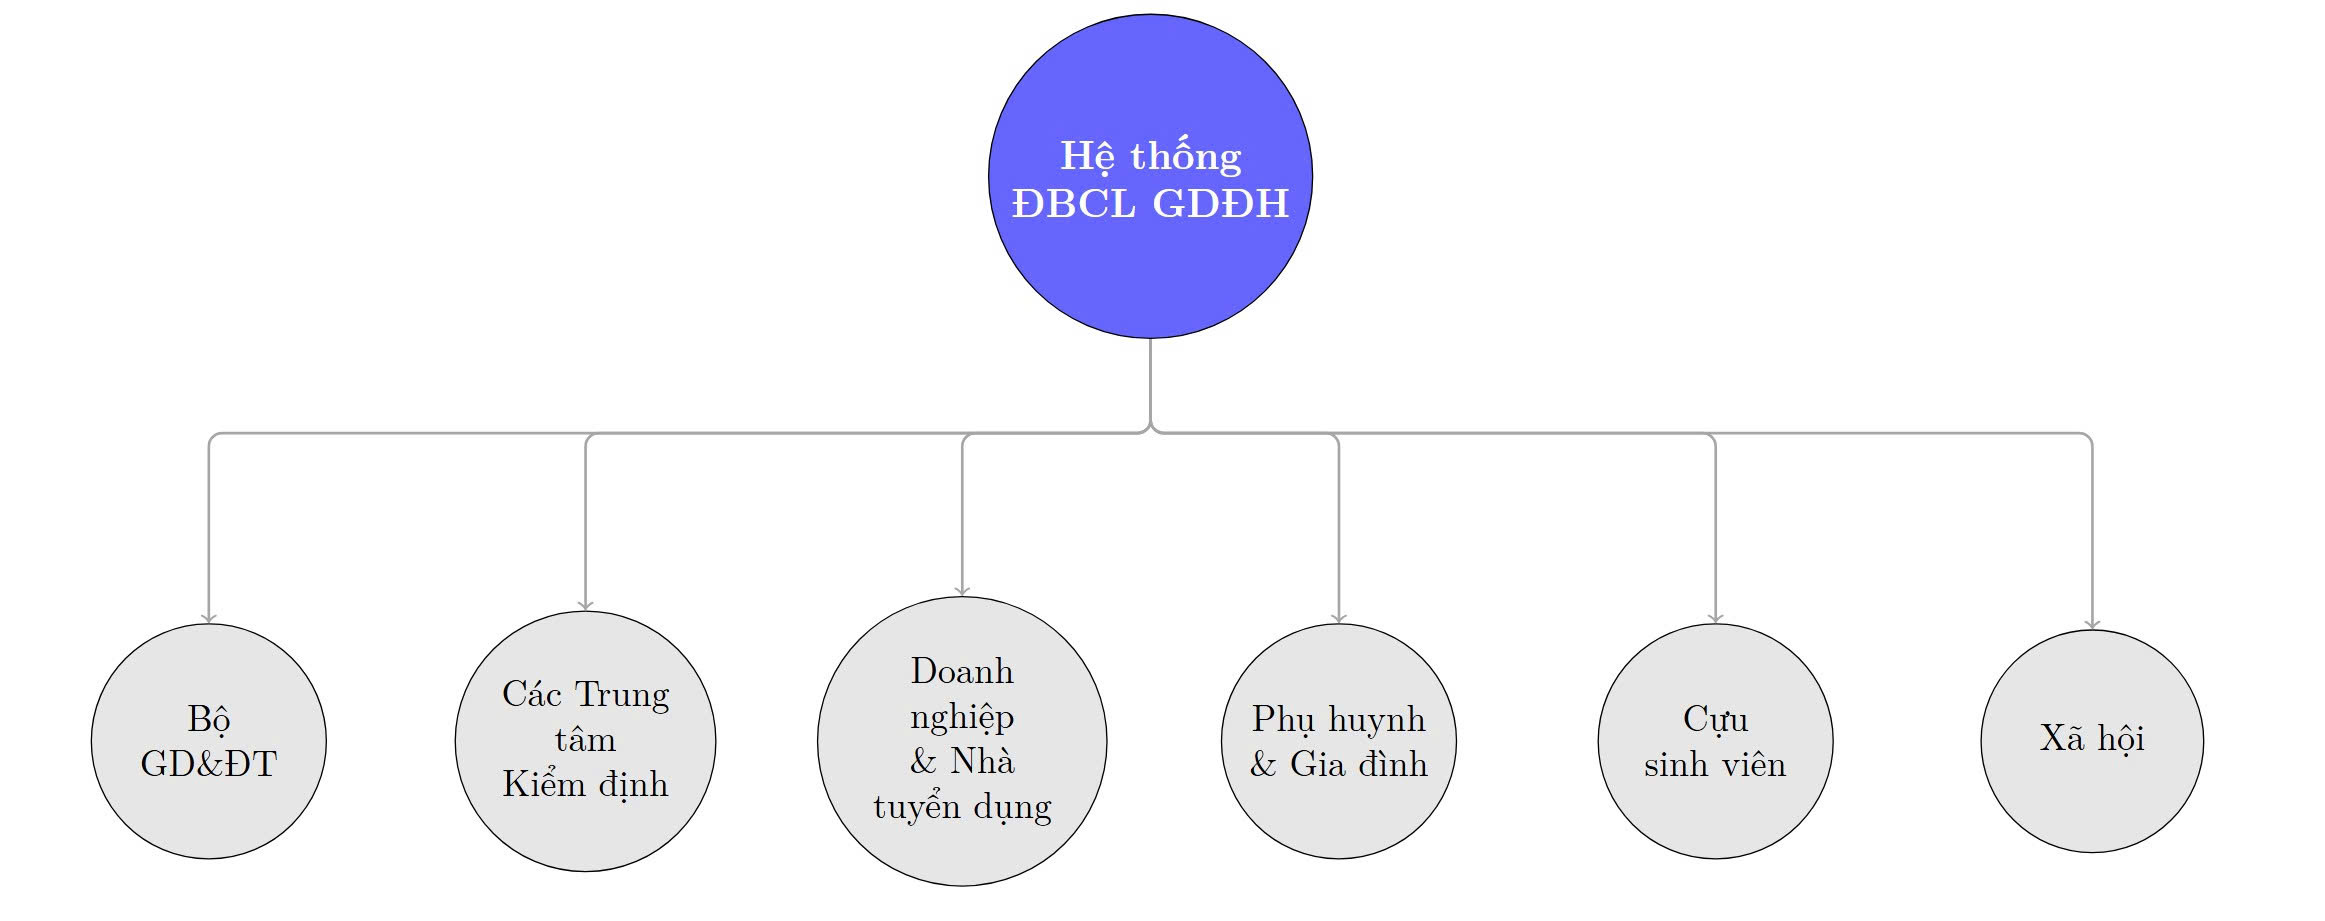
\includegraphics[width=\textwidth]{image/stakeholder_map.jpg} 
    \caption{越南高等教育质量保障体系中的利益相关者地图}
    \label{fig:stakeholder-map}
\end{figure}

\begin{itemize}
    \item \textbf{内部利益相关者 (Internal Stakeholders):}
        \begin{itemize}
            \item \textit{学校领导层(校董会、校领导班子):} 主要利益是学校的声誉、财务稳定、达成KPI指标以及遵守上级规定。
            \item \textit{教师与研究人员:} 利益包括学术自由、良好的工作条件、专业发展机会以及减少行政负担。
            \item \textit{行政人员(包括质量保障处干部):} 利益是流程清晰、有足够资源完成工作以及得到其他部门的合作。
            \item \textit{学生:} 核心利益是培养方案的质量、有效的教学方法、良好的学习环境、毕业后的就业机会以及合理的学费。
        \end{itemize}
    \item \textbf{外部利益相关者 (External Stakeholders):}
        \begin{itemize}
            \item \textit{教育培训部:} 利益是确保高等教育体系稳定运行、质量均衡,满足国家经济社会发展目标,并向政府和社会履行问责。
            \item \textit{教育质量认证中心:} 利益是维持其组织的声誉、专业性和独立性;完成被赋予的认证任务。
            \item \textit{企业与雇主:} 利益是能够招聘到具备与工作要求直接匹配的技能和知识的人力资源,减少再培训成本。
            \item \textit{家长与家庭:} 利益是为子女的投资(时间、金钱)带来应有的回报(孩子有好工作、成才)。
            \item \textit{校友:} 利益是学位证书的价值和母校声誉的提升,从而在职业网络中产生自豪感和机会。
            \item \textit{社会:} 利益是高等教育有助于创造一个公平、进步的社会,提供高质量的人力资源并维护文化价值观。
        \end{itemize}
\end{itemize}
该地图显示,质量保障体系必须服务于一个极其多样化的利益网络。一个质量改进的决策,例如增加学生的实践要求,可能会受到企业的欢迎,但却可能遭到教师(因工作量增加)或财务部门(因成本增加)的反对。识别和分析这些潜在的利益冲突,是构建一个有效的质量保障体系的第一步。



% done chuong 2 goi 2


% ======================================================================
% TRANG 11-13: THUYẾT CÁC BÊN LIÊN QUAN (PHẦN 2)
% ======================================================================

\subsubsection{利益相关者的显著性 (Stakeholder Salience)}

识别利益相关者仅仅是第一步。治理中的一个巨大挑战是如何处理来自这些群体的多样且常常相互矛盾的要求。并非所有利益相关者都具有同等的影响力。Mitchell, Agle和Wood(1997)提出了一个极具影响力的模型,用以确定利益相关者的“显著性”(salience),该模型基于三个核心属性\footcite{Mitchell1997}:

\begin{enumerate}
    \item \textbf{权力 (Power):} 利益相关者将其意志强加于组织之上的能力,迫使组织去做那些若无此压力则不会做的事情。权力可以来自对关键资源(如预算)的控制、颁布法规的能力或影响媒体的能力。
    \item \textbf{合法性 (Legitimacy):} 社会承认某一利益相关者的要求或行动在特定社会背景下是正当、适宜和正确的。合法性来自法律规定、合同或社会道德规范。
    \item \textbf{紧迫性 (Urgency):} 利益相关者的要求需要立即关注的程度。紧迫性取决于两个因素:时间敏感性(若不及时处理,要求将失去价值)和该要求对利益相关者的重要程度。
\end{enumerate}

根据拥有一、二或全部三个属性,利益相关者可被划分为不同优先级的群体,从“潜在”群体(latent stakeholders,仅有1个属性)到需要领导层最多关注的“决定性”群体(definitive stakeholders,拥有全部3个属性)。

将此模型应用于越南高等教育的质量保障体系,我们可以解释一些重要现象:
\begin{itemize}
    \item \textbf{教育培训部}是一个“决定性”利益相关者。该部拥有\textit{权力}(通过分配预算、颁发许可),拥有\textit{合法性}(依据《高等教育法》),并且其要求通常具有\textit{紧迫性}(与认证、报告周期挂钩)。因此,该部的声音分量最重,各大学通常优先满足其要求。
    \item \textbf{企业/雇主}是一个拥有\textit{合法性}(他们有权要求高质量的人力资源)和\textit{紧迫性}(人力需求不断变化)的利益相关者,但却缺乏直接\textit{权力}来迫使大学立即改变培养方案。这解释了为什么尽管企业不断抱怨学生质量,但大学培养方案的变革仍然缓慢。
    \item \textbf{学生和家长}拥有很高的\textit{合法性}和\textit{紧迫性},但他们的权力是分散的。只有当他们的要求通过大规模调查或媒体汇集起来时,他们的权力才会变得更加显著。
\end{itemize}
因此,显著性模型帮助我们理解,质量保障过程并非一个所有声音都平等的绝对民主过程,而是一个“政治舞台”,各大学必须不断权衡并优先考虑来自最具影响力的利益相关者的要求。

\subsubsection{利益相关者理论的应用与批判}

利益相关者理论提供了一个有效的分析工具,用以解读质量保障体系中的利益冲突。它有助于回答“质量为谁服务?”这一问题。通过识别利益相关者并分析其优先级,我们可以理解为什么质量的某些方面(例如:国际论文发表数量)会比其他方面(例如:学生的实践技能)更受重视。

然而,该理论也有其局限性。应用它时最大的挑战在于,当利益相互冲突时,如何找到一个最优方案来\textbf{平衡}这些利益。例如,为满足企业要求而加强实践教学会增加培养成本,可能导致学费上涨,从而引起学生和家长的反对。利益相关者理论很好地描述了这场争论,但并未提供解决它的明确公式。此外,该理论侧重于有形的关系和利益,但较少关注对组织行为有强大影响的无形文化规则和规范——而这正是新制度主义理论的长处。要理解具体的问责机制,我们需要借助第三种理论。

\subsection{委托代理理论 (Principal-Agent Theory)}
\label{subsec:uy_nhiem_nen_tang}

\subsubsection{起源与核心概念}
委托代理理论起源于经济学,特别是金融经济学和公司理论,其基础性工作由Stephen Ross等学者,特别是Michael Jensen和William Meckling在1970年代完成\footcite{JensenMeckling1976}。该理论旨在分析在一方(委托人 - Principal)雇佣或委托另一方(代理人 - Agent)代其执行某项工作时所产生的问题。

这种关系的核心问题(代理问题)源于两个基本条件:
\begin{enumerate}
    \item \textbf{目标冲突 (Conflict of Interest):} 委托人和代理人的利益并非总是一致。例如,股东(委托人)希望最大化利润,而管理者(代理人)可能希望最大化权力或其他个人利益。
    \item \textbf{信息不对称 (Information Asymmetry):} 代理人通常比委托人拥有更多关于工作及自身努力的信息。委托人难以完美地监督代理人的每一个行动。
\end{enumerate}
这两个条件的结合产生了两种主要风险\footcite{Eisenhardt1989}:
\begin{itemize}
    \item \textbf{道德风险 (Moral Hazard):} 合同签订后,由于委托人无法观察其努力程度,代理人可能不会尽全力工作。例如,一所大学(代理人)在从政府(委托人)获得预算后,可能不会尽最大努力投入于改进教学质量。
    \item \textbf{逆向选择 (Adverse Selection):} 签订合同前,代理人可能隐瞒信息或歪曲自身能力以求被选中。例如,一所大学可能会“美化”其自评报告,以获得认证机构的承认。
\end{itemize}
为解决这些问题,该理论提出了设计有效合同、创建激励机制(incentives)以协调利益等解决方案,最重要的是,建立\textbf{监督与报告系统(monitoring and reporting systems)}以减少信息不对称。


% done chuong 2 goi 3


% ======================================================================
% TRANG 16-18: THUYẾT ỦY NHIỆM (PHẦN 2) VÀ PHÊ PHÁN
% ======================================================================

\subsubsection{作为监督和合同机制的质量保障体系}

从委托代理理论的视角来看,整个外部质量保障体系可以被视为一个复杂的监督和合同机制,旨在解决“代理问题”。

\paragraph{多层次的委托代理关系:}
在高等教育中,关系不仅仅是单个委托人与代理人之间的关系。它是一系列相互嵌套的委托代理关系链,使得管理和监督变得复杂\footcite{Borgos2013}。我们可以将越南的这一关系链想象如下:
\begin{itemize}
    \item \textbf{第一层(政府 $\rightarrow$ 教育培训部):} 政府(委托人)将管理和发展国家高等教育体系的任务交给教育培训部(代理人)。
    \item \textbf{第二层(教育培训部 $\rightarrow$ 大学):} 教育培训部(委托人)向各大学(代理人)颁发办学许可并分配预算,期望各大学能够培养出高质量的人力资源并执行服务社会的研究任务。
    \item \textbf{第三层(校领导班子 $\rightarrow$ 院/系):} 校领导班子(委托人)将招生指标和预算分配给各院系(代理人),要求各院系保证其单位的培养和研究质量。
    \item \textbf{第四层(院/系 $\rightarrow$ 教师):} 院长/系主任(委托人)将教学任务分配给每位教师(代理人),并期望他们能以最佳方式完成授课。
\end{itemize}
这一委托代理链的存在解释了为什么来自最高层(政府)的要求在传达到下层时常常会被“干扰”或变形。

\paragraph{质量保障实践中的监督机制:}
为了在上述关系链中最大限度地减少道德风险和逆向选择,质量保障体系发展出了多种具体的监督机制:
\begin{itemize}
    \item \textbf{报告系统 (Reporting Systems):} 自评报告、年度报告、数据统计等要求,正是上级委托人收集下级代理人活动信息的工具。
    \item \textbf{外部认证 (External Accreditation):} 这是一种专门且正式的监督形式。认证机构(如VNU-CEA或AUN-QA)扮演着第三方“审计员”的角色,受委托人(教育培训部)信任,以核实信息并评估各大学(代理人)的活动\footcite{Borgos2013}。这一过程显著减少了信息不对称。
    \item \textbf{基于成果的合同 (Outcome-based Contracts):} 尽管在越南尚不普遍,但世界范围内的趋势是将预算分配与具体的产出结果(例如:学生就业率、国际发表数量)挂钩。这是一种旨在协调委托人与代理人利益的合同形式。
    \item \textbf{声誉建设 (Reputation Building):} 排名系统和公开认证结果也是一种监督机制。一所学校(代理人)的声誉成为一项重要资产,为了保护这项资产,他们有动力按照各委托人(学生、社会)的期望行事。
\end{itemize}

\subsubsection{委托代理理论的应用与批判}

委托代理理论提供了一套锐利的分析工具,用以剖析质量保障体系中的问责结构和监督机制。它逻辑地解释了为何需要报告、检查、定期认证等流程。特别是在分析合同性关系,如国家与被赋予自主权的公立大学之间的关系时,它尤其有用。

然而,机械地将委托代理理论应用于高等教育领域也有其显著的局限性\footcite{RIHE2022}:
\begin{itemize}
    \item \textbf{过分简化目标:} 该理论假设委托人的目标可以被明确定义。但在高等教育中,“质量”是一个多维度且难以衡量的概念。政府的目标可能是发展经济,而社会的目标是公平,学术界的目标则是创作自由。谁才是真正的“委托人”?
    \item \textbf{忽略文化与规范因素:} 该理论认为主体之间的关系主要基于经济利益和理性计算。它无法解释信任、共同价值观以及职业规范(例如:教师道德)在调节教师和学校行为中的作用。
    \item \textbf{难以应用完美的合同:} 在现实中,很难设计一个能预见所有情况并准确衡量代理人所有努力的合同。教育的“产品”(人)是极其复杂的,不能像工业产品那样容易衡量。
\end{itemize}
正因为这些局限性,分析质量保障体系不能仅仅依赖委托代理理论。必须将其与新制度主义理论(以理解无形规则)和利益相关者理论(以理解多样化利益)相结合,才能获得更全面、更准确的图景。

% ======================================================================
% TRANG 19-20: CÁC MÔ HÌNH ĐBCL HIỆN ĐẠI
% ======================================================================
\section{世界现代质量保障模型}
\label{sec:mo_hinh_hien_dai_the_gioi}

治理理论的发展和实践中的挑战,推动了日益精密的质量保障模型的诞生。这些模型不再固守单一理论,而是对传统方法的局限性进行综合和超越的努力。其中,混合模型和适应性框架这两个突出的趋势,对越南具有重要的参考意义\footcite{HybridModel2023}\footcite{AdaptiveQA2022}。

\subsection{混合模型 (Hybrid Model): 协调问责与改进}

\subsubsection{诞生背景与理念}
传统的质量保障体系通常陷入两个极端之一。一是,体系过分注重对外部的\textbf{问责制(accountability)}(自上而下),导致学校只专注于形式上、应付性地遵守规定,形成一种“合规文化”(culture of compliance)而非实质性改进。这是一种接近委托代理理论思维的模式。二是,体系过分注重\textbf{内部改进(improvement)}(自下而上),将全部权力交给单位自行评估,导致缺乏共同标准且难以确保对社会的问责。

混合模型应运而生,旨在解决这种紧张关系\footcite{EUA_Integration}。其理念是承认并整合这两个目标。它认为一个可持续的质量保障体系必须既能满足外部的控制和透明度要求,又能激发内部的改进动力和发展质量文化。混合模型不将问责与改进视为对立的目标,而是视其为一枚硬币的两面,相辅相成。例如,外部透明的问责要求可以为推动内部改进努力提供必要的数据和压力。反之,强大的内部改进文化将使学校更容易满足并超越外部的问责要求。

\subsubsection{组成部分与特点}
一个典型的混合模型通常具有以下特点:
\begin{itemize}
    \item \textbf{双重标准框架:} 体系可能包括一套用于问责目的的强制性\textbf{最低标准(minimum standards)},以及一套用于改进目的的鼓励性\textbf{提升标准(enhancement standards)}。
    \item \textbf{嵌套流程:} 外部认证活动的设计不仅旨在检查合规性,还旨在提供建设性建议,支持学校的改进过程。反之,内部自评和改进活动的结果被用作外部认证轮次中的重要证据。
    \item \textbf{质量保障机构的灵活角色:} 外部质量保障机构不仅扮演“裁判员”的角色,还扮演“伙伴”、“顾问”的角色,在改进过程中为学校提供支持。
\end{itemize}
欧洲质量保障体系的经验,尤其是在博洛尼亚进程之后,显示出向混合模型转变的明显趋势,其中认证流程越来越被设计为服务于质量提升的目标(enhancement-led accreditation)\footcite{EUA_Integration}。越南的实践,既要满足教育培训部的国家标准,又要参与如AUN-QA等区域认证项目,也正显示出一种混合模型正在逐渐形成的迹象,尽管可能尚非完全自觉\footcite{VNU-CEA2023}\footcite{HangNguyen2017}。

% done chuong 2 goi 4



% ======================================================================
% TRANG 21-22: KHUNG THÍCH ỨNG
% ======================================================================

\subsection{适应性框架 (Adaptive Framework): 在变化世界中的质量管理}
\label{subsec:khung_thich_ung}

\subsubsection{与传统方法的比较}
如果说混合模型解决了质量保障\textit{目标}的矛盾,那么适应性框架则解决了在不稳定和复杂环境中\textit{实施流程}的问题。传统的项目管理方法,通常被称为“瀑布模型”(Waterfall Model),遵循一个严格的线性序列:规划 → 设计 → 执行 → 测试 → 交付。该模型假设所有要求和条件都可以从一开始就明确确定,并且在整个过程中环境不会改变。

然而,在高等教育的现实中,尤其是在越南,情况则完全不同。教育部的政策可能改变,劳动力市场的需求波动,教育技术发展迅速,学校的资源也不稳定。采用一个僵化的、长达5年的瀑布式质量保障计划,通常会导致计划在尚未执行完毕时就已经过时。

适应性框架(Adaptive Framework),其源于敏捷软件开发(Agile)领域,正是为了解决这些问题而生\footcite{Wysocki2009}。它不是试图从一开始就制定一个完美的计划,而是将项目分解为短期的、重复的周期。在每个周期结束时,项目团队将重新评估结果,收集反馈,并为下一个周期调整计划。

\subsubsection{适应性框架的核心原则}
一个具有适应性的质量保障框架将基于以下原则运作:
\begin{itemize}
    \item \textbf{迭代学习 (Iterative Learning):} 整个质量保障流程被视为一个学习过程。学校可以不必每5年进行一次大型评估,而是可以针对具体方面(如教学方法、学生服务)进行更小规模的评估周期(例如,每年一次)。每个周期的结果将为改进下一个周期提供信息。
    \item \textbf{反馈循环 (Feedback Loops):} 该框架创建了快速且频繁的反馈循环。学校不必等到5年周期结束才有认证报告,而是可以在每学期或每学年后与学生、教师和企业组织反馈会议。
    \item \textbf{增量发展 (Incremental Development):} 质量改进不必同时进行,而是可以分阶段、逐步实施。例如,第一年,学校可以集中改进学生意见收集系统;第二年,专注于创新学习成果评估方法。
    \item \textbf{价值驱动的优先级排序 (Value-driven Prioritization):} 在每个周期,改进活动将根据其在当时为最重要利益相关者带来的价值来进行优先排序。
\end{itemize}

\subsubsection{对越南国情的适用性}
认为适应性框架特别适合越南国情的论点基于以下原因:
\begin{itemize}
    \item \textbf{动态的政策环境:} 越南关于高等教育的法规和政策可能会迅速变化。一个适应性框架允许学校灵活调整其质量保障策略,以适应新的要求,而无需推翻整个旧计划。
    \item \textbf{资源限制:} 学校不必投入巨额资金进行全面改革,而是可以根据其在每个阶段的有限资源,进行小规模、渐进式的改进。
    \item \textbf{逐步建立能力:} 立即实施一个复杂的质量保障体系可能会给人力团队带来过重负担。适应性框架允许学校边做边学,逐步且可持续地建立质量保障能力。
\end{itemize}
因此,将混合模型的理念与适应性框架的流程相结合,将创造出一种在目标上全面、在实施方式上灵活且务实的质量保障方法。这正是为越南构建建议模型的基础。

% ======================================================================
% TRANG 23-25: ĐỀ XUẤT MÔ HÌNH V-AQA
% ======================================================================
\section{为越南高等教育提出分析模型:混合与适应性模型 (V-AQA)}
\label{sec:mo_hinh_V-AQA_de_xuat}

\subsection{建立一个综合模型的必要性论证}
\label{subsec:luan_giai_V-AQA}
通过以上各部分的分析可以看出,使用单一理论来分析越南高等教育的质量保障体系是不全面的,并可能导致片面的结论。
\begin{itemize}
    \item \textbf{如果仅使用新制度主义},我们将能解释为何各学校会形式化地遵守规定,但难以解释来自内部的实质性改进努力或利益冲突。
    \item \textbf{如果仅使用利益相关者理论},我们将能看到利益多样化的图景,但却缺乏分析工具来解释为何某些方面的声音比其他方面更有分量,也无法解释报告和监督机制。
    \item \textbf{如果仅使用委托代理理论},我们将能清晰理解问责结构,但却会忽略文化、规范因素以及无法简化为单纯合同的复杂合作关系。
\end{itemize}

因此,越南的国情需要一个综合的分析框架,一个能够融合不同视角的模型。本论文提出了这样一个模型,名为\textbf{越南高等教育混合与适应性质量保障模型(The Vietnam - Adaptive Quality Assurance Model,简称 V-AQA)}。

该模型具有\textbf{混合性(Hybrid)},因为它承认并试图协调两个并行且时而矛盾的目标:
\begin{enumerate}
    \item \textbf{对外部的问责制(External Accountability):} 满足教育培训部、认证机构和社会的要求,以获得合法性和资源(反映了新制度主义和委托代理理论的视角)。
    \item \textbf{来自内部的改进(Internal Improvement):} 为内部利益相关者(学生、教师)创造价值,并推动一种内生的质量文化(反映了利益相关者理论的视角)。
\end{enumerate}

同时,该模型具有\textbf{适应性(Adaptive)},因为它在实施过程中强调灵活性,允许大学根据反馈和环境变化,以短期周期调整其质量保障活动,而不是遵循一个僵化的五年计划。

\subsection{V-AQA模型的结构与核心要素}
\label{subsec:cau_truc_V-AQA}

V-AQA模型的结构如同一座神殿,以理论为基石,以最终目标为屋顶,并由五个核心要素作为五根支柱支撑。这五个要素并非独立运作,而是相互作用、相互巩固,形成一个稳固的系统(见图 \ref{fig:v-aqa-model-detailed})。

\begin{figure}[h!]
    \centering
    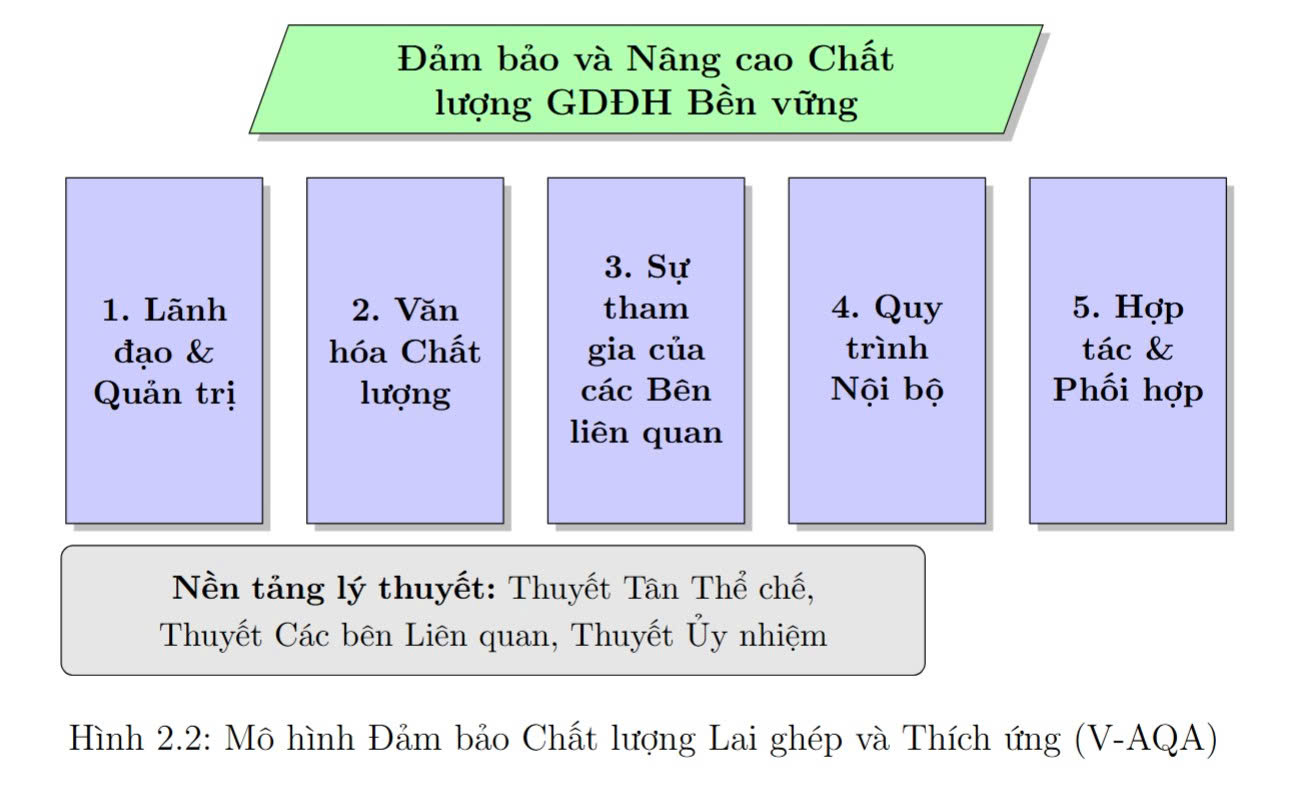
\includegraphics[width=0.9\textwidth]{image/mo_hinh_V-AQA.jpg}
    \caption{混合与适应性质量保障模型 (V-AQA)}
    \label{fig:v-aqa-model-detailed}
\end{figure}

\subsubsection{要素1的详细分析:领导与治理 (Leadership \& Governance)}
\label{subsubsec:thanh_to_1}

\paragraph{定义与范围:}
领导与治理要素是整个质量保障体系的源头,为之指明方向并提供资源。它不仅是行政管理活动,更是领导层在构建愿景、激发灵感以及建立有效治理结构以实现该愿景的能力。在越南的背景下,该要素包括校董会、校领导班子以及各级院、处、室领导的作用。它通过颁布关于质量的战略、政策及执行这些政策的承诺来体现。

\paragraph{理论与实践基础:}
该要素受到\textbf{委托代理理论}和\textbf{新制度主义理论}的强烈映射。
\begin{itemize}
    \item 从委托代理理论的角度看,学校领导层既是上级管理机构(教育培训部)的\textit{代理人},有责任执行国家政策;又是下级单位(院、系)的\textit{委托人},有责任监督并确保这些单位有效运作。明确的治理结构和责任划分是解决内部代理问题的先决条件。
    \item 从新制度主义的角度看,领导者是“解读”并诠释来自制度场域压力的角色。他们决定学校的战略:是被动遵守、模仿成功模式,还是主动寻求独特道路以创造差异化和独特的合法性。领导者的愿景将塑造学校与外部环境互动的方式。
\end{itemize}

\paragraph{实践中的指标与表现:}
为了评估一所大学在该要素上的发展水平,可以考察以下指标:
\begin{itemize}
    \item 是否存在一份详细的校级\textit{质量战略},并将其融入学校的总体发展战略中。
    \item 校领导班子、校董会涉及质量保障问题的会议频率和内容。
    \item 为质量保障活动分配资源(财务、人力)的程度。
    \item 规定质量保障相关单位职能、任务的文件的明确性。
    \item 关于干部、教师对领导层在质量工作中的承诺和导向作用的意见调查结果。
\end{itemize}
对这些指标的分析将在本论文的现状章节中详细进行。

% done chuong 2 goi 5


% ======================================================================
% TRANG 26-28: PHÂN TÍCH CHI TIẾT THÀNH TỐ 2: VĂN HÓA CHẤT LƯỢNG
% ======================================================================

\subsubsection{要素2的详细分析:质量文化 (Quality Culture)}
\label{subsubsec:thanh_to_2}

\paragraph{定义与范围:}
质量文化不仅是对质量的认知或口号,而是一个共享的价值观、信念、期望和承诺的集合,它塑造了一个教育机构中所有成员在保障和提升质量方面的行为\footcite{HarveyStensaker}。它是在谈论质量时“我们在这里做事的方式”(the way we do things around here)。该要素与“合规文化”(culture of compliance)相对立,在合规文化中,质量保障活动只是为了应付外部要求而机械地执行。

质量文化的范围非常广泛,它渗透到学术生活的每一个角落,从一名教师如何准备教案,一个院系如何组织专业研讨会,到学校领导层如何做出战略决策。一个强大的质量文化将把质量保障从一种行政负担转变为个人和组织发展的内在动力。

\paragraph{理论基础与质量文化的维度:}
质量文化通过\textbf{新制度主义理论}的视角得到最清晰的体现,特别是其\textit{规范性(normative)}和\textit{文化-认知性(cultural-cognitive)}两大支柱。
\begin{itemize}
    \item \textbf{规范性方面:} 质量文化通过职业规范形成和巩固。当“持续改进”或“以学习者为中心”成为学术界所重视的规范时,个人为了被视为专业的教育者和管理者,会倾向于按照该规范行事。
    \item \textbf{文化-认知性方面:} 质量文化作为一种无需思考即被接受的脚本或常识而存在。届时,收集学生反馈或定期审查培养方案不再是一项要求,而是一件“理所当然”必须做的事情。
\end{itemize}

为了系统地分析质量文化,可以使用Harvey和Stensaker(2008)的模型,该模型将质量文化分为四种类型,反映了组织的成熟度\footcite{HarveyStensaker}:
\begin{enumerate}
    \item \textbf{反应型文化 (Reactive Culture):} 组织仅在出现问题或有外部检查要求时才关注质量。这是最低的层次。
    \item \textbf{响应型文化 (Responsive Culture):} 组织开始建立流程和体系以响应质量要求,但动力主要仍来自外部。许多越南大学目前正处于此阶段,为应对认证评估而建立质量保障部门和流程。
    \item \textbf{再生/改进型文化 (Regenerative Culture):} 这是一个质的飞跃。组织有能力自我评估,自我发现问题,并主动实施持续改进的循环。改进的动力来自内部。
    \item \textbf{繁殖/传播型文化 (Reproductive Culture):} 在最高层次,组织不仅自我改进,还成为典范,向外传播关于质量的最佳实践,为其他组织塑造规范。
\end{enumerate}
该模型为诊断和确定一所大学质量文化的发展目标提供了有用的工具。

\paragraph{在越南实践中的指标与表现:}
质量文化是一个抽象的概念,但可以通过具体的指标和表现来间接衡量:
\begin{itemize}
    \item \textbf{领导层的承诺:} 公开发言、战略文件以及资源分配是否显示出质量保障是真正的优先事项。
    \item \textbf{教师和员工的态度:} 关于工作满意度、对质量保障活动(视其为负担还是机遇)的态度的调查结果,以及自愿参与改进活动的程度。
    \item \textbf{内部使用的语言:} 内部文件和会议是使用“遵守”、“响应要求”的语言,还是“提升”、“改进”、“卓越”的语言?
    \item \textbf{认可与奖励机制:} 学校是否有机制来表彰和奖励有质量改进创举的个人和单位?
\end{itemize}
正如专家报告所反映的,越南的现状表明,许多大学仍在努力从“响应型”文化向“改进型”文化转型。来自认证评估的压力通常会产生临时性的活动,质量文化尚未真正深入到每位教师的日常工作中\footcite{ExpertPerspectivesVN}\footcite{CommonFailureCriteria}。这是V-AQA模型需要解决的最大挑战之一。

% ======================================================================
% TRANG 29-30: PHÂN TÍCH CHI TIẾT THÀNH TỐ 3: SỰ THAM GIA CỦA CÁC BÊN LIÊN QUAN
% ======================================================================

\subsubsection{要素3的详细分析:利益相关者的参与 (Stakeholder Engagement)}
\label{subsubsec:thanh_to_3}

\paragraph{定义与范围:}
利益相关者的参与不仅仅是“征求意见”或“举办研讨会”。它是一个有系统的、有目的的过程,旨在将利益相关者吸引到质量保障的各个环节中,从培养方案的设计,到教与学的过程,再到评估和改进。这是“质量为谁服务?”这一理念的实现,承认一个高质量的培养方案必须为不同的对象群体创造价值。

参与的范围很广,包括从低到高的多种形式:
\begin{itemize}
    \item \textbf{告知 (Informing):} 向利益相关者单向提供信息。
    \item \textbf{咨询 (Consulting):} 征求利益相关者的意见和反馈。
    \item \textbf{卷入 (Involving):} 在整个过程中与利益相关者直接合作。
    \item \textbf{协作 (Collaborating):} 在决策中成为合作伙伴。
    \item \textbf{授权 (Empowering):} 将最终决策权交给利益相关者。
\end{itemize}
一个成熟的质量保障体系需要根据具体问题和具体利益相关者,为不同层次的参与提供机制\footcite{Arnstein1969}。

\paragraph{理论与实践基础:}
该要素是\textbf{利益相关者理论}的直接应用。它将重心从一个封闭、内向的管理模式转向一个开放、外向的模式。这也是混合模型的一个核心要素,因为正是来自外部利益相关者的反馈和要求,构成了内部改进活动的重要动力。

国际实践,特别是欧洲的经验表明,利益相关者,尤其是学生和雇主的参与,是现代质量保障体系中不可或`缺的要素。像AUN-QA这样的标准体系也对在审查和改进培养方案中收集和使用利益相关者反馈提出了明确要求\footcite{ENQA_Stakeholder2018}\footcite{AUN-QAGuide}。

\paragraph{在越南实践中的指标与表现:}
该要素的发展水平可以通过以下指标进行评估:
\begin{itemize}
    \item \textbf{有外部人员参与的委员会的存在:} 例如,科学与培养委员会、每个专业的行业咨询委员会(Industry Advisory Board)。
    \item \textbf{咨询活动的频率和实质性:} 与雇主举行的研讨会数量、校友调查、为学生设立的反馈渠道。
    \item \textbf{影响的证据:} 是否有具体证据表明培养方案已根据企业或校友的反馈进行了调整和更新。
    \item \textbf{学生在各委员会中的角色:} 学生在院级、校级委员会中是否有代表,他们的声音是否得到实质性的倾听和记录。
\end{itemize}
在越南,这是仍存在诸多局限的要素之一。报告通常指出,校企联系仍然松散且形式化。培养方案的制定通常主要基于学术团队的观点,而很少有雇主的实质性参与\footcite{CommonFailureCriteria}。因此,加强利益相关者的参与是越南高等教育质量保障体系改革的一个重要方向。

% done chuong 2 goi 6


% ======================================================================
% TRANG 31-35: PHÂN TÍCH CHI TIẾT THÀNH TỐ 4: QUY TRÌNH NỘI BỘ
% ======================================================================

\subsubsection{要素4的详细分析:内部流程 (Internal Processes)}
\label{subsubsec:thanh_to_4}

\paragraph{定义与范围:}
如果说前面的要素关注的是“为什么”(理论)、“谁”(领导者、利益相关者)和“什么”(文化),那么要素4则关注\textbf{“如何做?”}的问题。内部流程是一所教育机构用来系统地管理核心学术活动以保障和提升质量的一整套标准化的政策、程序、指南和工具。

这是质量保障体系的“运行机器”,将质量战略和目标转化为具体且可衡量的行动。该要素的范围涵盖了学生的整个学术生命周期,从培养方案的设计到学生毕业并由雇主评估。在本论文的框架内,我们将重点关注三个最重要的子流程:(1)培养方案(CDĐT)的设计与审查;(2)教-学活动与评估的管理;以及(3)数据收集与分析系统。

\paragraph{子流程4.1:培养方案(CDĐT)的设计与审查}
这是决定学校所提供的教育“产品”的基础流程。一个有效的流程必须确保培养方案既具科学性,又能满足利益相关者的需求。

\textit{理论基础:} 该流程是三大基础理论的交汇点。\textbf{利益相关者理论}要求流程必须有机制来收集和整合来自学生、企业的要求。\textbf{新制度主义理论}解释了为什么培养方案通常必须遵守教育培训部颁布的“课程框架”(强制性同形),并倾向于参考知名大学(模仿性同形)。\textbf{委托代理理论}将培养方案视为学校(代理人)承诺为社会和国家(委托人)执行的一种详细“合同”。

\textit{标准流程中的步骤:} 一个有效的培养方案设计与审查流程通常包括以下步骤,正如AUN-QA等国际标准所建议的\footcite{AUN-QAGuide}:
\begin{enumerate}
    \item \textbf{确定预期学习成果(Expected Learning Outcomes - ELOs):} 这是最重要的一步。ELOs必须基于与利益相关者(特别是雇主)的协商来制定,必须清晰、可衡量,并与学校的使命和愿景相符。
    \item \textbf{构建课程地图(Curriculum Mapping):} 设计课程和学习活动,使其能够逻辑地、系统地为实现既定的ELOs做出贡献。该技术有助于确保整个方案的一致性和建设性对齐(constructive alignment)。
    \item \textbf{审批与颁布:} 必须有一个科学与培养委员会(有外部专家参与)在正式颁布前对培养方案进行审定和批准。
    \item \textbf{定期审查与改进:} 必须有一个定期流程(例如:每2-3年一次),根据来自校友、雇主的反馈、学生的学习成果以及行业的新趋势来重新审查培养方案。
\end{enumerate}

\textit{越南现状:} 这是仍然存在许多薄弱环节的领域之一。认证报告通常指出,许多学校的培养方案设计流程仍然是封闭的,主要依赖于教师团队的经验,而缺乏企业的实质性参与。课程审查通常没有系统地进行,导致培养方案落后于劳动力市场的要求\footcite{CommonFailureCriteria}。

\paragraph{子流程4.2:教-学活动与评估的管理}
如果说培养方案是“设计图”,那么这就是“施工”过程。教-学活动和评估的质量直接决定了学生的学习体验和学习成果。

\textit{理论基础:} \textbf{委托代理理论}解释了监督教学活动(听课、检查)的必要性,以减少道德风险(教师备课不认真)。\textbf{利益相关者理论}强调了学生通过调查系统对教学质量提供反馈的作用。

\textit{流程的组成部分:}
\begin{itemize}
    \item \textbf{教学管理流程:} 包括关于制定详细课程大纲、准备教案、应用积极教学方法以及听课、向教师提建议的机制的规定。
    \item \textbf{学生学习成果评估流程:} 需要多样化评估形式,不仅仅依赖期末考试。过程性评估、项目、演讲、团队合作以及基于实践能力的测试等形式需要被标准化并广泛应用。必须有建立试题库、出题、阅卷和复核的透明、公平的流程。
    \item \textbf{反馈流程(Feedback):} 必须有机制让学生定期对每门课程和教师提出反馈。更重要的是,必须有流程来处理这些反馈,并向学生通报已进行的改变和改进。
\end{itemize}

\textit{越南现状:} 这也是一个固有的弱点。认证报告经常指出,单向讲授法被滥用,评估方法主要依赖记忆,以及来自学生的反馈系统仍然是形式化的,并未真正影响到教学的改进\footcite{ExpertPerspectivesVN}\footcite{CommonFailureCriteria}。

\paragraph{子流程4.3:数据收集与分析系统 – 基于证据的治理基础}

这是整个质量保障体系的“神经系统”,是支持其他流程的最重要的技术要素。没有它,所有改进决策都有可能变得主观和缺乏依据。

\textit{理论基础与作用:} 该系统是\textbf{委托代理理论}中监督机制的实现,是倾听\textbf{利益相关者}声音的工具,也是\textbf{新制度主义理论}下专业化、合理化的一个象征。它使学校能够从基于经验的管理模式转向基于证据的治理(evidence-based governance)。

\textit{核心功能:}
\begin{enumerate}
    \item \textbf{收集 (Collection):} 建立流程,从多个来源(学生学习成果、招生数据、教师人事信息、满意度调查结果、校友就业数据、财务数据等)一致地、定期地收集数据。
    \item \textbf{管理 (Management):} 构建一个集中的数据库(database)或数据仓库(data warehouse)来存储、清理和管理已收集的数据。
    \item \textbf{分析 (Analysis):} 使用统计和分析工具将原始数据转化为有意义的信息。例如:寻找教学方法与学生学习成果之间的相关性,或分析影响学生辍学率的因素。
    \item \textbf{报告与可视化 (Reporting \& Visualization):} 构建自动化的报告(reports)和仪表盘(dashboards)系统,直观地为不同级别的管理层提供信息,以支持决策。
\end{enumerate}

\textit{越南现状:} 这被认为是越南质量评估报告中最大和最普遍的挑战\footcite{CommonFailureCriteria}\footcite{AUN-QA_Challenges_VN}。学校通常缺乏一个集成的数据系统;数据分散在不同的部门,没有标准化,难以利用。决策通常仍然更多地依赖于领导的经验,而不是客观的数据分析。构建这样一个系统需要对技术和人力进行大量投资,这是一个巨大的障碍。

\paragraph{关于内部流程要素的结论:}
这三个子流程相互之间联系紧密。一个设计良好的培养方案(4.1)如果不能通过有效的教-学和评估方法(4.2)来实施,将毫无意义。而要知道流程(4.1)和(4.2)是否有效,学校需要一个强大的数据系统来衡量和分析(4.3)。任何一个流程的薄弱都会影响到整个系统。因此,标准化和改进这些内部流程是任何质量保障努力的核心任务。

% done chuong 2 goi 7




















	
%======================================================================
% GÓI 1 (VIẾT LẠI): MỞ ĐẦU VÀ BẰNG CHỨNG VĨ MÔ VỀ "NGHỊCH LÝ PHÁT TRIỂN"
% (Phần 1: Tăng trưởng và Thành tựu)
%======================================================================

\chapter{越南外部质量保障体系现状分析}
\label{chap:thuc_trang}

\section*{引言}
\addcontentsline{toc}{section}{引言}

本章将对越南高等教育(GDĐH)外部质量保障(ĐBCL)体系的现状进行深入和多维度的分析,重点关注2015年至2024年这一强劲转型阶段。本章将运用第二章所论证的V-AQA理论模型视角,重点“解剖”一个深刻的\textbf{发展悖论(development paradox)}:即规模和投入指标的爆炸性增长,并未伴随着产出质量及与劳动力市场契合度的相应提升。

通过综合分析宏观统计数据、世界银行等权威国际组织的报告、学术研究,特别是通过图表进行可视化的数据,本章将提供坚实的科学论据。目标不仅是描述现状,更是要解释阻碍质量提升努力的系统性“瓶颈”和“恶性循环”。从而,本章将为后续章节提出战略性解决方案奠定坚实的实践基础。

\section{越南高等教育中的发展悖论}
\label{sec:nghich_ly_phat_trien_vimo}

2015-2024年阶段标志着越南高等教育一个充满变动的转型历程,揭示了一个深刻的发展悖论。一方面,该体系在教育大众化、扩大培养规模以及提升投入资源质量方面取得了前所未有的成就。另一方面,这些关于“量”的成就,却掩盖了关于“质”的持续挑战,体现在毕业生技能与劳动力市场实际需求之间日益扩大的不匹配。分析此悖论的两个方面,是理解该体系核心挑战的先决条件。

\subsection{悖论的第一面:规模的爆炸性增长与投入资源的改善}
\label{subsec:ve_thu_nhat_nghich_ly}

不可否认,越南高等教育在扩大民众教育机会方面取得了令人瞩目的进展。这一时期见证了强劲的大众化进程,体现在办学机构网络的拓展和学生规模的飞跃式增长。

\subsubsection{拓展教育网络与培养规模}

过去十年越南高等教育体系发展的全貌,通过图\ref{fig:so_truong_quy_mo_sv}得以清晰展现。

\begin{figure}[h!]
    \centering
    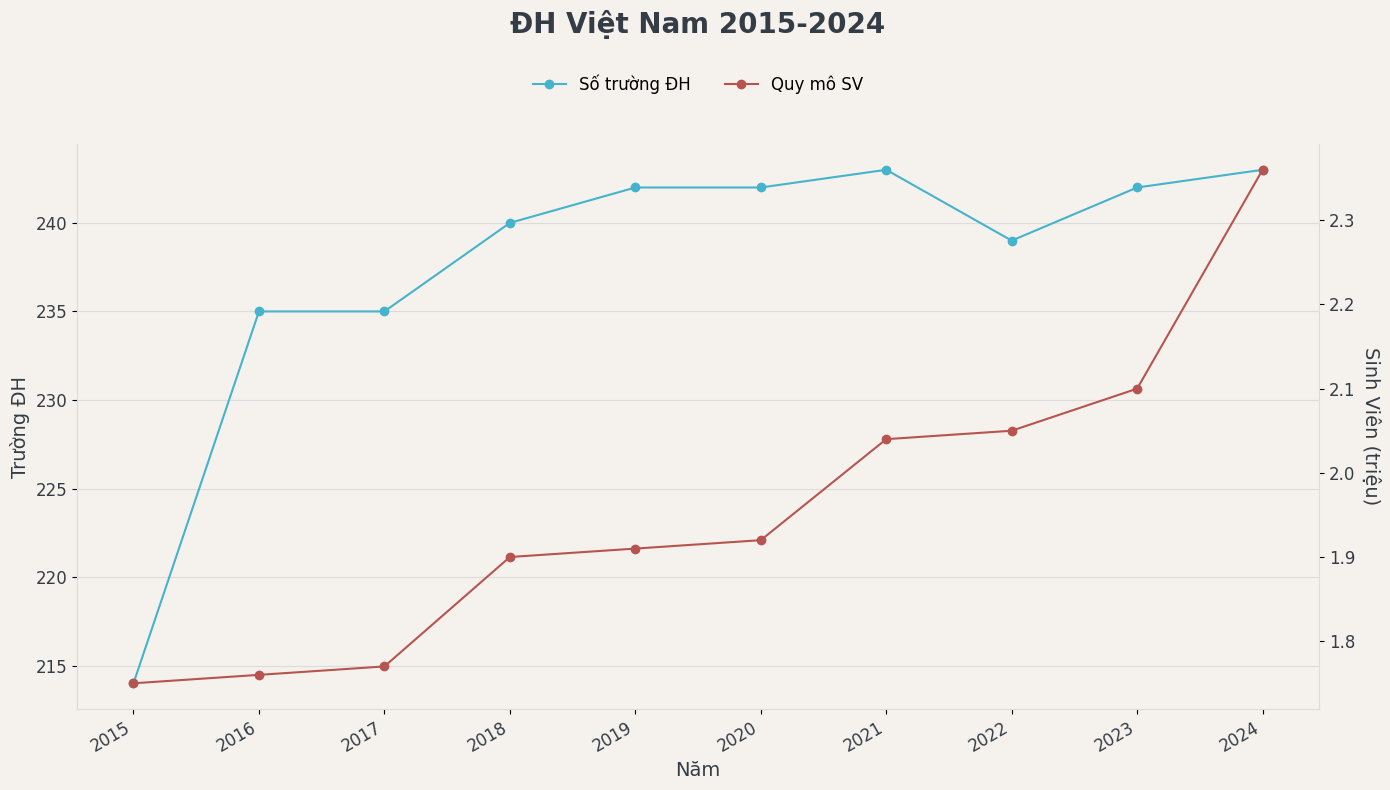
\includegraphics[width=\textwidth]{image/dh_viet_nam_2015_2024.png}
    \caption{越南高等教育办学机构数量与学生规模发展情况(2015-2024年)}
    \label{fig:so_truong_quy_mo_sv}
\end{figure}

分析图\ref{fig:so_truong_quy_mo_sv}显示了两种同步但速度不同的增长趋势。
\begin{itemize}
    \item \textbf{关于网络(蓝色线):} 高等教育机构数量呈现稳定而坚实的增长趋势,从2015年的215所增至2024年的243所。这一增长虽然不算突变,但反映了政府在拓展办学机构网络方面的一贯政策,包括成立新大学和升级专科学校,旨在为全国民众提供多样化的学习机会。
    \item \textbf{关于学生规模(红色线):} 与学校数量的平稳增长形成对比的是,学生规模呈现出异常强劲的爆炸性增长。在经历了2015年至2021年的相对稳定期后,学生规模在最后三年(2022-2024)内从约205万猛增至超过\textbf{235万学生}。这一飞跃不仅体现了高等教育日益增长的吸引力,也表明该体系正承受着为前所未有的大量学生提供培养需求的巨大压力。
\end{itemize}

这一增长正逐步使越南更接近到2030年实现\textbf{每万人口260名大学生}的国家战略目标\footcite{sggp_en_3million_2030}。此外,它还体现在重要的国际指标——高等教育毛入学率(GER)上。世界银行和联合国教科文组织的数据显示,越南的毛入学率已从2000年的仅10.3\%飙升至2018年的28.6\%,并于\textbf{2022年达到创纪录的42.22\%}\footcite{worldbank_humancapital_2022}。这是一项值得称道的成就,显示了教育大众化政策的成功。

\subsubsection{改善投入资源质量}
在扩大规模的同时,该体系的投入资源质量也取得了显著改善,显示了在提升内在能力方面的有目的的投资。
\begin{itemize}
    \item \textbf{师资队伍质量:} 拥有研究生学历(硕士或博士)的大学教师比例几乎翻了一番,从2007年的47\%增至\textbf{2020年达到85\%}\footcite{worldbank_p178112}。对提升师资队伍水平的投资是一个基础性因素,有望直接转化为教学和研究质量。
    \item \textbf{科学研究能力:} 提升教师水平的成就已产生具体影响。越南人均在国际权威期刊上可引用的科学文献数量,在十年间(2010-2020)\textbf{增长了三倍}\footcite{worldbank_improvingperformance_2020}。这表明该体系的研究能力取得了飞跃式进展,正逐步与国际科学界接轨。
\end{itemize}

上述数字和图表描绘了一幅关于悖论第一面的乐观画面:一个正在强劲发展、在网络、学生规模乃至投入资源质量等各方面都在扩张的高等教育体系。这些是不可否认的成就,为一个现代化和国际化的高等教育体系奠定了坚实的基础。然而,这幅画面只是一个更为复杂的悖论的一半。当我们将这些关于“量”的成就与关于产出质量和体系效率的指标进行对比时,一个充满挑战和警示的另一面故事开始显现。悖论的第二面将在下一部分深入分析。



% het goi 1


\subsection{悖论的第二面:质量的潜在危机与不匹配}
\label{subsec:ve_thu_hai_nghich_ly}

与规模和投入资源令人印象深刻的增长图景相反的是,关于产出质量和体系可持续性的 alarming signals。如果说悖论的第一面是一曲增长数字的交响乐,那么第二面则是一个残酷的现实,体现在培养规模与满足劳动力市场能力之间的分化。图\ref{fig:nghich_ly_quy_mo_chat_luong}清晰地将这一悖论可视化。

\begin{figure}[h!]
    \centering
    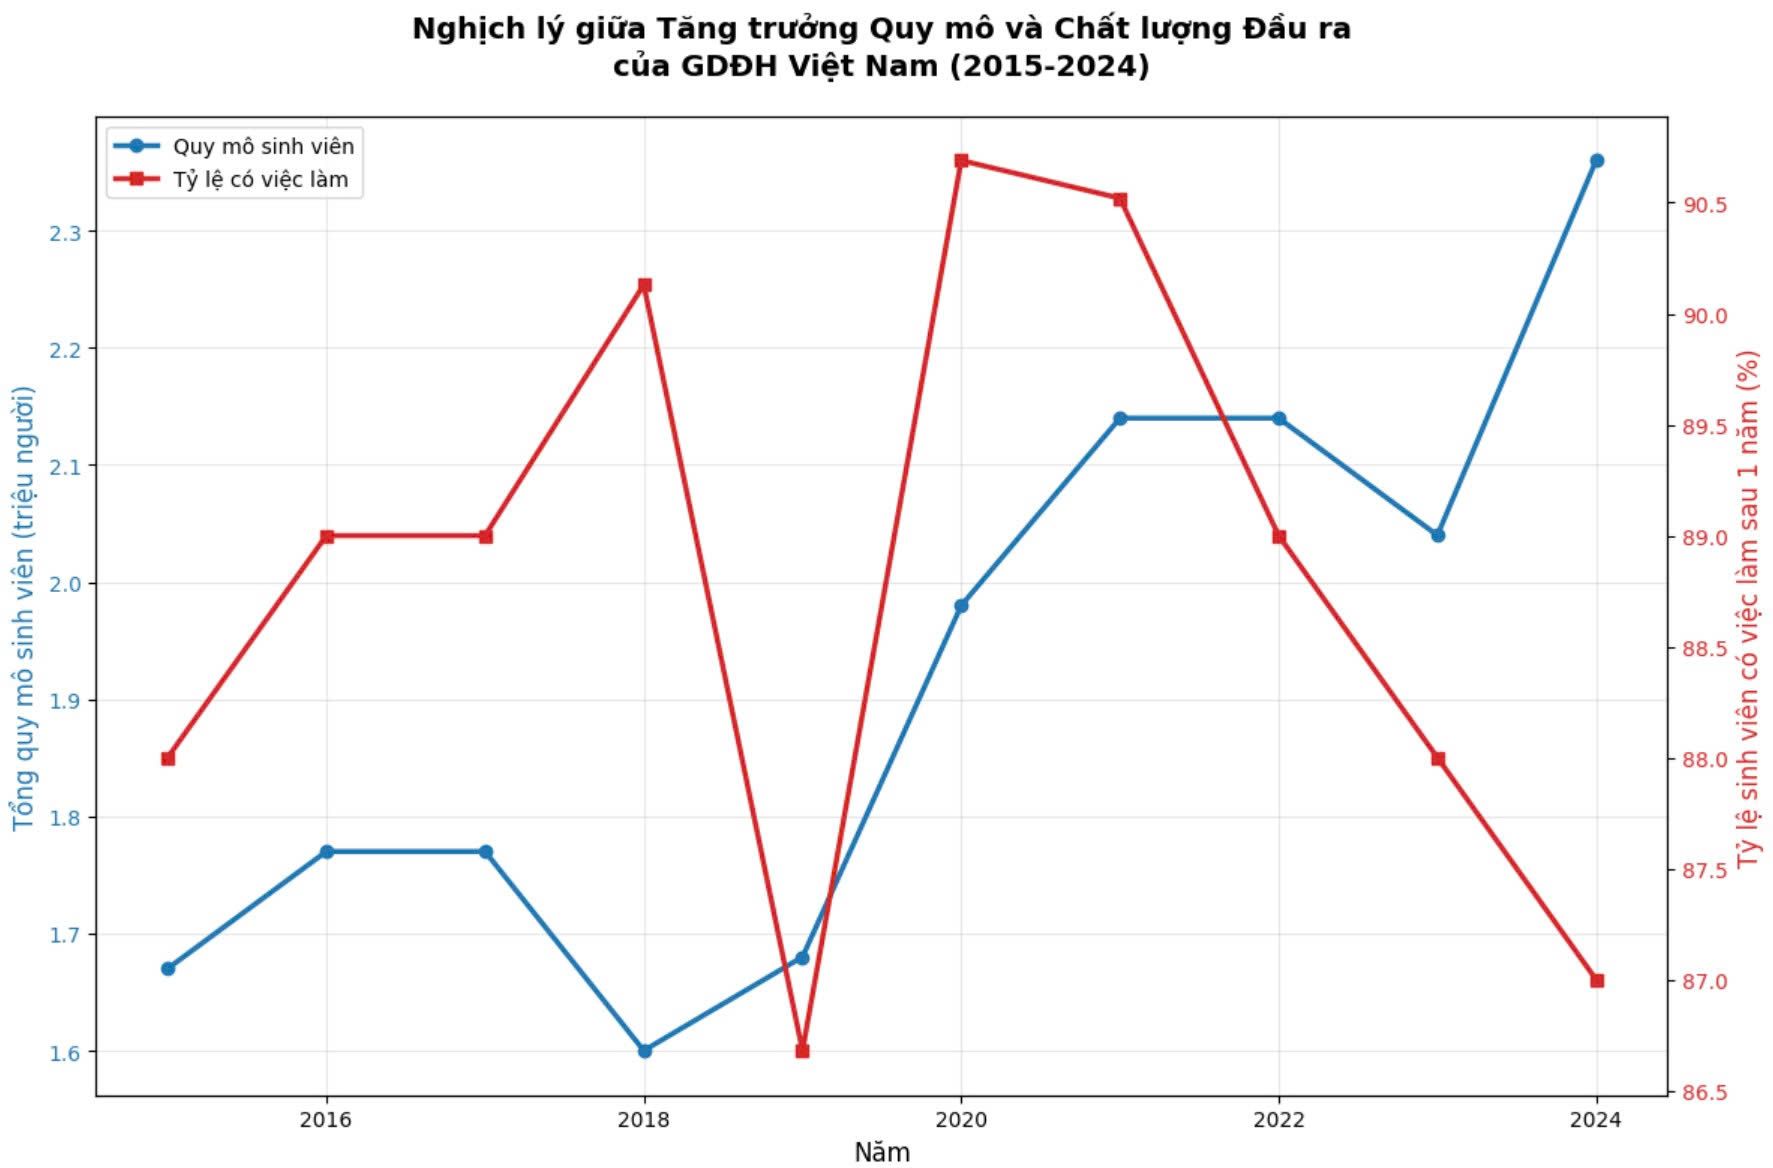
\includegraphics[width=\textwidth]{image/nghich_ly_tang_truong_quy_mo_chat_luong.jpg}
    \caption{越南高等教育规模增长与产出质量之间的悖论(2015-2024年)}
    \label{fig:nghich_ly_quy_mo_chat_luong}
    \vspace{0.2cm}
    \footnotesize{\textit{来源:综合整理自教育培训部数据及相关报告。}}
\end{figure}

\subsubsection{剖析“量”与“质”的分化}

图\ref{fig:nghich_ly_quy_mo_chat_luong}将两个重要指标置于同一坐标系中:学生总规模(左纵轴,蓝色线)和毕业一年后就业率(右纵轴,红色线)。理论上,在一个可持续发展的体系中,这两条线应呈正相关或至少保持稳定。然而,实际数据显示出一种令人担忧的分化(divergence):
\begin{itemize}
    \item \textbf{规模线(蓝色)}呈现出持续增长,特别是从2020年不到200万学生猛增至2024年超过230万学生。这再次证实了该体系面临的扩大规模的压力。
    \item \textbf{质量线(红色)}则呈现出完全相反的趋势。在2019-2020年左右达到峰值(超过90%)后,学生就业率出现了惊人的急剧下降,到2024年降至仅约87%。
\end{itemize}
这种分化正是发展悖论的“核心”:当体系在规模上日益“膨胀”时,其最核心的价值——帮助学习者获得就业并为社会做贡献的能力——却在下降。这提出了一个紧迫的问题:难道对数量的追求已经严重损害了质量?

\subsubsection{来自劳动力市场的证据:失业、技能差距与不平等}

图表中“质量”线的下降趋势并非感性判断,而是由一系列来自劳动力市场和社會學分析的確鑿數據所證實。

\paragraph{失业与学非所用。} 劳动荣军与社会部的报告多次警示本科毕业生失业率高企,\textbf{2017年高达23.7万人},2018年仍有\textbf{22.55万人},约占全国失业总人数的20\%\footcite{vietnamnews_unemployed_2017}。这一数字,加上估计约有\textbf{60\%的毕业生从事与专业不符的工作},是因培养与需求脱节而造成社会和个人资源浪费的明显证据\footcite{britishcouncil_grad_employability_2021}。

\paragraph{技能差距。} 上述状况的深层原因在于严重的“技能差距”。英国文化协会的一项全面调查指出了一个令人担忧的现实:\textbf{73\%}的越南企业在招聘具备领导和管理技能的人才时遇到困难;\textbf{68\%}在寻找具备足够专业技能的员工时遇到困难;\textbf{54\%}表示缺乏具备必要社交情感技能的人才\footcite{britishcouncil_skills_gap_2021}。世界银行的报告也强调,近\textbf{80\%}的制造业公司在招聘熟练工人时遇到困难\footcite{worldbank_p178112}。这表明培养方案并未能为学生充分装备经济真正需要的技能。

\paragraph{机会不均与财务负担。} 除了质量问题,发展悖论还体现在不平等方面。尽管越南高等教育的个人回报率位居世界最高之列(年均超过15\%)\footcite{worldbank_improvingperformance_2020},但这一利益并未得到公平分配。数据显示,高达\textbf{80\%来自收入最高20\%家庭的青年}已经或正在接受大学教育,而这一比例在两个最低收入组中仅占学生总数的10\%\footcite{worldbank_p178112}。由于成本负担日益转向家庭(占公立学校总收入的\textbf{77\%})以及学生贷款项目的缩减,这种不平等正面临着加剧的风险\footcite{worldbank_p178112}。

总之,悖论的第二面展示了一幅充满挑战的图景:一个尽管在规模和资源上投入巨大,但其产出却未能满足市场要求,同时潜藏着社会不平等风险的体系。清晰地认识这一悖论的两个方面,是能够准确“诊断”系统性“病症”的先决步骤,这一任务将在本章的后续部分进行。


% het goi 2



\section{塑造质量的主体与制度框架}
\label{sec:khung_the_che}

从已证明的“发展悖论”图景中,一个核心问题被提出:体系中的哪些力量和主体,以何种方式行动,从而造成了这一现状?要回答这个问题,首先需要识别主要的利益相关者,并分析主导该体系“游戏规则”的制度框架。

\subsection{高等教育质量保障生态系统中的利益相关者图}

越南高等教育质量保障体系是一个复杂的生态系统,有众多利益相关者参与其中,每一方都扮演着不同的角色、拥有不同的利益和影响力。图\ref{fig:so_do_he_thong_dbcl}提供了该生态系统中主要主体的概览。

\begin{figure}[h!]
    \centering
    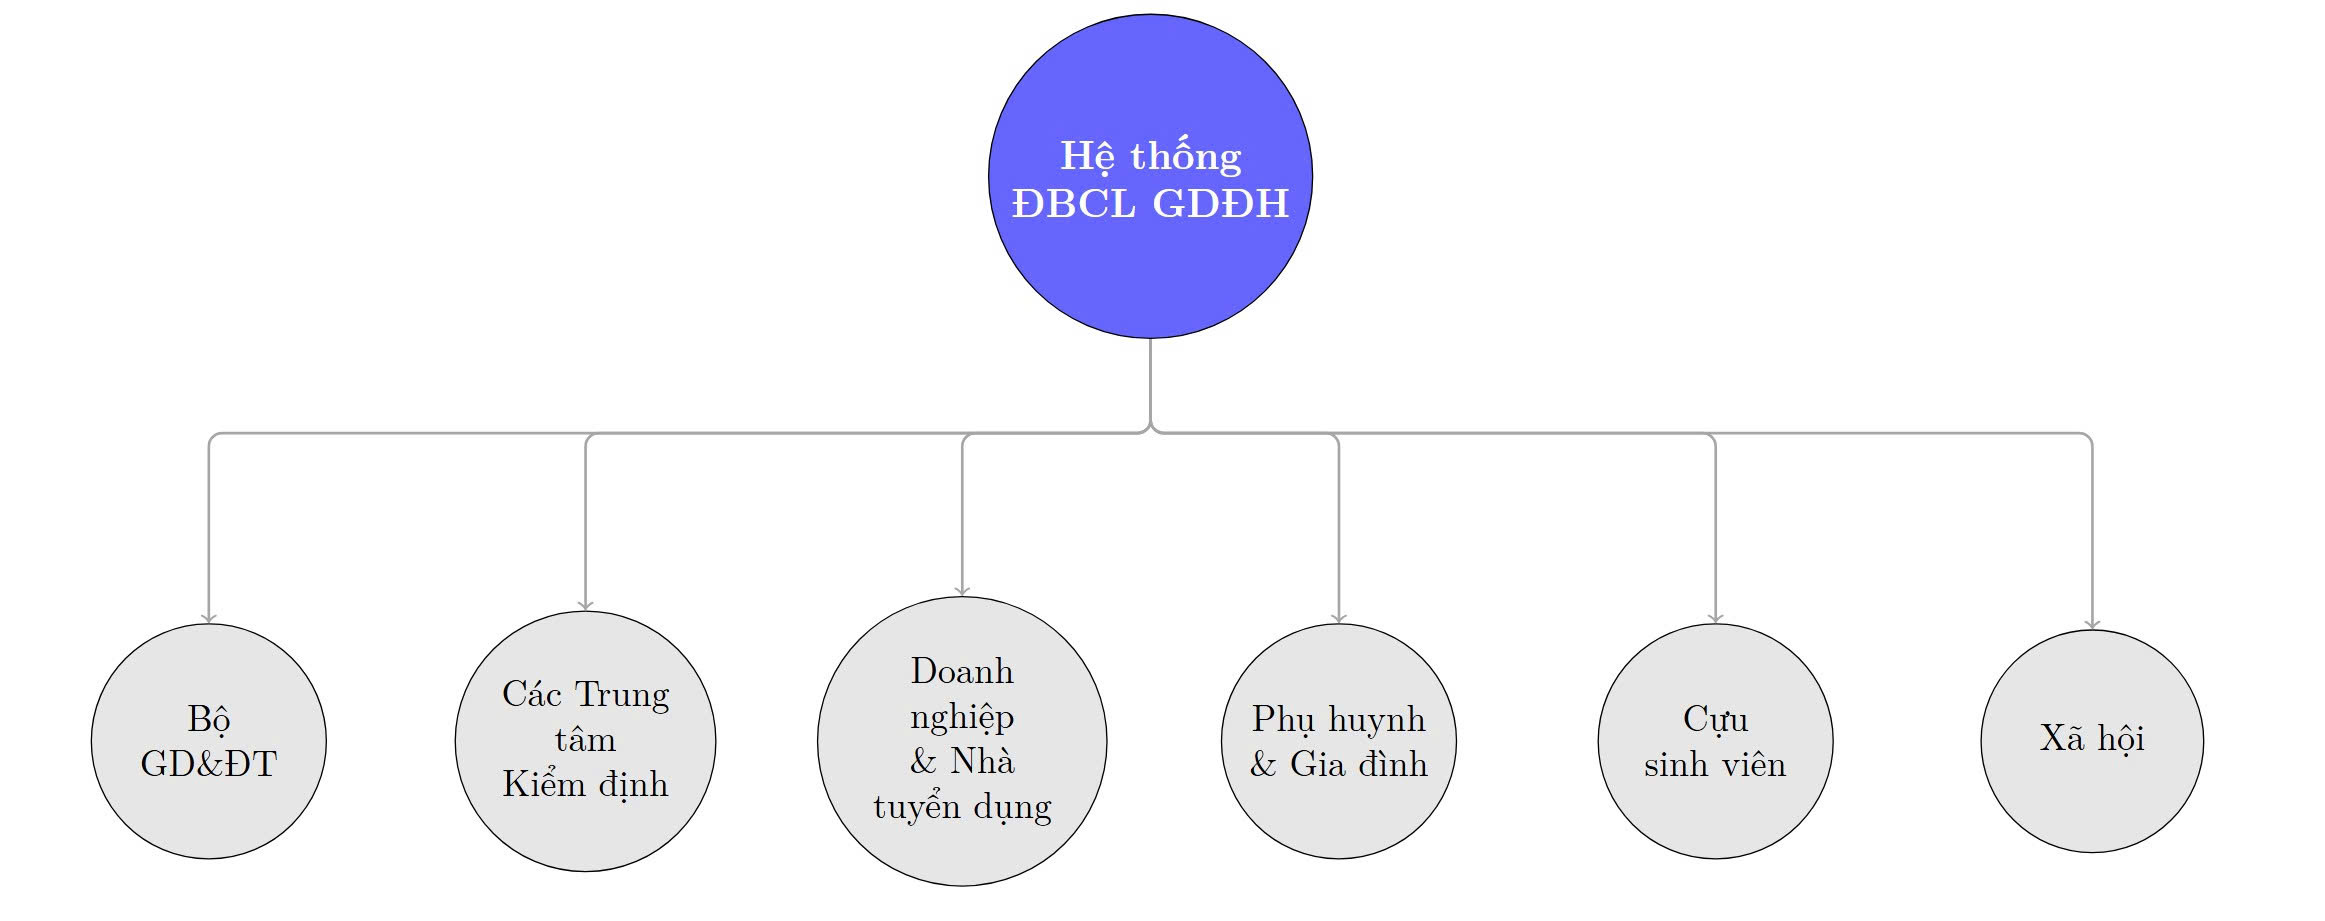
\includegraphics[width=\textwidth]{image/he_thong_dbcl_gddh.jpg}
    \caption{越南高等教育质量保障体系中的主要利益相关者图}
    \label{fig:so_do_he_thong_dbcl}
\end{figure}

上图可分为两大主要群体:
\begin{enumerate}
    \item \textbf{管理与执行群体(左侧与中心):} 包括国家机构和被直接授权的组织,扮演着制定政策和执行认证活动的角色。该群体包括\textbf{教育培训部}和各\textbf{认证中心}。
    \item \textbf{监督与受益群体(右侧):} 包括社会中的各个主体,他们是高等教育“产品”的直接使用者,并为质量提供重要的反馈。该群体包括\textbf{企业与雇主}、\textbf{家长与家庭}、\textbf{校友},以及更广泛的整个\textbf{社会}。
\end{enumerate}
分析这些主体,特别是制定“游戏规则”的群体之间的角色和关系,将阐明正在塑造越南质量保障现状的动因和压力。

\subsection{教育培训部:游戏规则的制定者与合规性压力}
\label{subsec:vai_tro_moet}

在越南的质量保障生态系统中,教育培训部扮演着核心权力主体的角色,负责构建和协调整个体系。从委托代理理论的视角来看,教育培训部是最高的“委托人”,将培养和保障质量的任务委托给各大学(代理人)\footcite{Kivisto2008}。同时,根据新制度主义理论,该部是产生最强大“强制性压力”的源头,迫使各大学遵守一个共同的法规框架,以获得合法性并维持运作\footcite{MeyerPowell2020}。

这种引领作用通过颁布一系列法规文件得以清晰体现,其核心精神由关于“根本性、全面性教育与培训革新”的第29号决议所指导\footcite{nghi_quyet_29_2013}。该决议明确提出了“增强教育培训机构的自主权和社会责任”以及建立一个“独立的认证体系”的要求。正是这些战略性导向,构建了法律走廊,推动各大学逐步与区域及国际标准接轨。

然而,这种集中的垂直管理机制,虽然对于确保统一性是必要的,但也正是导致许多教育机构形成一种\textbf{“合规文化”}而非\textbf{“改进文化”}的根本原因之一\footcite{pham2021governance}。各大学,特别是严重依赖国家预算的公立大学,倾向于优先开展旨在满足该部的报告要求和认证标准的活动,有时会轻视来自内部的实质性改进。因此,教育培训部既扮演着“游戏规则”制定者的角色,又是最高监督者,创造了一个合规性通常被置于创新之上的制度环境。

\subsection{质量认证中心:政策执行与独立性问题}
\label{subsec:vai_tro_trungtamkd}

如果说教育培训部是“委托人”,那么各教育质量认证中心则扮演着重要的“代理人”角色,其任务是具体化和执行认证政策。这些中心体系的发展,是越南质量保障活动制度化努力的证明。截至2024年初,全国共有7家获准运营的教育质量认证中心,包括公立和私立单位\footcite{tuoitre_kdcl_stats_2024}。

该体系已积极运作,在执行国家质量政策方面扮演着重要的“延伸手臂”角色。截至2023年底,这些中心已对全国\textbf{1855个培养项目}和\textbf{187所教育机构}进行了认证和承认\footcite{tuoitre_kdcl_stats_2024}。2021年两家私立中心的成立,也标志着朝着社会化、评估单位多样化方向迈出了新的一步。

然而,学术界和管理层提出的一个重要问题是这些中心的\textbf{实质性独立性}。尽管是以独立法人身份成立,但7家中心中有5家仍是大型大学或协会的下属单位,并且所有中心都在教育培训部的严密监督下运作。这种“既是主管单位,又是被认证对象”的关系,可能会引起人们对评估结果绝对客观性的怀疑\footcite{giaoducnet_kdcl_list_2023}。更重要的是,它有可能会进一步强化大学的合规压力。许多学校并未将认证中心视为共同改进的伙伴,而是仍然抱着应付上级“检查”的心态。这种复杂的关系将在后续章节中,在审视质量文化和体系协调等挑战时进行更深入的分析。


% het goi 3




\section{基于V-AQA模型的现状分析}
\label{sec:phan_tich_vqa}

在确定了主要主体的角色和体系的“游戏规则”之后,本章将运用V-AQA模型的五个要素,系统地“解剖”越南高等教育质量保障体系所面临的核心挑战。分析将从问题的源头——领导能力和组织文化——这两个具有紧密因果关系并塑造校内所有质量活动的要素开始。

\subsection{要素一:领导与治理的挑战——自主与合规之间}
\label{subsec:thach_thuc_lanhdao}

\textbf{领导与治理}要素是整个质量保障体系的发起、导向和提供能量的源泉。它体现在高层领导团队(校董会、校领导班子)在战略上引领学校实现质量目标的愿景、承诺和能力。然而,在越南,这一领导角色正处于两难境地,被困在推动自主的政策和仍然带有浓厚合规性的管理实践之间。

\subsubsection{自主政策与管理实践的矛盾}
尽管大学自主的主张已在修订后的《高等教育法》中制度化,但在实际推行中仍存在诸多障碍。顶尖专家已指出规定与实践之间的严重不匹配。根据顶尖高等教育政策专家之一\textbf{范氏丽博士}的分析,现行大学自主的法律框架如同“一件遮不住身体的紧身衣”\footcite{lypham_aosat_2024}。她论证道,“主管部门”的概念仍然是一个巨大的障碍,这种理解与国际惯例相去甚远,削弱了自主的本质。公立大学倾向于只向管理层“报告”,而不是真正地对社会就培养质量负责,这使得问责制变得形式化。

同样,前高等教育司副司长\textbf{黎曰劝博士}也提出了一个坦率的看法:“不废除主管部门机制,就别急着转向自主”\footcite{khuyen_bochuquan_2022}。他分析称,只要主管部门还存在并有权干预人事和财务决策,校董会的实质性自主权就会受到限制。届时,学校领导者的角色很难摆脱行政命令执行者的地位,而不是成为一个真正的战略管理者。

\subsubsection{后果:领导层优先级的转移}
这种情况的直接后果是,领导团队在质量方面的战略管理能力未能得到充分发挥。许多管理者不得不将大部分时间和精力用于处理行政程序和满足上级要求,而不是能够专注于制定长期决策,如建设质量文化、推动创新或建立战略联盟。他们的重心从“如何实质性、可持续地提升质量?”这一问题,转移到更短期的“如何完成报告并通过认证评估?”这一问题上。这种优先级的转变是一个无形但极其强大的障碍,它抑制了来自基层的创新努力,并直接催生了下文将分析的应付式质量文化。

\subsection{要素二:质量文化的挑战——从被动合规到主动改进}
\label{subsec:thach_thuc_vanhoa}

如果说领导与治理要素是质量保障体系的“大脑”,那么\textbf{质量文化}就是其“灵魂”,是决定质量流程是得到实质性执行还是仅为形式应付的关键因素。哈维和斯坦塞克(2008)将质量文化定义为一个共享的价值观和信念集合,组织中的每个成员都自觉地致力于持续改进\footcite{HarveyStensaker2008}。然而,实践证据表明,这是越南高等教育中最重大且固有的挑战之一,是上述带有浓厚合规性管理模式的直接后果。

\subsubsection{“反应型质量文化”的定性}
一项关于越南大学质量文化的深入研究,将这一特征定性为一种\textbf{“反应型质量文化”}。在此层次上,组织仅在出现问题或有外部压力(例如:认证评估)时才关注质量,而不是主动寻找改进机会\footcite{vjol_reactiveculture_2021}。质量保障活动通常只在认证周期临近时才被大力推动,并在学校获得证书后趋于“沉寂”。这是质量保障研究中常称的“季节性活动”或“认证风暴”现象。

从新制度主义理论的角度看,这是“脱钩”现象的典型表现,即组织形式上采纳所要求的结构和流程以获得合法性,而内部核心活动(教学、学习、研究)却无实质性改变\footcite{MeyerRowan1977}。这种文化的直接后果是学术团队的被动参与。本应是改进过程主体的教师和员工,却常常将质量保障活动视为一种行政负担,一种教学专业之外的“额外工作”\footcite{iosr_passiveparticipation_2021}。

\subsubsection{通过社会信任的波动表现出来}
内在质量文化的脆弱性必然会通过社会的信任度反映出来,而考生和家庭的入学决定是一个敏感指标。图\ref{fig:ty_le_nhap_hoc}显示了2015-2024年间考生确认入学比例的显著波动。

\begin{figure}[h!]
    \centering
    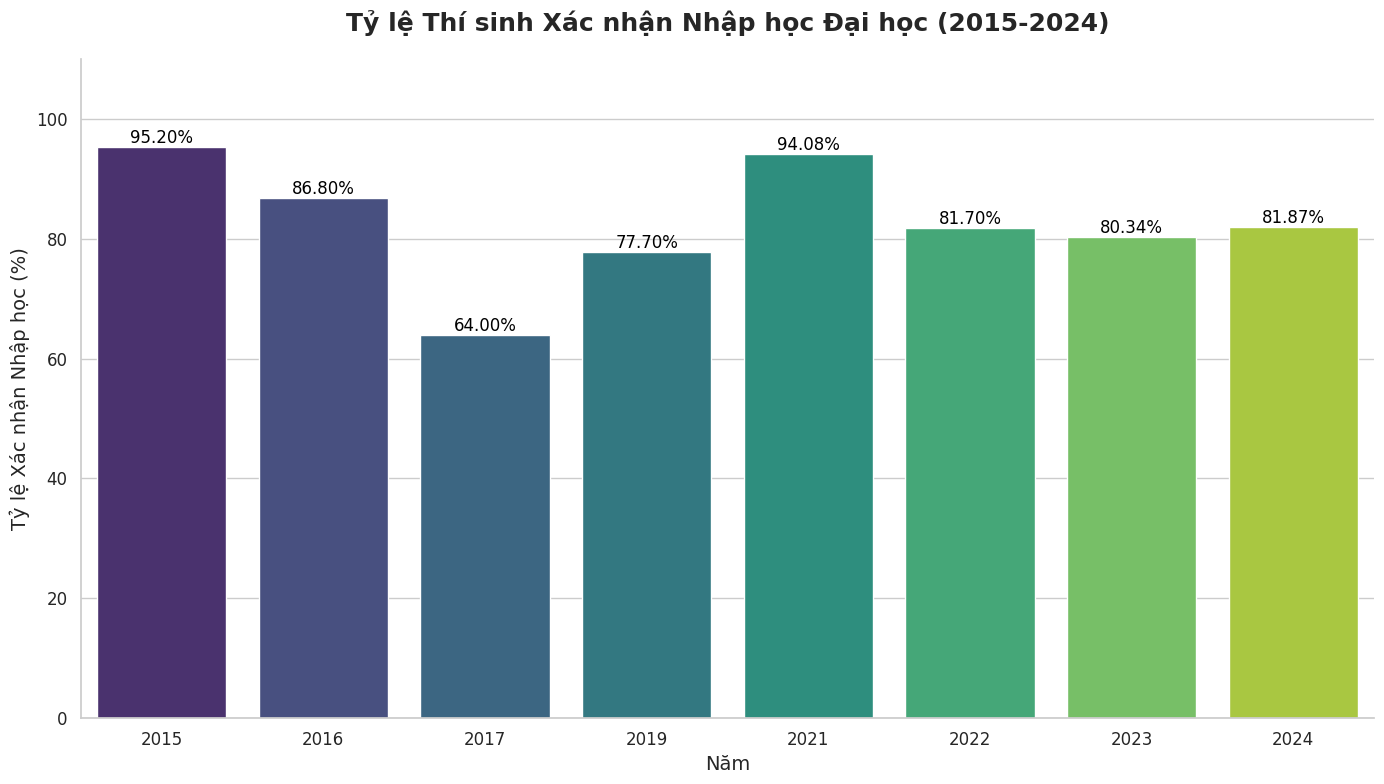
\includegraphics[width=\textwidth]{image/ty_le_nhap_hoc_2015-2024.png}
    \caption{大学新生确认入学比例(2015-2024年)}
    \label{fig:ty_le_nhap_hoc}
    \vspace{0.2cm}
    \footnotesize{\textit{来源:综合整理自教育培训部历年招生数据。}}
\end{figure}

图表并未呈现稳定的增长趋势,而是显示出剧烈波动。特别是,从2016年的86.8\%急剧下降到\textbf{2017年的仅64\%},是一个令人警醒的信号。这种突降不能仅用招生规定的变化来解释,更可以被解读为当时社会对大学文凭价值和质量的一次“信任危机”,此前媒体已长期广泛报道本科生失业问题。

近年来该比例的回升并维持在较高水平(80%以上),显示了整个体系的改进努力,尤其是在修订后的《高等教育法》生效之后。然而,正是这种波动表明,利益相关者的信任仍然脆弱,越南高等教育的感知质量尚未真正稳固。一个实质性的、来自内部的质量文化,需要创造一个稳定可靠的承诺,而不是像这样充满波动且依赖外部因素的结果。

\subsubsection{打破惰性的努力:促进机制的案例研究}
尽管合规文化仍然普遍,但一些教育机构已开始率先采用具体的治理机制来打破这种惰性。一个典型案例是\textbf{胡志明市技术大学}。自2022年起,该校推行了一项具有杠杆作用的政策:学生必须完成关于教师教学活动的在线调查,才能查看该课程的期末考试成绩\footcite{hutech_khao_sat_2022}。
这项政策创造了一个积极而强大的反馈循环。学生完成调查问卷的比例达到非常高的平均水平,提供了一个巨大而全面的反馈数据源。面对这些数据,教师被迫倾听并参与到改进过程中。结果显示,许多教师已主动调整方法、更新课件幻灯片并补充实践案例。这个案例生动地说明,质量文化并非一个抽象概念,而是可以通过足够强大的具体治理机制来影响和塑造,从而从被动参与转变为主动调整。


% het goi 4























	% 

\chapter{为越南高等教育提出混合与适应性质量保障模型(V-AQA模型)}
\label{chap:de_xuat_vqa}

\section[引言]{引言:背景与新模型的紧迫性}
\addcontentsline{toc}{section}{引言}

基于第三章对越南高等教育质量保障体系现状及其系统性挑战的深入分析,得出了一个重要结论:现存问题之间存在因果联系,形成了复杂的“恶性循环”。世界银行的诊断报告已明确指出治理薄弱、培养与市场脱节以及质量保障体系尚未真正有效等问题\footcite{worldbank_improvingperformance}。这些问题并非孤立存在,而是相互交织,包括:大学自主权仍然有限\footcite{world-bank_improvingperformance},利益相关者参与度不高\footcite{pmc_article_9127449},质量文化带有浓厚的应付色彩\footcite{vjol_reactiveculture},以及质量保障人力资源既缺又弱\footcite{pmc_article_9127449}。

这表明,采用零散、片面的解决方案或机械地照搬国外的传统模式,将无法从根本上解决问题。越南需要一种新的方法,一个全面的行动框架,既能适应一个转型期经济体的特殊背景,又能与国际质量标准接轨。

为响应这一要求,本章将提出并详细论证一个新模型——\textbf{混合与适应性质量保障模型(简称V-AQA)}。该模型不仅是一系列孤立解决方案的集合,更是一个系统的思维和行动框架,旨在直接打破已指出的“恶性循环”,并从内部推动一种可持续的质量文化。

\section{越南现行质量保障框架的差距分析}
\label{sec:phan_tich_khoang_trong}

为申明V-AQA模型的紧迫性和适用性,首先需要分析在越南普遍应用的现有质量保障框架未能彻底解决的差距。

\subsection{东盟大学网络质量保障标准}

东盟大学网络及其质量保障标准在推动质量文化和区域一体化方面做出了巨大贡献。

\paragraph{优势} 东盟大学网络质量保障提供了一套全面的标准(4.0版共8项标准),重点关注成果导向教育和以学习者为中心\footcite{AUN-QAGuide}。获得东盟大学网络质量保障标准认证有助于越南的培养项目提升声誉,并为区域内的学生交换和学分互认创造便利条件\footcite{hoasen_benefits_aunqa}。

\paragraph{差距与局限}
\begin{itemize}
    \item \textbf{主要集中于课程层面:} 尽管有机构层面的标准,但在越南应用东盟大学网络质量保障标准主要发生在课程层面。这可能导致质量不均衡的状况,即少数几个项目达到国际标准,而整个机构,特别是在治理和资源分配方面,仍然沿用旧模式\footcite{aun_institutional_v2}。
    \item \textbf{流程复杂且成本高昂:} 寻求东盟大学网络质量保障认证需要大量的财政和人力资源,这为许多学校,特别是民办或地方院校设置了障碍\footcite{stdjssh_637}。
    \item \textbf{“形式化合规”的风险:} 获得认证的压力可能导致学校专注于完善档案和证据,以机械地满足标准,而不是从内部推动实质性改进\footcite{pmc_article_9127449}。
\end{itemize}

\subsection{教育培训部的规定}
教育培训部的法规文件体系,特别是关于质量认证的通知(如基于东盟大学网络质量保障标准制定的第12/2017号通知),为质量保障活动创造了强制性的法律走廊。

\paragraph{优势} 教育培训部的规定在整个体系内设立了最低质量要求,迫使教育机构进行自评和外部认证,有助于提升对质量保障的普遍认识。

\paragraph{差距与局限}
\begin{itemize}
    \item \textbf{体系缺乏独立性:} 各教育质量认证中心仍受教育培训部的直接管理,这引发了关于国家管理机构与专业认证机构之间客观性和独立性的担忧\footcite{ncdt_journal_219}。
    \item \textbf{大学自主权仍然有限:} 尽管自主政策已经颁布,但执行中仍存在诸多障碍。根据世界银行的报告,只有一小部分公立大学真正参与了自主试点,且自主范围仍然狭窄,特别是在组织和人事方面\footcite{world-bank_improvingperformance}。这降低了学校根据自身需求灵活改进质量的能力。
    \item \textbf{合规文化:} 按照教育培训部规定进行的认证通常被视为一项必须完成的行政义务,导致了“应付式合规”文化,而非内在的改进需求\footcite{vjol_reactiveculture}。
\end{itemize}

\subsection{构思-设计-实现-运作能力框架}
构思-设计-实现-运作是一个先进的框架,被越南许多工科院校采用,以改革培养方案,使其满足企业要求。

\paragraph{优势} 构思-设计-实现-运作提供了一个集成的学习框架,将理论与实践相结合,帮助学生全面发展个人、沟通和专业技能。应用构思-设计-实现-运作极大地推动了工科院校教学方法的创新\footcite{vietnamplus_cdio_reform}。

\paragraph{差距与局限}
\begin{itemize}
    \item \textbf{范围狭窄且难以推广:} 构思-设计-实现-运作主要为工程和技术学科设计。将该模型应用于社会科学、经济学或师范等学科是一个巨大挑战。
    \item \textbf{要求深刻的文化变革:} 成功实施构思-设计-实现-运作要求在思维和组织文化上发生重大变革,从领导层到每一位教师。在越南的研究已指出这种变革的困难,包括初期领导层缺乏正式承诺以及核心教师团队与其余人员之间互动有限\footcite{nguyen_cdio_2016}。
\end{itemize}

\section{V-AQA模型的定位:比较优势与优越性}
\label{sec:dinh_vi_vqa}

基于对上述差距的分析,提出V-AQA模型并非旨在完全替代,而是为了整合并克服现有框架在越南特殊背景下未能彻底解决的固有弱点。

与这些模型相比,V-AQA拥有突出的优势:
\begin{itemize}
    \item \textbf{混合性:} 主动平衡来自外部的\textbf{问责制}压力(教育培训部的要求)和来自内部的\textbf{持续改进}动力(东盟大学网络质量保障和构思-设计-实现-运作的精神),而不是只关注一个方面。
    \item \textbf{适应性:} 按照灵活的短期改进周期运作,帮助学校快速响应市场变化,而不是遵循僵化的长期计划。
    \item \textbf{全面性与内生性:} 作用于学校的全部五个核心方面(领导与治理、文化、利益相关者、流程、合作),并推动来自内部的变革(内生性),而不仅仅是遵守外部要求。
    \item \textbf{技术整合性:} 以管理信息系统为“神经系统”,使基于证据的治理成为可能,这是其他框架未直接提及的因素。
\end{itemize}

为更清晰地说明这种差异,下表将V-AQA与越南普遍应用的框架进行对比:

\begin{table}[h!]
\centering
\caption{V-AQA模型与普遍应用框架的对比表}
\label{tab:doi_sanh_vqa}
\begin{tabular}{|p{3cm}|p{3.5cm}|p{3.5cm}|p{3.5cm}|}
\hline
\textbf{比较标准} & \textbf{东盟大学网络质量保障(课程层面)} & \textbf{教育培训部规定(第12号通知)} & \textbf{V-AQA模型(建议)} \\
\hline
\textbf{主要目标} & 根据东盟共同标准评估、比对课程质量。 & 为各校规定最低标准和强制性认证流程。 & \textbf{从内部创建一个全面、自我改进且可持续的质量体系。} \\
\hline
\textbf{应用范围} & 主要在培养课程层面。 & 课程层面和教育机构层面。 & \textbf{全面覆盖学校层面,从领导、文化到每一个流程。} \\
\hline
\textbf{自主程度} & 学校自愿参加,但必须严格遵守东盟大学网络流程。 & 低,认证机构仍依赖教育培训部,合规性强\footcite{ncdt_journal_219}。 & \textbf{高且有导向:推动自主与通过关键绩效指标明确问责相结合。} \\
\hline
\textbf{利益相关者参与} & 有提及,但实际上学生和企业参与仍然有限\footcite{pmc_article_9127449}。 & 咨询性质,缺乏实质性约束机制。 & \textbf{将利益相关者的角色机制化(行业咨询委员会、学术委员会中的学生代表)。} \\
\hline
\textbf{灵活性} & 标准化流程,灵活性低。 & 规定具有普遍适用性,较为僵化。 & \textbf{高,是核心原则(适应性),允许根据短期周期进行调整。} \\
\hline
\end{tabular}
\end{table}

\textit{(注:构思-设计-实现-运作能力框架未直接纳入比较表,因为其本质是针对工科领域的专门培养方案开发框架,与东盟大学网络质量保障和教育培训部规定的综合性质量保障体系性质不同)。}

上表显示,V-AQA不仅是一套标准,更是一个\textbf{治理框架}。V-AQA不只关注“需要达成什么”,更关注“如何”构建一个能够自我改进的组织。这种方法直接解决了自主、质量文化和利益相关者参与等基础性问题,而仅仅应用单一标准是无法触及这些问题的。

为更深入地理解塑造这些比较优势的思想基础,下一部分将深入论证V-AQA模型的混合理念与适应性原则。


% het goi 1


\section{V-AQA模型的哲学基础与原则}
\label{sec:triet_ly_nguyen_tac_vqa}

V-AQA模型建立在两大哲学基础上,这两大基础是从国际研究和对越南特殊背景的分析中总结出来的:混合哲学与适应性原则。这正是该模型的“灵魂”,塑造了其所提出的方法和解决方案。

\subsection{混合哲学:协调问责制与质量改进}

越南高等教育体系目前正承受着双重压力。一方面,由于国家的主导作用和对公共预算的依赖,各大学必须强有力地满足\textbf{问责制}的要求。另一方面,在日益激烈的竞争和劳动力市场要求的背景下,各大学又迫切需要进行\textbf{改进}以提升质量和品牌。

这两个目标常常产生矛盾,导致要么过分注重形式上的合规以满足外部要求,要么是自发、无纪律的内部改进。V-AQA模型的“混合”哲学正是为了解决这种紧张关系而提出的。正如哈维和威廉姆斯(2010)在对高等教育质量十五年的综述中所分析的,一个有效的体系必须设法整合并协调这两个目标\footcite{harvey_williams_2010}。V-AQA模型通过承认外部透明的问责要求可以为推动内部改进努力提供必要的数据和压力来实现这一点。反之,强大的改进文化将使学校更容易满足并超越问责要求。这种方法有助于将关系从对抗转为共生,其中遵守规定成为前提,而提升质量成为最终目标。

\subsection{适应性原则:在变化背景下的灵活性}

越南的经济社会和政策背景正在以极快的速度变化。第四次工业革命、关于大学自主的新政策以及劳动力市场的波动,都要求质量保障体系必须具有高度的灵活性。一个为期五年的僵化质量改进计划,有可能在尚未执行完毕时就已经过时。

因此,V-AQA模型建立在“适应性”原则之上,其灵感来自于像适应性项目框架这样的敏捷项目管理框架\footcite{Wysocki2009}。该原则鼓励采用短期的、重复的改进周期,而不是一个长期的PDCA循环。各学校可以按学年甚至学期设定质量目标,实施、快速收集反馈数据,并为下一个周期调整计划。这种方法帮助各学校“边做边学”,最大限度地减少长期错误决策的风险,并确保改进努力始终与不断变化的实际背景相符。

\section{V-AQA模型的总体结构与要素}
\label{sec:cau_truc_tong_the}

基于上述两大哲学基础,V-AQA模型被建构为一个由理论基础、五个相互作用的核心要素和最终目标组成的总体结构。

\begin{figure}[h!]
    \centering
    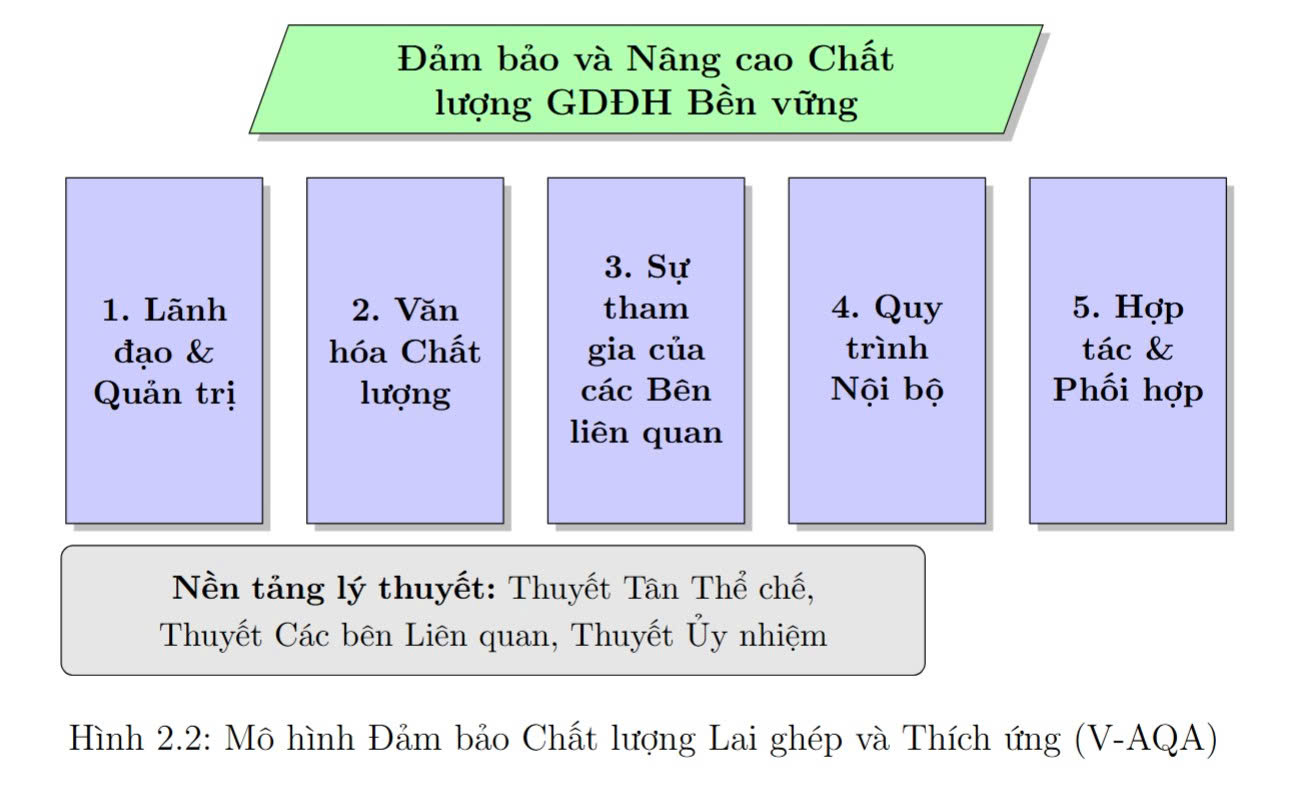
\includegraphics[width=\textwidth]{image/mo_hinh_V-AQA.jpg}
    \caption{混合与适应性质量保障模型 (V-AQA)}
    \label{fig:v-aqa-model-detailed}
\end{figure}

V-AQA模型的五个要素相互作用,形成一个完整的质量体系。为给读者,特别是那些非质量保障领域的专业人士,提供一个全面且易于理解的概览,下表将总结每个要素的目标、具体表现以及建议的关键绩效指标。该表如同一张“地图”,为后续的详细分析部分勾画了结构。

\begin{longtable}{|p{2.5cm}|p{3.5cm}|p{4.5cm}|p{3.5cm}|}
\caption{V-AQA模型5要素总结}
\label{tab:tong_hop_5_thanh_to}\\
\hline
\textbf{要素} & \textbf{主要目标} & \textbf{具体表现(行动)} & \textbf{衡量方式(关键绩效指标示例) \footcite{uq_kpi_dashboard}} \\
\hline
\endfirsthead
\multicolumn{4}{c}%
{{\bfseries \tablename\ \thetable{} -- 续前页}} \\
\hline
\textbf{要素} & \textbf{主要目标} & \textbf{具体表现(行动)} & \textbf{衡量方式(关键绩效指标示例) \footcite{uq_kpi_dashboard}} \\
\hline
\endhead
\hline \multicolumn{4}{r}{{续下页}} \\
\endfoot
\hline
\endlastfoot

% 第1行
\textbf{1. 领导与治理} & 将领导者从“控制者”转变为“环境创造者”。 & 
\begin{itemize}
    \item 制定并执行校级质量战略。
    \item 向院系下放强有力的权力并辅以问责制。
    \item 为中层管理团队提供能力提升培训。
\end{itemize} & 
\begin{itemize}
    \item 质量战略中各项目标的完成率。
    \item 各院系对自主权的满意度。
    \item 完成现代治理培训的中层管理者数量。
\end{itemize} \\
\hline

% 第2行
\textbf{2. 质量文化} & 从“应付式合规”文化转变为“主动改进”文化。 & 
\begin{itemize}
    \item 发起系统的质量宣传运动。
    \item 建立表彰和奖励改进创举的体系。
    \item 成立并授权“质量改进小组”。
\end{itemize} & 
\begin{itemize}
    \item 关于质量文化认知的定期调查得分。
    \item 每年提出并实施的改进创举数量。
    \item 参与改进活动的教职工比例。
\end{itemize} \\
\hline

% 第3行
\textbf{3. 利益相关者的参与} & 将利益相关者(企业、学生、校友)转变为“战略伙伴”。 & 
\begin{itemize}
    \item 将行业咨询委员会的活动机制化。
    \item 让学生代表在科学与培养委员会中拥有投票权。
    \item 建立主动的“校友大使”网络。
\end{itemize} & 
\begin{itemize}
    \item 行业咨询委员会的建议被整合到培养方案中的比例。
    \item 有学生代表参与的学术决策数量。
    \item 企业对毕业生契合度的满意度得分。
\end{itemize} \\
\hline

% 第4行
\textbf{4. 内部流程} & 基于数据实现学术和管理流程的现代化、标准化。 & 
\begin{itemize}
    \item 采用基于成果导向教育理念的培养方案开发流程。
    \item 多样化教学和评估方法。
    \item 构建并整合质量保障管理信息系统。
\end{itemize} & 
\begin{itemize}
    \item 按照成果导向教育流程制定和审查的培养方案比例。
    \item 课程中过程性评估分数的平均比重。
    \item 基于质量保障管理信息系统数据做出的管理决策比例。
\end{itemize} \\
\hline

% 第5行
\textbf{5. 合作与协调} & 打破“孤岛”状态和封闭思维,创造一个开放的质量生态系统。 & 
\begin{itemize}
    \item 为跨学科、跨单位的质量改进项目提供经费。
    \item 建立并参与标杆比对网络。
    \item 战略性地利用国际认证活动进行学习。
\end{itemize} & 
\begin{itemize}
    \item 成功实施的跨院系/部门项目数量。
    \item 组织的标杆比对活动及产生改进报告的数量。
    \item 国际认证建议的完成比例。
\end{itemize} \\
\end{longtable}

本章的后续部分将深入分析和论证上述五个要素中的每一个,包括建议的解决方案、科学依据、潜在风险及缓解策略。



% het goi 2 chuong 4



\section{V-AQA模型的各要素与建议解决方案}
\label{sec:cac_thanh_to_vqa}

V-AQA模型由五个相互作用的要素构成,每个要素代表一组战略性解决方案,旨在解决第三章中已分析的挑战。接下来的部分将深入探讨每个要素,论证其建议的解决方案及其背后的科学与实践依据。

\subsection{要素一:以分权和责任为导向重构领导与治理}
\label{subsec:giaiphap_lanhdao}

如前所述,当前质量保障体系的最大障碍之一是领导角色带有浓厚的行政、合规色彩,且权力过于集中\footcite{vnujs_fs_4303}。因此,V-AQA模型的第一个要素聚焦于重构这一角色,目标是将领导者从“控制者”转变为质量文化的“环境创造者”和“推动者”\footcite{unesco_gem_report_2024}。

\paragraph{解决方案1.1:制定并执行校级质量战略。}
为摆脱季节性的应付状态,每所大学都需要制定一份正式的五年期\textbf{质量战略},并将其紧密融入学校的总体发展战略中。这并非一份形式化的文件,而是最高层领导的政治承诺。该战略必须回答以下核心问题:
\begin{enumerate}
    \item 学校从哪些维度定义“质量”(研究质量、教学质量、市场契合度、学生体验)?
    \item 未来五年的优先质量目标是什么,并以可衡量的关键绩效指标具体化?(例如:将学生就业率提高到95%,国际发表数量每年增加20%)。
    \item 将分配哪些资源(财政、人力、技术)来实现目标?
    \item 谁为每个具体目标负责(明确各处、室、院系的角色分工)?
\end{enumerate}
拥有一份清晰且广为宣传的战略,是有效和负责任地执行自主权的先决条件,正如教育培训部关于大学自主的报告所强调的\footcite{moet_report_autonomy}。

\paragraph{解决方案1.2:按“指导核心”模型进行分权并明确授权。}
基于委托代理理论\footcite{JensenMeckling1976},V-AQA模型提出了一种更强有力的分权机制,并辅以明确的问责制。学校需要从集权结构转向克拉克(1998)所分析的“指导核心”模型\footcite{clark_1998}。据此:
\begin{itemize}
    \item \textbf{校董会:} 专注于批准总体战略,监督战略目标的执行,并确保学校对社会的问责。
    \item \textbf{校领导班子:} 负责运营,制定支持性政策,并有效分配资源,以便各单位能够实现目标。
    \item \textbf{各院/系:} 必须在学术事务,如改进培养方案、创新教学方法和开展研究活动等方面,被赋予实质性的自主权。
\end{itemize}
这种自主权必须与一个清晰透明的关键绩效指标体系相结合。校领导班子使用该体系(通过质量保障管理信息系统上的仪表盘)来监督成效,而无需对具体的专业活动进行微观干预,这符合“远程指导”的精神。

\paragraph{解决方案1.3:提升中层管理团队的能力。}
一个好的战略无法由一个薄弱的管理团队来执行。因此,V-AQA模型强调投资于中层管理团队(院/系主任、副主任)能力的必要性。需要设计强制性的培训项目,不仅涉及行政业务,还包括现代大学治理技能,如:
\begin{itemize}
    \item 变革管理
    \item 战略思维与规划
    \item 数据驱动决策
    \item 激励型领导力
\end{itemize}
政府的\textbf{89号提案}等海外博士师资培训项目,应被利用并扩展,以包括为潜在管理者提供关于大学治理的培训和进修项目\footcite{moet_project_89}。这是对“人力资本”的投资,以确保改革从根本上取得成功。

\subsection{领导与治理要素的风险分析与缓解方案}
\label{subsec:risk_lanhdao}
重构领导与治理角色总是潜藏着重大风险。识别并制定预防这些风险的策略是确保成功的关键。

\begin{itemize}
    \item \textbf{风险1:高层领导的承诺浮于表面。}
    \textit{表现:} 领导可能在文件上支持改革,但行动上并不坚决,不提供足够资源,或在遇到困难时轻易改变优先事项。
    \textit{缓解策略:}
    \begin{itemize}
        \item 成立一个由校长或常务副校长直接担任组长的\textbf{质量改革指导委员会},有定期的会议日程和公开的报告。
        \item 为\textbf{校领导班子和各单位领导制定并颁布关键绩效指标},其中执行质量战略的指标在年终评优奖励中占有重要比重。
    \end{itemize}

    \item \textbf{风险2:来自中层管理的抵制。}
    \textit{表现:} 院系主任、处长可能会觉得在一个更透明的体系下运作会失去权力。他们可能会通过不合作、拖延实施或提供不准确的数据来进行暗中抵制。
    \textit{缓解策略:}
    \begin{itemize}
        \item 为100%的中层管理干部组织关于\textbf{变革管理和数据驱动治理的强制性培训},使他们清楚理解新模型的益处。
        \item \textbf{授权与赋能并行。} 当一个院系被分配了更高的关键绩效指标时,也必须在财务和人事方面赋予其相应的自主权,以便能够完成任务。
        \item \textbf{沟通与倾听:} 组织校领导班子与中层管理之间的定期对话会,倾听困难并共同寻找解决方案,而不是单向命令。
    \end{itemize}

    \item \textbf{风险3:分权但无法控制成效。}
    \textit{表现:} 过度下放自主权而没有一个有效的监督体系,可能导致院/系运作偏离方向,无法为学校的总体目标做出贡献。
    \textit{缓解策略:}
    \begin{itemize}
        \item \textbf{部署质量保障管理信息系统是先决条件。} 如果没有一个足够强大的信息系统来为校领导班子提供及时准确的数据,就无法进行分权。
        \item 建立一个\textbf{自上而下统一的、清晰的关键绩效指标体系},确保院/系/处室级别的指标都旨在实现校级战略指标。
    \end{itemize}
\end{itemize}

通过预见并主动管理上述风险,领导与治理要素可以成为强大的动力,而不是障碍,推动整个质量改革进程。


% het goi 3



\subsection{要素二:从合规文化向改进文化的转型}
\label{subsec:giaiphap_vanhoa}

“反应型质量文化”的挑战——即质量保障活动仅为应对外部认证要求而进行——已被确定为阻碍越南大学实质性质量提升的最大障碍之一\footcite{vjol_reactiveculture}。因此,V--AQA模型的第二个要素聚焦于制定战略性解决方案,以创造一个环境,使质量改进成为组织内从领导到员工每个成员的内在需求和日常习惯。

\paragraph{解决方案2.1:基于欧洲大学协会能力框架发起质量文化建设运动。}
文化不能靠命令创造,而必须通过共识和共享价值观来培育。V--AQA模型建议各大学基于\textbf{欧洲大学协会的质量文化框架},开展系统的宣传和意识提升运动\footcite{eua_quality_culture}。根据该能力框架,质量文化建立在机构层面和个人层面因素的互动之上。
\begin{itemize}
    \item \textbf{在机构层面:} 学校领导必须率先垂范,不断宣传质量的愿景、定义和重要性。关于质量的核心价值观必须被整合到发展战略、政策文件和学校的运作流程中。
    \item \textbf{在个人层面:} 运动需要侧重于提升每位教师、员工的意识、态度和能力。具体活动包括:组织研讨会、关于质量思维的培训课程,以及为坦诚对话质量改进中的障碍与机遇而设的开放论坛。
\end{itemize}
该运动的目标是让所有成员明白,质量不仅是质量保障部门的责任,而是每个人的责任。

\paragraph{解决方案2.2:建立改进创举的表彰与奖励体系。}
要将认知转化为行动,需要有实际的激励。V--AQA模型建议建立一个正式的表彰与奖励体系,以嘉奖质量改进的努力。正如哈维和威廉姆斯(2010)所指出的,创建激励机制是维持质量活动的重要组成部分\footcite{harvey_williams_2010}。具体而言,学校可以:
\begin{itemize}
    \item \textbf{设立年度奖项:} “教学创新年度教师奖”、“高效质量保障模式院系奖”、“最佳质量改进创举奖”。这些奖项需要有足够大的物质和精神价值以产生吸引力。
    \item \textbf{融入职业评估与发展流程:} 对质量改进的贡献标准必须被正式纳入年终干部、教师的评估、评级和评优奖励流程中。在规划、任命干部或考虑提前晋升时,这是一个重要的考量因素。
    \item \textbf{公开表彰:} 取得优异成绩的个人和集体需要在学校的宣传渠道(网站、简报、社交媒体)上隆重表彰,以传播良好榜样。
\end{itemize}
这些行动将发出一个强有力的信息:学校真正重视并奖励改进的努力,而不仅仅是看重完成行政任务。

\paragraph{解决方案2.3:通过“改进小组”为教师赋能并建设其能力。}
质量文化必须从基层建立。为解决教师“被动参与”的状况\footcite{iosr_passiveparticipation},V--AQA模型建议授权并创造条件,让他们成为改进过程的主体。具体解决方案是在系或院层面成立\textbf{“质量圈”}。这些是由自愿参加的教师组成的小组,任务是定期讨论教学、研究中的质量问题并提出解决方案。学校需要为这些小组提供小额预算(创举支持基金),以便他们可以试验新的教学方法、开发创新学习材料或组织专业研讨会。这种授权和资源提供将促进一种主人翁精神,将教师从被管理者转变为质量的创造者。

\subsection{质量文化要素的风险分析与缓解方案}
\label{subsec:risk_vanhoa}
改变组织文化是最困难和最长期的挑战之一。实施上述解决方案可能会面临以下风险:

\begin{itemize}
    \item \textbf{风险1:团队的惰性和怀疑态度。}
    \textit{表现:} 教师、员工已习惯于旧的工作方式,认为各种运动和活动只是形式主义,“雷声大雨点小”。他们可能会不情愿地参与,并且不相信会发生实质性变化。
    \textit{缓解策略:}
    \begin{itemize}
        \item \textbf{领导的模范作用:} 领导必须率先参与所有活动,从研讨会到提出创举。领导的行动比任何言语都更有说服力。
        \item \textbf{专注于“速赢”:} 在初期阶段,需要集中支持小型改进小组,以创造出积极、可见的成果。广泛宣传并奖励这些初步成功,将为改革过程创造动力并巩固信心\footcite{kotter_leading_change}。
    \end{itemize}

    \item \textbf{风险2:奖励体系不公平或吸引力不足。}
    \textit{表现:} 奖励评审过程不透明,带有主观性,或者奖励过小,无法产生真正的激励。这可能适得其反,造成不满和嫉妒。
    \textit{缓解策略:}
    \begin{itemize}
        \item \textbf{建立清晰、公开的创举评估标准:} 标准需要能够衡量创举对提升质量的影响(例如:改善学生学习成果,缩短手续办理时间)。
        \item \textbf{多样化奖励形式:} 除了财务奖励,还需要有其他形式的认可,如参加国际培训的机会,在职称评定中优先考虑,或在学校重大活动中获得表彰。
    \end{itemize}

    \item \textbf{风险3:“改进小组”运作效率低下。}
    \textit{表现:} 小组成立后没有实质性活动,只是形式上的会议,或者小组的建议未得到上级的倾听和支持。
    \textit{缓解策略:}
    \begin{itemize}
        \item \textbf{提供必要的资源和支持:} 学校需要设立一个申请和拨付流程简单的“创举支持基金”。同时,需要有一个单位(例如:质量保障处)扮演协调角色,为各小组提供专业支持。
        \item \textbf{建立正式的反馈机制:} 必须有一个清晰的流程,让院/校领导倾听并回应来自改进小组的建议。建议被认真考虑并付诸实施,将是小组继续运作的最大动力。
    \end{itemize}
\end{itemize}

建设质量文化是一场马拉松,而不是短跑。它需要学校各级人员的毅力、一致性和真正的承诺。

% het goi 4 chuong 4



\subsection{要素三:将利益相关者转变为战略伙伴}
\label{subsec:giaiphap_lienquan}

第三章已指出,越南质量保障体系的固有弱点之一是与利益相关者,特别是企业界和学习者本身,缺乏实质性联系\footcite{worldbank_improvingperformance}。这种关系通常停留在形式化、被动的层面,如单向的咨询活动或影响甚微的调查\footcite{vnujs_er_3848}。V-AQA模型的第三个要素提出了旨在打破学校与社会之间“壁垒”的解决方案,将关系从“形式化咨询”转变为“战略合作”。

\paragraph{解决方案3.1:通过咨询委员会将校企联系机制化。}
为使与企业的合作不再依赖于少数领导的个人关系或季节性活动,V-AQA模型提出了一个制度性解决方案:为每个专业或专业群成立并运作\textbf{行业咨询委员会}。这是在东盟大学网络质量保障或ABET等权威国际认证标准中的一项核心要求,这些标准强调利益相关者在设计和改进培养方案中的中心作用\footcite{aunqa_guidelines_v4}。

行业咨询委员会的作用不仅限于参加研讨会。其运作章程需要明确制定,规定具体且具有约束力的任务:
\begin{itemize}
    \item \textbf{审定预期学习成果:} 行业咨询委员会负责审定并对专业院系制定的预期学习成果提出建议,确保其真实反映劳动力市场当前和未来的能力要求(知识、技能、态度)。
    \item \textbf{为培养方案提供定期建议:} 每年至少一次,专业院系必须向行业咨询委员会提交培养方案的审查报告,以获取关于技术、软技能和行业新趋势的更新建议。这些建议必须被记录并有相应的回应计划。
    \item \textbf{参与学术活动:} 邀请行业咨询委员会成员参与毕业设计答辩委员会;在专业课程中担任客座讲师;或为学生提出实际的项目课题。
\end{itemize}
这种机制化将创造一个可持续的对话与合作渠道,确保培养方案始终“跟上”实践,解决培养与市场“不匹配”的问题\footcite{worldbank_improvingperformance}。

\paragraph{解决方案3.2:提升学生和校友的角色。}
除了企业,学生和校友是对一个培养方案质量有最深刻见解的利益相关者。然而,他们通常被视为质量保障体系中的被动对象\footcite{pmc_article_9127449}。V-AQA模型基于阿恩斯坦的“参与阶梯”精神,提出了将他们的角色从被调查对象提升为真正合作伙伴的解决方案\footcite{Arnstein1969}。
\begin{itemize}
    \item \textbf{为学生赋权:} 学生代表(通过民主方式选举产生)不应只参与活动性组织,而应在像院级科学与培养委员会这样的学术性委员会中拥有一个带有\textbf{投票权}的正式席位。这确保了学习者的声音在关于课程、教学方法和学生支持政策等重要决策中得到认真考虑。
    \item \textbf{建立主动的校友网络:} 为每个专业建立一个\textbf{“校友大使”}体系。这些是事业有成且热心的校友,被正式邀请参与为低年级学生提供咨询和职业指导。更重要的是,他们将是定期提供关于培养方案在实际工作中的契合度的结构化反馈的来源。来自学生就业调查的数据\footcite{moet_graduate_survey}将是该网络有效运作的重要输入。
\end{itemize}

\subsection{利益相关者要素的风险分析与缓解方案}
\label{subsec:risk_lienquan}
加强利益相关者的参与,尽管非常必要,但在实施过程中也面临不少风险。

\begin{itemize}
    \item \textbf{风险1:企业参与流于形式,不具实质性。}
    \textit{表现:} 行业咨询委员会成员可能因人情关系而接受邀请,但不花时间研究文件并提出肤浅的建议。他们将此视为一项“社交”活动而非专业责任。
    \textit{缓解策略:}
    \begin{itemize}
        \item \textbf{建立“双赢”关系:} 除了为社会做贡献,学校需要为企业创造实际利益,如:为他们的员工提供进修课程,提供招聘品牌宣传机会,或优先对接研究和技术转让项目。
        \item \textbf{谨慎选择行业咨询委员会成员:} 优先选择真正热心于教育、具有深厚专业知识并愿意承诺时间的专家。行业咨询委员会的运作章程需要有替换不活跃成员的条款。
    \end{itemize}

    \item \textbf{风险2:学生代表的冷漠或能力不足。}
    \textit{表现:} 学生被赋予权力但因胆怯、缺乏批判性思维能力或未被提供足够信息以提出建设性意见而不发言。
    \textit{缓解策略:}
    \begin{itemize}
        \item \textbf{为学生代表组织技能培训课程:} 在参加委员会之前,学生代表需要接受关于批判性思维、如何阅读和分析政策文件以及有效沟通技巧的培训。
        \item \textbf{充分、及时地提供信息:} 委员会会议的材料必须在合理的时间前发送给学生代表,以便他们可以研究并收集其他学生的意见。
    \end{itemize}

    \item \textbf{风险3:利益和观点的冲突。}
    \textit{表现:} 来自企业的建议可能过分集中于眼前的实践技能,轻视基础知识。反之,校方可能固守己见,不愿改变已稳定的培养方案。
    \textit{缓解策略:}
    \begin{itemize}
        \item \textbf{院系/单位负责人的协调作用:} 单位负责人必须扮演“桥梁”角色,有能力协调、分析和融合不同观点,以找到平衡学术与实践要求的最佳解决方案。
        \item \textbf{基于数据做决策:} 所有争论都需要有客观数据的支持,例如就业率数据、校友调查以及劳动力市场趋势分析报告。
    \end{itemize}
\end{itemize}

将利益相关者转变为合作伙伴不仅仅是一个权宜之计,而是一项长期的战略投资。一旦成功,它将创造一个良性循环,其中培养质量不断改进以满足社会的实际需求。

% het goi 5 chuong 4


\subsection{要素四:核心学术流程的现代化}
\label{subsec:giaiphap_quytringnoibo}

为从根本上解决第三章所分析的培养与实践“脱节”问题,改革核心学术流程是一项强制性任务。这些流程正是学校的“生产机器”;如果它们落后,产出产品(毕业生)将难以满足现代社会的要求。因此,V-AQA模型的第四个要素聚焦于两个基础流程的标准化和现代化:(1)培养方案的开发,以及(2)教与学及评估的方法。

\subsubsection{解决方案4.1:采用基于成果导向教育的培养方案开发流程。}
V-AQA模型建议各大学完全转向基于\textbf{成果导向教育}理念的培养方案开发方法。这是东盟大学网络质量保障和ABET等世界上大多数权威认证组织所采用的方法\footcite{aunqa_guidelines_v4}。该理念将重点放在学生毕业后所能达到的成果,而不是仅仅关注需要传授的知识内容。成果导向教育有助于回答“学生能做什么?”这个问题,而不仅仅是“学生知道什么?”。

肤浅地应用成果导向教育,仅仅停留在罗列预期学习成果而没有在整个课程中实现紧密联系,是越南大学正在面临的困难之一\footcite{ijlter_elo_copy}。因此,V-AQA建议一个基于成果导向教育的培养方案开发流程必须包含以下五个紧密相连的步骤:

\begin{enumerate}
    \item \textbf{第一步:利益相关者需求分析。} 流程始于系统地收集和分析来自劳动力市场(通过报告、调查)、行业专家(通过访谈、研讨会)、成功校友和其他利益相关者的要求,以确定学生毕业后所需的能力框架。
    
    \item \textbf{第二步:预期学习成果的制定与审定。} 基于需求分析,专业院系将制定一套清晰、具体、可衡量(SMART)的课程预期学习成果。重要的是,这套预期学习成果必须经过\textbf{行业咨询委员会的审定和建议},以确保其适切性和实践性。
    
    \item \textbf{第三步:设计课程地图。} 这是确保培养方案逻辑性和一致性的关键步骤。构建一个矩阵,清晰地展示课程中的每一门课如何为实现一个或多个预期学习成果做出贡献。这种技术,也被称为“建设性对齐”\footcite{biggs_constructive_alignment},确保了没有任何一门课程是孤立存在的,并且所有的教-学-评活动都指向已确定的预期学习成果。
    
    \item \textbf{第四步:审定与批准。} 设计完成的培养方案(包括预期学习成果、课程地图、各课程详细大纲)必须经过一个权威的委员会(科学与培养委员会,包括外部专家)的审定和批准,然后才能正式颁布。
    
    \item \textbf{第五步:定期审查与改进。} 成果导向教育是一个持续的循环。学校必须建立一个正式的培养方案审查周期(例如:每2-3年一次),基于重要的输入数据,如:来自行业咨询委员会的反馈、毕业生对工作满足度的调查、学生的实际学习成果以及行业的新趋势。
\end{enumerate}

\subsubsection{解决方案4.2:多样化教与学及评估方法。}
一个按照成果导向教育精心设计的培养方案,需要通过有效的教学和评估方法来实现,这些方法应能够衡量预期学习成果。为克服重理论教学、评估主要靠期末考试的状况,V-AQA模型提出以下解决方案:

\begin{itemize}
    \item \textbf{鼓励积极学习方法:} 学校需要颁布具体政策,以鼓励(通过奖励机制、减少标准课时、提供经费支持)教师应用以学习者为中心的方法。这些方法有助于发展复杂技能,而不仅仅是记忆知识。典型例子包括:
    \begin{itemize}
        \item \textbf{基于项目的学习:} 学生执行长期的实际项目以解决一个复杂问题。
        \item \textbf{基于问题的学习:} 学生分组解决一个开放性问题,从而自主探索和构建知识。
        \item \textbf{混合式学习:} 将在线学习活动与课堂教学相结合,以优化学习者体验。教育培训部关于数字化转型的报告也强调了此项的必要性\footcite{moet_digital_transformation}。
    \end{itemize}
    
    \item \textbf{改革学习成果评估规定:} 评估是衡量预期学习成果达成度的最重要工具。因此,评估规定需要朝以下方向改革:
    \begin{itemize}
        \item \textbf{增加过程性评估的比重:} 新规定应要求\textbf{过程性评估的比重至少占课程总成绩的40-50\%}。这有助于跟踪学生的进步并提供及时反馈,而不是只关注期末的总结性评估。
        \item \textbf{多样化评估形式:} 规定应鼓励和承认适合不同类型能力的多种评估形式,例如:项目评估、实习报告、演讲、实践产品、作品集和同行评估。
    \end{itemize}
\end{itemize}

同步改革培养方案和教-学、评估方法,将创造一个实质性的学术环境,其中所有活动都有目的地联系在一起,以帮助学生全面发展其在预期学习成果中承诺的能力。

\subsection{学术流程的风险分析与缓解方案}
\label{subsec:risk_hocthuat}
改革核心学术流程是一个复杂的过程,常常会遇到巨大的阻力。

\begin{itemize}
    \item \textbf{风险1:教师能力不足且不愿改变。}
    \textit{表现:} 许多教师习惯于传统教学方法(以讲授为主),没有足够的技能、时间或动力来按照基于项目的学习或其他积极方法重新设计课程。按照成果导向教育构建培养方案也需要并非人人都具备的新技能\footcite{ijlter_elo_copy}。
    \textit{缓解策略:}
    \begin{itemize}
        \item \textbf{建立系统的教师发展项目:} 组织关于按成果导向教育设计培养方案、积极教学方法和多样化评估技术的深入“手把手”培训课程。
        \item \textbf{创建具体的激励机制:} 实施新方法的第一个学期提供减少标准课时的政策,或提供小额经费以开发新教材。
        \item \textbf{建立实践社群:} 创建论坛,让教师们可以在创新过程中分享经验、困难并相互学习。
    \end{itemize}

    \item \textbf{风险2:行政规定和基础设施跟不上。}
    \textit{表现:} 财务规定不允许为项目式学习活动灵活支出。教室按传统方式设计,不适合小组合作。信息技术系统不够强大,无法支持混合式学习。
    \textit{缓解策略:}
    \begin{itemize}
        \item \textbf{同步审查和调整相关规定:} 质量保障处必须与计划财务处和行政综合处协调,调整过时的规定,为创新创造一个通畅的法律走廊。
        \item \textbf{有重点地投资于物质设施和基础设施:} 制定一个长期计划,升级教室、图书馆和信息技术基础设施,以服务于新的教与学方法。
    \end{itemize}
\end{itemize}


% het goi 6 chuong 4



\subsubsection{解决方案4.3:构建质量保障管理信息系统}
\label{subsubsec:giaiphap_qamis}

如第三章所分析,数据管理和使用的薄弱是质量保障体系的“阿喀琉斯之踵”,造成了缺乏依据的决策恶性循环。为打破此循环,V-AQA模型提出了一个基础性的技术解决方案:构建一个集成的\textbf{质量保障管理信息系统}。这不仅是一个技术工具,更是整个模型的“神经系统”,是从基于经验的治理转向基于证据的治理的手段。

\paragraph{建议的系统架构。}
基于国际大学的最佳实践\footcite{seaairweb_journal_v22}以及欧洲质量保障协会的建议\footcite{enqa_forum_report_201X},一个有效的质量保障管理信息系统需要包含三个主要层次的架构:数据源层、处理与存储层、以及呈现与分析层(见图\ref{fig:kien_truc_qamis})。

\begin{figure}[h!]
    \centering
    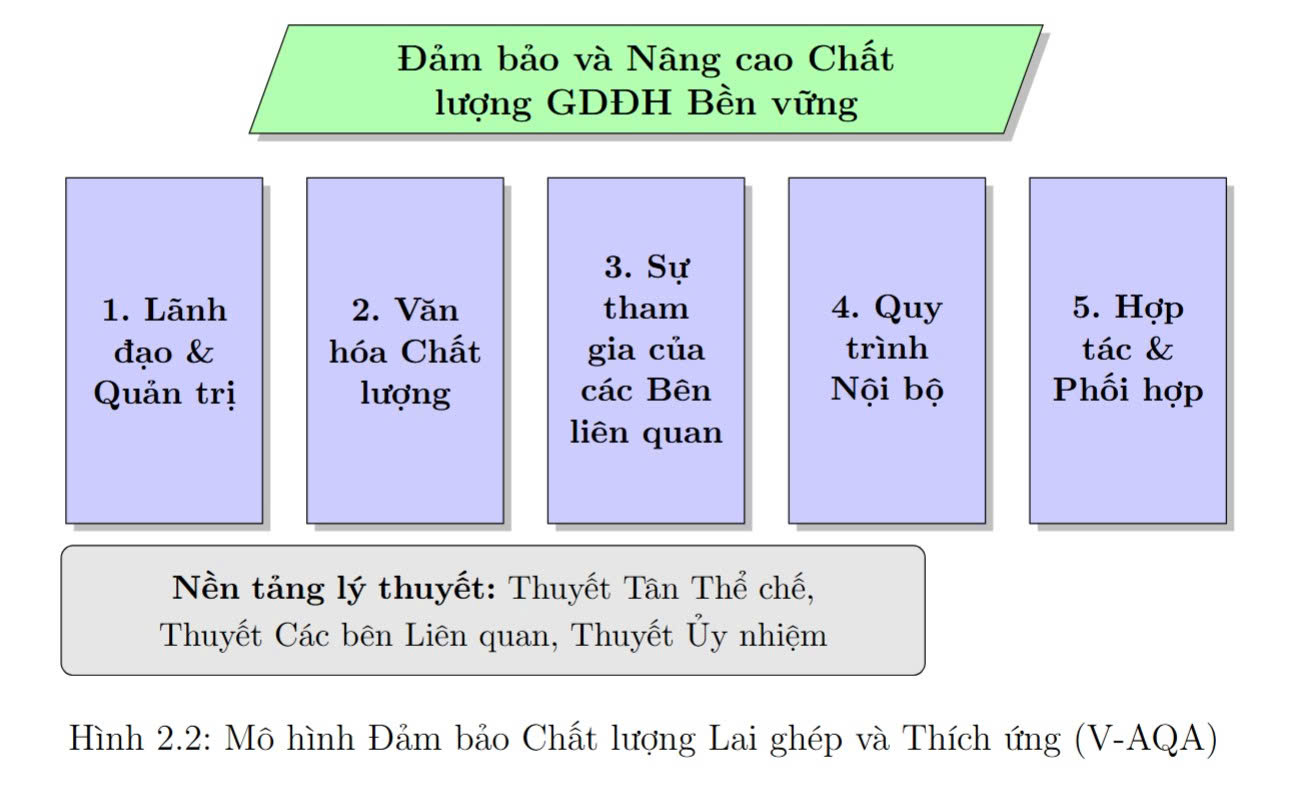
\includegraphics[width=\textwidth]{image/mo_hinh_V-AQA.jpg}
    \caption{混合与适应性质量保障模型 (V-AQA)}
    \label{fig:v-aqa-model-detailed}
\end{figure}

该系统需设计为能自动整合校内多个分散来源的数据,以创建关于质量的360度视图,包括:
\begin{itemize}
    \item \textbf{教学管理系统:} 学生数据、成绩、学习进度、辍学率。
    \item \textbf{人事系统:} 教师的学历、经验、专业发展活动和科研成果数据。
    \item \textbf{科技管理系统:} 研究课题、经费、科学论文数据。
    \item \textbf{在线调查系统:} 来自学生、教师、校友和雇主满意度调查的数据。
    \item \textbf{财务系统:} 用于教学、研究活动的预算分配和使用数据。
\end{itemize}

\paragraph{输出产品:智能报告与仪表盘。}
质量保障管理信息系统的最终目标不是存储数据,而是将数据转化为对各级决策有用的信息。为实现此目标,系统需配备一个\textbf{商业智能}模块,以自动生成可视化的报告和仪表盘,并为不同用户角色进行定制和授权\footcite{uq_kpi_dashboard}。

为更清晰地说明其可行性以及V-AQA模型如何通过数字工具运作,以下是为质量保障管理信息系统上不同角色定制的仪表盘示例。

\begin{table}[h!]
\centering
\caption{校长/校领导班子在质量保障管理信息系统上的关键绩效指标仪表盘示例}
\label{tab:dashboard_hieu_truong}
\begin{tabular}{|p{4.5cm}|p{2.5cm}|p{2.5cm}|p{2cm}|c|}
\hline
\textbf{战略指标(校级)} & \textbf{当前值} & \textbf{与上期比较} & \textbf{年度目标} & \textbf{状态} \\
\hline
12个月后学生就业率 & 92.5\% & $\blacktriangle$ 1.5\% & 95\% & 预警 \\
\hline
国际发表数量(Scopus/ISI) & 350 & $\blacktriangle$ 10\% & 400 & 达标 \\
\hline
雇主满意度 & 4.2/5 & $\blacktriangledown$ 0.1 & 4.5/5 & 未达标 \\
\hline
国际学生比例 & 8\% & $\blacktriangle$ 0.5\% & 10\% & 预警 \\
\hline
科研与技术转让收入 & 500亿 & $\blacktriangle$ 5\% & 600亿 & 预警 \\
\hline
\end{tabular}
\end{table}

\begin{table}[h!]
\centering
\caption{院长在质量保障管理信息系统上的关键绩效指标仪表盘示例}
\label{tab:dashboard_truong_khoa}
\begin{tabular}{|p{5cm}|p{2.5cm}|p{2.5cm}|p{2cm}|c|}
\hline
\textbf{运营指标(信息技术学院)} & \textbf{当前值} & \textbf{与上期比较} & \textbf{年度目标} & \textbf{状态} \\
\hline
按时毕业率 & 85\% & $\longleftrightarrow$ & 90\% & 预警 \\
\hline
学生对培养方案的满意度 & 3.9/5 & $\blacktriangle$ 0.2 & 4.2/5 & 预警 \\
\hline
院级科研课题数量 & 15 & $\blacktriangle$ 2 & 20 & 未达标 \\
\hline
参与培养方案改进的教师比例 & 60\% & $\blacktriangle$ 10\% & 80\% & 未达标 \\
\hline
\end{tabular}
\end{table}

\begin{table}[h!]
\centering
\caption{教师在质量保障管理信息系统上的关键绩效指标仪表盘示例}
\label{tab:dashboard_giang_vien}
\begin{tabular}{|p{5.5cm}|p{2.5cm}|p{3.5cm}|c|}
\hline
\textbf{个人指标(阮文A教师)} & \textbf{本学期} & \textbf{与全院平均比较} & \textbf{备注} \\
\hline
学生对教学的反馈得分 & 4.5/5 & +0.6 & 优秀 \\
\hline
已完成/计划科研时数 & 120/200 小时 & -40 小时 & 需改进 \\
\hline
学生课程通过率 & 95\% & +5\% & 良好 \\
\hline
专业发展活动 & 2门课程 & +1 & 良好 \\
\hline
\end{tabular}
\end{table}
    

部署一个质量保障管理信息系统不仅是一个技术解决方案,更是一场工作方式的改革。它要求领导层的坚定承诺、相应的资源投入,以及一个系统的培训计划,以使全体团队能够有效利用数据的力量。

\subsection{质量保障管理信息系统的风险分析与缓解方案}
\label{subsec:risk_qamis}
尽管带来巨大益处,部署质量保障管理信息系统也面临许多技术和人为风险。

\begin{itemize}
    \item \textbf{风险1:投资和维护成本超出能力。}
    \textit{表现:} 学校没有足够预算来构建、购买许可和维护一个复杂的信息系统。升级、维护和运营人员等隐性成本未被计算在内。
    \textit{缓解策略:}
    \begin{itemize}
        \item \textbf{分阶段实施:} 从最核心的模块开始,如学生数据管理和在线调查。更复杂的模块如商业智能将在证明其有效性后于后续阶段开发。
        \item \textbf{考虑开源解决方案:} 研究并利用开源平台以降低软件许可费用,将预算集中于定制和培训。
    \end{itemize}

    \item \textbf{风险2:数据不同步、不准确(垃圾进,垃圾出)。}
    \textit{表现:} 来自不同部门的数据在格式和可靠性上不一致。如果将“垃圾”数据输入系统,报告和分析将变得毫无意义。
    \textit{缓解策略:}
    \begin{itemize}
        \item \textbf{建立数据治理规定:} 颁布关于数据录入责任、格式标准化以及在集成到统一系统前对各部门数据进行检查、验证流程的明确规定。
        \item \textbf{投资于ETL(提取、转换、加载)过程:} 数据的清洗、转换和集成过程极其重要,需要投入相应的技术资源。
    \end{itemize}
    
    \item \textbf{风险3:来自最终用户的抵制。}
    \textit{表现:} 干部、教师不想使用新系统,因为它复杂、增加了工作量,或者他们感到被“监控”得太紧。
    \textit{缓解策略:}
    \begin{itemize}
        \item \textbf{设计友好的界面并关注用户利益:} 系统设计必须旨在帮助用户减少手工工作(例如:自动生成报告而非手动制作),而不仅仅是服务于管理层。
        \item \textbf{组织持续的培训和支持:} 建立一个支持团队(服务台),并提供直观易懂的指导材料。为特定用户群体组织实践培训。
    \end{itemize}
\end{itemize}

% het goi 7 chuong 4


























	% \chapter{结论与建议}
\label{chap:ket_luan_khuyen_nghi}

%-----------------------------------------------------------------------
% Mục 5.1: Tổng quan và Tóm tắt các Phát hiện Chính
%-----------------------------------------------------------------------

\section{主要研究成果总结与论文定位}
\label{sec:tong_hop_ket_qua}

本章作为总结与结论章节,汇集并凝练了本论文的全部研究成果。在经历了从理论基础分析(第二章)、"解剖"系统现状(第三章)到构建全面改革模型(第四章)的历程后,最后一章将承担三项核心任务:
\begin{enumerate}
    \item \textbf{总结}本论文的主要科学发现与贡献。
    \item \textbf{提出}一套具体可行的政策与行动建议,旨在完善越南高等教育质量保障体系。
    \item \textbf{坦诚地讨论}实施这些建议时面临的挑战、先决条件,同时指出研究的局限性及未来的潜在研究方向。
\end{enumerate}

本章的目标不仅是为研究工作画上句号,更是为政策制定者、教育管理者以及相关方提供一个系统的视角和一份有科学依据的"行动手册",共同致力于可持续地提升越南高等教育质量。

\subsection{现状分析的核心发现总结}
\label{subsec:tom_tat_phat_hien}

第三章详细呈现的对2015-2024年间越南高等教育质量保障体系现状的深入分析,得出了重要结论,勾勒出一幅光明与阴影交织的多维度画面。

\paragraph{论点一:规模上的成就与广泛的合规性。}
不可否认,整个体系在扩大规模和执行质量认证规定方面取得了显著的努力和成就。截至2023-2024学年末,越南高等教育体系已发展到\textbf{243所培养机构,学生规模超过235万}\footcite{thanhnien_quymo_2024}。特别是在质量保障方面,截至2025年初,已有\textbf{208所高等教育机构(占74.8\%)完成了认证周期},并被承认达到国内或国际质量标准\footcite{dantri_kiemdinh_2025}。这些数字显示了在意识和合规行动上的广泛积极转变,为更深层次的质量改进步骤奠定了重要的初步基础。

\paragraph{论点二:"质量悖论"与系统性"恶性循环"的存在。}
然而,在规模和认证比例这些亮眼数字的背后,是一个深刻的"发展悖论"。尽管毕业生在12个月内的就业率相当高,但调查显示,其中只有约\textbf{76\%的人从事与所学专业相符的工作}\footcite{neu_tylevieclam}。这种持续的"不匹配"是一个明确的证据,表明培养质量尚未真正满足劳动力市场的要求。

本论文证明,这一悖论并非偶然,而是具有系统性的"恶性循环"的后果。第三章的分析指出了核心症结,包括:
\begin{itemize}
    \item 一种\textbf{带有合规性和应付色彩的质量文化},这种文化被一种仍然带有浓厚行政色彩和自上而下强加的管理机制所"滋养"\footcite{vjol_reactiveculture}。
    \item 与外部利益相关者,特别是企业界的\textbf{联系松散且缺乏实质性},导致培养方案变得陈旧且缺乏应用性\footcite{worldbank_improvingperformance}。
    \item 最严重的是,一个\textbf{薄弱、碎片化的数据管理系统},被视为体系的"阿喀琉斯之踵",导致改进决策常常缺乏实证依据,未能达到预期效果。
\end{itemize}

清晰地识别这一悖论及其恶性循环,是迫切需要一个整体和系统的解决方案模型而非零散措施的实践基础。这也正是本章后续部分将重点解决的任务。

\subsection{基于V-AQA模型对核心挑战进行系统化梳理}
\label{subsec:he_thong_hoa_thach_thuc}

为获得一个系统的视角并为制定解决方案奠定基础,第三章已分析的挑战将按照V-AQA理论框架的5个要素进行总结。下表\ref{tab:tom_tat_thach_thuc_chuong5}提供了一份综合"诊断书",指出了越南高等教育质量保障体系中问题的"症状"和"根本原因"。

\begin{table}[h!]
\centering
\caption{基于V-AQA模型5要素的系统性挑战总结表}
\label{tab:tom_tat_thach_thuc_chuong5}
\resizebox{\textwidth}{!}{%
\begin{tabular}{|p{3cm}|p{6.5cm}|p{6cm}|}
\hline
\textbf{V-AQA要素} & \textbf{主要挑战/"症状"} & \textbf{根本性系统原因} \\
\hline
\textbf{1. 领导与治理} & 
推动自主的政策与仍带有浓厚合规色彩的管理实践之间的矛盾。领导层将更多精力用于应付行政要求而非质量战略治理\footcite{lypham_aosat_2024}。 & 
"主管部门"机制依然存在,削弱了校董会的实质性自主权\footcite{khuyen_bochuquan_2022}。自主的法律框架不完善且缺乏同步性。 \\
\hline
\textbf{2. 质量文化} & 
"反应型质量文化"占主导,质量保障活动仅为应付认证而季节性进行。教师被动参与,视质量保障为负担\footcite{vjol_reactiveculture}。 & 
自上而下管理模式的后果。缺乏鼓励和表彰实质性改进努力的机制。缺乏关于质量文化的系统性培训项目。 \\
\hline
\textbf{3. 利益相关者的参与} & 
与企业的联系松散,形式化。在培养方案设计中咨询利益相关者(企业、学生)的做法有限,导致"技能差距"\footcite{worldbank_improvingperformance}。 &
"象牙塔思维"的遗留物。缺乏互利共赢的双边合作机制。学生和校友在学术治理中的角色仍然模糊\footcite{pmc_article_9127449}。 \\
\hline
\textbf{4. 内部流程} & 
\begin{itemize}
    \item 培养方案开发流程落后,预期学习成果模糊,打破了"建设性对齐"原则\footcite{ijlter_elo_copy}。
    \item 物质设施和信息通信技术基础设施薄弱\footcite{worldbank_improvingperformance}。
    \item \textbf{"阿喀琉斯之踵":} 数据系统碎片化、不可靠,阻碍了基于证据的治理\footcite{aunsec_redesigningIQA}。
\end{itemize} &
重理论的课程开发思维。投资预算有限,采购流程复杂。在国家和学校层面缺乏一个集成的管理信息系统。 \\
\hline
\textbf{5. 合作与协调} & 
校内"孤岛"状态。各校之间的竞争环境压倒了合作与比对精神。学校、其他学校与社会之间缺乏战略合作模式。 & 
根深蒂固的"本位主义"、"部门主义"思维。缺乏推动实质性经验分享和相互学习的机制与平台。 \\
\hline
\end{tabular}
}
\end{table}

\vspace{0.5cm}

上述综合图景表明,越南质量保障体系的问题并非在于单一的某个方面,而是一系列具有因果关系、相互交织并相互强化的挑战集合。一种被动的质量文化是集权管理模式的后果,而它又反过来使得与企业建立联系或改进内部流程的努力变得更加困难。数据管理的薄弱又使得领导者缺乏战略决策的依据,恶性循环就这样持续下去。

清晰地识别这些系统性挑战及其相互关系,是最重要的科学基础,申明了任何想要成功的改革努力都必须采取一种整体性的方法。不能只专注于培训如何编写预期学习成果而忽略了与企业建立合作机制。同样,如果不能赋予学校实质性的自主权和现代化的管理工具,也不能要求学校进行创新。

基于对这些"瓶颈"的深刻理解,本论文将转到下一部分,申明其在理论和实践方面的贡献,然后提出一套旨在打破已指出的恶性循环的战略性解决方案体系。


% het goi 1 2


\section{本论文的新贡献}
\label{sec:dong_gop_luan_an}

基于实证分析结果,本论文在理论和实践两个层面都做出了具有意义的新贡献。本部分将重点阐明其在理论方面的贡献,申明所构建和验证的分析框架的科学价值与独特性。

\subsection{理论贡献}
\label{subsec:dong_gop_ly_luan}

本论文核心且贯穿始终的理论贡献在于成功构建并论证了一个\textbf{新的综合理论框架——混合与适应性质量保障模型(V-AQA)}。该贡献体现在三个主要方面。

\paragraph{首先,本论文指出了在复杂背景下应用单一理论的局限性。}
如第二章所分析和批判的,当经典的治理理论被独立地应用于像越南这样的转型期国家的高等教育领域时,都暴露了其局限性。
\begin{itemize}
    \item \textbf{新制度主义理论}很好地解释了同形现象以及为获得合法性而产生的合规压力\footcite{MeyerPowell2020},但未能充分解释大学自身的主动性、创新能力和对抗性策略。
    \item \textbf{利益相关者理论}揭示了利益冲突以及为多个群体创造价值的必要性\footcite{Freeman1984},但缺乏分析有形监督机制和塑造利益相关者优先级的权力结构的工具。
    \item \textbf{委托代理理论}为分析问责结构和控制机制提供了一套锐利的工具\footcite{JensenMeckling1976},但有将教育中不仅基于合同,还基于文化和无形规范的复杂关系简单化的风险。
\end{itemize}
通过明确指出这些"盲点",本论文有力地申明了采用一种综合的多理论方法以把握全局的必要性。

\paragraph{其次,本论文成功构建了一个多维度、系统的分析模型。}
V-AQA模型并非机械的拼接,而是将不同理论视角综合并结构化为一个连贯分析框架的努力。该模型的五个要素——(1)领导与治理、(2)质量文化、(3)利益相关者的参与、(4)内部流程,以及(5)合作与协调——是建立在三大基础理论的交汇和互补之上的。
\begin{itemize}
    \item \textit{领导与治理}和\textit{内部流程}要素深受委托代理理论视角的影响。
    \item \textit{质量文化}和\textit{合作与协调}要素通过新制度主义理论得到了清晰的映照。
    \item \textit{利益相关者的参与}要素是利益相关者理论的直接应用。
\end{itemize}
构建这样一个综合模型,提供了一个新的、更全面的分析工具,允许从权力结构、文化规则到技术流程等多个维度来"解剖"质量保障体系的问题。

\paragraph{第三,V-AQA模型在分析转型期国家高等教育体系方面具有特殊的理论价值。}
一个重要的理论贡献在于该模型对特殊背景的适用性。与在欧美国家(拥有悠久的大学自主传统和发达的公民社会)发展的质量保障模型不同,V-AQA模型旨在捕捉像越南这样体系的典型张力:即\textbf{一个强大的、集中的国家管理机制}与来自\textbf{市场和社会利益相关者日益增长的压力}并存\footcite{WB_TransitionalQA}。V-AQA模型,凭借其在问责制与改进之间的"混合"哲学,以及应对变化背景的"适应性"原则,为解释和指导这些处于转型阶段的体系提供了一个更敏锐的理论框架。因此,本论文不仅对越南有价值,也可以在类似的国家背景下得到参考和验证。

总之,通过超越单一理论的局限性并构建一个综合、系统且对背景敏感的分析框架,本论文为丰富高等教育治理和质量保障的理论宝库做出了贡献。

\subsection{实践贡献}
\label{subsec:dong_gop_thuc_tien}

除了理论价值,本论文最重要和最实际的贡献在于其应用能力,即为越南的管理者和政策制定者提供了一个具体的分析框架和行动路线图。

\paragraph{首先,本论文提供了一个系统性诊断工具,用以识别核心"瓶颈"。}
V-AQA模型及第三章的分析为管理者提供了一个系统性的视角来"审视"和"诊断"自己的组织,而不是仅仅描述表面症状。通过从5个相互作用的要素来分析问题,一所大学可以:
\begin{itemize}
    \item 准确确定质量问题的根本原因。例如,学校可以不仅仅得出"学生软技能薄弱"的结论,而是可以追溯到"利益相关者参与"薄弱(没有来自企业的反馈)或"内部流程"薄弱(预期学习成果无法衡量软技能)的根源。
    \item 识别正在抑制自身发展的"恶性循环",例如缺乏数据与决策效率低下之间的循环\footcite{aunsec_redesigningIQA}。
\end{itemize}
这个诊断工具有助于管理者从被动、零散地解决问题,转向主动和系统性的方法。

\paragraph{其次,本论文构建了一份全面且可行的"行动手册"。}
改革努力最大的挑战之一是政策与执行之间的差距\footcite{OECD_PolicyToAction}。本论文通过不仅仅停留在分析,还在第四章中构建了一套解决方案和一个详细的实施路线图,努力缩小这一差距。
\begin{itemize}
    \item \textbf{行动具体化:} 为V-AQA的每个要素提出的解决方案都非常具体,从建立行业咨询委员会、部署质量保障管理信息系统,到为跨学科项目设立资助基金。
    \item \textbf{优先级排序:} 为期7年、分3个阶段的实施路线图(基础与试点、扩展与标准化、优化与传播)提供了一条清晰的路径,帮助学校知道从何处着手以及接下来的步骤。
    \item \textbf{风险管理:} 对每组解决方案的潜在风险进行分析并提出缓解措施,大大增加了模型应用的现实性和成功可能性。
\end{itemize}
这份手册对于各大学的校领导班子、质量保障处负责人以及政策制定者在构建质量改革战略和行动计划的过程中尤其有用。

\paragraph{第三,本论文提供了一个协调的视角,帮助越南各校在一体化背景下定位。}
本论文深入分析了由国家主导的质量保障模型(中国经验)和基于网络、同行合作的模型(东盟大学网络质量保障框架)之间的差异。在此基础上,提出的V-AQA模型如同一条"中间道路",一种有选择的综合,帮助越南大学:
\begin{itemize}
    \item 既能满足一个由国家管理体系的问责要求。
    \item 又能建立内在能力和一种主动的质量文化,以趋近国际标准。
\end{itemize}
这种方法帮助管理者避免了两个极端:要么不适当地机械照搬国际标准,要么封闭、自满于国内的最低规定。

总之,本论文不仅是一部供阅读的著作,更是一套供"使用"的工具。它为"诊断"问题提供了实证实据,为"思考"解决方案提供了理论框架,为"执行"改革提供了行动计划。这正是本论文所追求的最重要的实践贡献。

% het goi 3 4


\section{旨在完善越南高等教育质量保障体系的建议体系}
\label{sec:he_thong_khuyen_nghi}

基于现状分析结果和已确认的科学贡献,本论文提出了一套政策建议和战略行动体系。这些建议并非孤立的解决方案,而是经过精心构建,旨在\textbf{打破第三章已识别的"恶性循环"},并创造一个可持续质量改进的\textbf{"良性循环"}。

该建议体系基于V-AQA模型的核心原则构建:
\begin{itemize}
    \item \textbf{系统性:} 同步作用于模型的全部5个要素,从宏观层面(国家政策)到微观层面(各学校的活动)。
    \item \textbf{可行性:} 建议按优先级划分,并结合越南的实际情况。
    \item \textbf{可衡量性:} 每组行动都提出了具体的关键绩效指标,以便进行跟踪和评估。
\end{itemize}

下表\ref{tab:tong_quan_khuyen_nghi}提供了整个建议体系的概览,按主要对象群体、具体行动、优先级及与V-AQA模型要素的关联进行分类。该表将作为后续详细分析部分的指南。

\begin{longtable}{|p{3.5cm}|p{5.5cm}|p{2cm}|p{3.5cm}|}
\caption{基于V-AQA模型的建议体系概览表}
\label{tab:tong_quan_khuyen_nghi} \\
\hline
\textbf{对象} & \textbf{建议的战略行动} & \textbf{优先级} & \textbf{主要作用的V-AQA要素} \\
\hline
\endfirsthead
\multicolumn{4}{c}%
{{\bfseries \tablename\ \thetable{} -- 续前页}} \\
\hline
\textbf{对象} & \textbf{建议的战略行动} & \textbf{优先级} & \textbf{主要作用的V-AQA要素} \\
\hline
\endhead
\hline \multicolumn{4}{r}{{续下页}} \\
\endfoot
\hline
\endlastfoot

% 第1行:国家管理机构
\textbf{1. 国家管理机构(教育培训部)} & 
1.1. 将角色从微观控制转变为环境创造和宏观调控。 \newline
1.2. 推动基于绩效的拨款机制。 \newline
1.3. 促进一个多样化和竞争性的质量保障生态系统,承认国际质量认证组织。 \newline
1.4. 战略性投资建设集成的国家高等教育数据系统。 & 
短期 (1.1, 1.4) \newline 中期 (1.2, 1.3) & 
1. 领导与治理 \newline
5. 合作与协调 \\
\hline

% 第2行:高等教育机构
\textbf{2. 高等教育机构} & 
2.1. 实质性地制定并执行校级质量战略。 \newline
2.2. 发起从基层建设质量文化的运动。 \newline
2.3. 建立并机制化行业咨询委员会的运作。 \newline
2.4. 按照成果导向教育实现培养方案开发流程现代化并多样化评估方法。 \newline
2.5. 投资建设质量保障管理信息系统。 \newline
2.6. 主动参与标杆比对和同行评审网络。 & 
短期 (2.1, 2.2) \newline 中期 (2.3, 2.4, 2.5) \newline 长期 (2.6) & 
同步作用于V-AQA模型的全部5个要素。 \\
\hline

% 第3行:质量认证中心
\textbf{3. 质量认证中心} & 
3.1. 提升认证员队伍的专业能力和职业素养。 \newline
3.2. 为不同类型的学校开发专门的评估标准或指南。 \newline
3.3. 加强结果和综合分析报告的公开透明化。 & 
中期 & 
4. 内部流程 \newline
5. 合作与协调 \\
\hline

% 第4行:各协会
\textbf{4. 企业与行业协会} & 
4.1. 主导构建"职业能力框架"。 \newline
4.2. 主动参与行业咨询委员会及培养方案评估活动。 & 
中期 & 
3. 利益相关者的参与 \\
\hline

\end{longtable}

\vspace{0.5cm}

如上表所示,各项建议并非仅集中于单一主体,而是要求从国家管理机构、各大学到认证组织和企业界等整个教育生态系统的共同努力和同步行动。每组行动都旨在解决已分析的相应"瓶颈",最终目标是在质量的思维和行动上实现根本性转变。

本章的后续部分将深入分析和论证每一组建议,包括其科学依据、需要开展的具体行动以及配套的关键绩效指标。

\subsection{对国家管理机构的建议}
\label{subsec:khuyen_nghi_qlnn_detailed}

作为体系的"总建筑师",国家管理机构,直接是教育培训部,在为质量改革创造有利的制度环境方面扮演着决定性角色。以下建议侧重于将国家角色从直接控制转变为环境创造和宏观调控,这一趋势已在许多先进教育体系中被证明有效\footcite{OECD_PolicyToAction}。

\subsubsection{建议1.1:将角色从"微观控制者"转变为"环境创造者和宏观调控者"}

\paragraph{论据:}
第三章的分析指出了一个核心矛盾:虽然宏观政策朝向自主,但具体的管理机制仍然带有浓厚的行政色彩,催生了"合规文化",并削弱了学校实质性改进的动力\footcite{pham2021governance}。教育培训部颁布的包含过多流程性、程序性标准的评估标准(例如,根据第12/2017号通知的25项标准\footcite{tt12_2017_bgddt}),无意中引导了各学校专注于应付性地完善档案,而非进行战略性改进。

为使\textbf{2018年修订的《高等教育法》}\footcite{luatvn_gddh_2018}精神真正落到实处,国家管理机构需要转变其角色。国家不应是"手把手指导者",而应是建立公平"游戏规则"者,监督最低标准的遵守情况,最重要的是,推动一个透明的环境,以便社会能够发挥其监督作用。这是从委托代理理论(委托人严密监督代理人)向更现代的治理模式的转变,即国家本着新制度主义精神,创造一个健康的"制度场域"。

\paragraph{具体行动:}
\begin{enumerate}
    \item \textbf{改革质量认证标准:} 研究修订教育机构和培养项目的质量认证标准,使其更精简,侧重于产出和核心质量保障条件(例如:师资能力、基础设施、有效治理),减少带有浓厚行政流程、程序色彩的标准。新标准需要有"开放空间",让各校可以根据自身使命和独特战略,以不同方式证明其质量。
    
    \item \textbf{加强"认证认证机构"的角色:} 教育培训部需要专注于建立严格监督各质量认证中心活动运作的标准和流程,确保这些组织的独立性、专业性和道德性。赋予认证中心更大的权力和更高的问责要求,逐步减少教育部对具体评估活动的直接干预。
    
    \item \textbf{建立国家高等教育质量信息门户:} 建立一个单一的电子信息门户,在此\textbf{完全}公开所有高等教育机构的自评报告、外部评估报告以及主要质量指标(例如:就业率、规模、师资队伍)。这种透明度是最有效的社会监督工具,能创造健康的竞争压力,并迫使各校对其质量真正负责。
\end{enumerate}

\paragraph{关键绩效指标:}
\begin{itemize}
    \item 新标准体系中侧重于产出的标准与侧重于投入/流程的标准的比例。
    \item 各大学和认证中心对新政策的清晰度和支持性的满意度。
    \item 国家质量信息门户的数据访问和利用次数。
\end{itemize}

\subsubsection{建议1.2:推动基于绩效的拨款机制}

\paragraph{论据:}
单纯的行政压力通常只能带来合规。要创造实质性的改进动力,需要有财政激励工具。已在许多经合组织国家成功应用的基于绩效的拨款机制,是一个强大的政策工具,能将各校的重点从维持运作转向追求卓越\footcite{oecd_pbf_2021}。通过将部分预算与产出结果挂钩,国家将发出一个明确的信息:"质量将得到奖赏"。这将促使各校领导层更具战略性地思考如何改善核心质量指标。

\paragraph{具体行动:}
\begin{enumerate}
    \item \textbf{构建国家基于绩效的拨款指标体系:} 教育培训部主导,与专家、各大学及相关方协调,构建一套清晰、透明且可衡量的关键绩效指标体系,作为预算分配的依据。该指标体系可包括以下几组:
        \begin{itemize}
            \item \textit{培养质量:} 毕业生12个月内从事对口工作的比例(数据来自高等教育管理信息系统与社会保险系统联动),学生满意度。
            \item \textit{研究能力:} 每位教师在权威期刊(Scopus/WoS)上的国际发表数量,来自科技活动和知识转移的收入。
            \item \textit{国际化水平:} 国际学生和教师比例,由权威国际组织认证的项目数量。
        \end{itemize}
    \item \textbf{按路线图进行试点:} 开始在已实现自主的公立大学群体中试点实施基于绩效的拨款机制。在初期阶段,可以根据关键绩效指标的达成结果分配一部分预算(例如:总经常性支出的10-20%)。
    \item \textbf{评估与调整:} 每2-3年周期后,需要有一份独立的影��评估报告,分析基于绩效的拨款机制的积极和消极影响(如有),从而在考虑推广前,对关键绩效指标体系和分配方式进行适当调整。
\end{enumerate}

\paragraph{关键绩效指标:}
\begin{itemize}
    \item 按基于绩效的拨款机制分配的高等教育预算百分比。
    \item 试点院校群体的关键绩效指标平均改善程度与非试点院校群体的比较。
    \item 各大学对基于绩效的拨款机制的共识度和支持度。
\end{itemize}


% het goi 5 6


\subsubsection{建议1.3:促进一个多样化和竞争性的质量保障生态系统}

\paragraph{论据:}
一个质量保障体系只有在评估主体多样化且他们之间存在良性竞争时,才能真正有效。过度依赖少数几家仍受教育培训部管理的国内认证中心,可能导致缺乏客观性且不鼓励创新\footcite{giaoducnet_kdcl_list_2023}。相反,开放并承认有信誉的国际认证组织将带来诸多好处:
\begin{itemize}
    \item \textbf{增强客观性与国际接轨:} 国际认证组织按全球标准运作,帮助越南大学客观地看待自身质量,并加速国际化进程。实际上,已有\textbf{11所越南大学获得了像德国工商管理认证基金会、英国质量保障署、法国高等教育与研究评估高等委员会等国外权威组织的认证},这表明顶尖大学确有接轨的需求和能力\footcite{thuvienphapluat_11truong_quocte}。
    \item \textbf{创造积极的竞争压力:} 国际组织的存在将产生压力,迫使国内认证中心不断提升其专业能力和服务质量以求竞争。
    \item \textbf{推动按专业领域的认证:} 许多国际组织专门从事特定领域的认证(例如:工程领域的ABET,商科领域的AACSB)。参与专业认证将有助于各院系实质性地提升培养质量,并使其与各行业的要求相符。
\end{itemize}

\paragraph{具体行动:}
\begin{enumerate}
    \item \textbf{颁布承认国际认证结果的规定:} 建立并颁布一个通畅透明的法律走廊,用于承认有信誉的国际组织的认证结果,特别是那些全球网络如\textbf{国际高等教育质量保障机构网络}或区域网络如\textbf{亚太质量网络}的成员组织。
    \item \textbf{鼓励专业认证:} 为优先领域(技术、工程、经济、健康)的培养项目参与并获得世界公认的专业组织认证提供具体鼓励政策(例如:资助部分经费,在评优项目中加分)。
    \item \textbf{推动行业协会的角色:} 创造机制,让国内的行业协会(例如:建筑工程师协会、越南会计与审计协会)参与构建职业能力标准,并逐步参与相关培养项目的评估和承认。
\end{enumerate}

\paragraph{关键绩效指标:}
\begin{itemize}
    \item 获得有信誉的国际组织认证的培养项目数量。
    \item 成为国际网络(国际高等教育质量保障机构网络、亚太质量网络)成员的国内认证中心比例。
    \item 由行业协会颁布并被各校用作参考的职业能力标准数量。
\end{itemize}

\subsubsection{建议1.4:战略性投资建设集成的国家高等教育数据系统}

\paragraph{论据:}
正如多次分析和强调的,数据的薄弱和碎片化是越南高等教育治理体系的"阿喀琉斯之踵"\footcite{aunsec_redesigningIQA}。缺乏同步和可靠的数据,所有宏观管理努力,从政策规划、按绩效拨款到人力需求预测,都变得缺乏科学依据。颁布关于教育行业统计报告制度的\textbf{第25/2024号通知}是朝着正确方向迈出的一步,但需要一个足够强大的技术系统来实现\footcite{luatvietnam_tt25_2024}。

因此,投资建设一个国家高等教育管理信息系统不应被视为一项开支,而应是对\textbf{治理基础设施的一项战略投资},有可能为整个体系带来巨大的效率和透明度回报。

\paragraph{具体行动:}
\begin{enumerate}
    \item \textbf{成立国家高等教育管理信息系统指导委员会:} 教育培训部应主导,与相关部委(计划与投资部、财政部、信息与通信部、越南社会保险)协调,制定一个总体方案并为此项目分配国家资源。
    
    \item \textbf{设计现代化的系统架构:} 国家高等教育管理信息系统需被设计为一个国家\textbf{数据仓库},能够按照一个共同标准整合来自各校信息系统的数据。核心功能包括:收集、清洗、存储、分析和数据可视化。
    
    \item \textbf{部署突破性构件——与社会保险数据联通:} 这是一个旨在解决衡量产出质量难题的革命性方案。建立机制(有严格的个人信息保密规定),将毕业生数据(根据个人身份识别码)与越南社会保险的数据库进行比对。这将提供关于以下方面的\textbf{客观、准确和实时更新}的图景:
        \begin{itemize}
            \item 学生的实际就业率。
            \item 按学校、专业的平均收入水平。
            \item 获得第一份工作的平均时间。
            \item 职业流动和从事与专业不符工作的比例。
        \end{itemize}
    这些数据将是基于绩效的拨款机制最重要的输入,并帮助社会对每个培养项目的真实"价值"有一个透明的了解。
    
    \item \textbf{建立开放数据(Open Data)利用政策:} 在匿名化处理后,一部分高等教育管理信息系统的数据应以开放数据的形式公布,以便研究人员、独立组织和社会可以利用,进行深入分析,有助于推动一个透明和基于证据的治理。
\end{enumerate}

\paragraph{关键绩效指标:}
\begin{itemize}
    \item 已连接并与国家高等教育管理信息系统同步数据的高等教育机构百分比。
    \item 汇总和公布全行业统计报告的平均时间(从每年减少到每季度/每月)。
    \item 基于国家高等教育管理信息系统数据构建的政策分析报告数量。
\end{itemize}

\subsection{对高等教育机构的建议}
\label{subsec:khuyen_nghi_csgddh_detailed}

虽然国家的宏观政策创造了环境和法律走廊,但质量的实质性转变必须来自每所大学自身的内部努力。以下建议按照V-AQA模型的五个要素构建,旨在为教育管理者提供一个具体的行动框架,以从内部引领变革。

\subsubsection{建议2.1:重构领导与治理——从"控制者"转变为"环境创造者"}

\paragraph{论据:}
首要需要解开的症结是领导团队的角色。如第三章所分析,当领导者陷入行政管理和应付合规要求时,他们将没有精力和远见来执行其战略角色\footcite{lypham_aosat_2024}。为打破此恶性循环,高层领导(校董会、校领导班子)的角色需要重新定位。他们不是直接从事质量工作的人,而是为质量能够在各级生根发芽和发展创造一个制度、文化和资源环境的人,这符合"创业型大学"的精神\footcite{clark_1998}。

\paragraph{具体行动:}
\begin{enumerate}
    \item \textbf{制定并承诺执行校级质量战略:} 领导层必须主导制定一份正式的五年期\textbf{质量战略},并将其融入学校的总体发展战略中。该文件不应束之高阁,而应是所有行动的指南,其中必须明确定义:质量愿景、优先目标、具体的关键绩效指标以及相应的资源分配计划。
    \item \textbf{强力分权并辅以问责制:} 在学术事务(改进培养方案、创新教学方法)上给予院/系更实质性的自主权。同时,建立一套清晰的关键绩效指标体系来衡量各单位的绩效。领导层将通过质量保障管理信息系统执行战略监督角色,而不是对日常运作进行微观干预。
    \item \textbf{投资于中层管理团队的治理能力:} 为院/系主任、副主任、处室负责人组织关于现代大学治理、变革管理和数据驱动决策的强制性培训项目。这是对"继任团队"的投资,以确保改革的可持续性。
\end{enumerate}

\paragraph{关键绩效指标:}
\begin{itemize}
    \item 每年在质量战略中设定的目标的完成率。
    \item 院/系领导对所获自主权程度的满意度调查得分。
    \item 100%的中层管理干部在两年内完成现代治理培训课程。
\end{itemize}

\subsubsection{建议2.2:塑造质量文化——从"应付"到"主动"}

\paragraph{论据:}
质量文化是无形资产,但决定了所有质量保障体系的成败。一个拥有最佳流程的体系,如果由抱着应付、被动心态的人来运作,也终将失败\footcite{iosr_passiveparticipation}。因此,从"合规文化"向"改进文化"的转型是一项战略性任务,需要采取既作用于组织中每个成员的认知又作用于其行动的解决方案\footcite{HarveyStensaker2008}。

\paragraph{具体行动:}
\begin{enumerate}
    \item \textbf{发起宣传和意识提升运动:} 组织如年度"质量周"、 "教学创新创举"竞赛、关于质量问题的开放论坛等活动。目标是让所有成员明白,质量不仅是质量保障处的责任。
    \item \textbf{建立表彰和奖励改进创举的体系:} 设立年度奖项("教学创新年度教师奖"、"高效质量保障模式院系奖")。更重要的是,将对质量改进的贡献标准纳入干部、教师的评估、评级和晋升流程中。
    \item \textbf{为"质量改进小组"赋能:} 在系级成立由自愿教师组成的小组(质量圈),任务是定期讨论并提出改进教学质量的方案。学校需要提供小额预算("创举支持基金"),以便这些小组可以试验新想法。
\end{enumerate}

\paragraph{关键绩效指标:}
\begin{itemize}
    \item 全校范围内关于质量文化认知的定期调查得分(逐年提高)。
    \item 每年提出并获资助实施的改进创举数量。
    \item 自愿参与质量改进活动的教职工比例。
\end{itemize}


% het 7 8 chuong 5


\subsubsection{建议2.3:将利益相关者从"咨询对象"转变为"战略伙伴"}

\paragraph{论据:}
"技能差距"\footcite{britishcouncil_skills_gap_2021}最深层的原因之一,是在学术流程中缺乏来自利益相关者,特别是雇主和校友的实质性声音。咨询活动(如果有的话)通常仅停留在形式化和被动的层面,如单向咨询或影响甚微的调查\footcite{vnujs_er_3848}。为打破"象牙塔壁垒",学校需要主动创造机制,使利益相关者成为共同创造价值的伙伴,这符合阿恩斯坦(1969)"参与阶梯"最高阶梯的精神\footcite{Arnstein1969}。

\paragraph{具体行动:}
\begin{enumerate}
    \item \textbf{将行业咨询委员会机制化并赋权:}
    学校需要为院系/专业层面成立行业咨询委员会并颁布正式的运作章程,而不是依赖个人关系。行业咨询委员会的角色不仅是咨询,还必须被赋予具体权力:
        \begin{itemize}
            \item \textbf{强制性审定}培养方案的预期学习成果。
            \item \textbf{定期参与}(每年至少1-2次)培养方案的审查和更新会议。
            \item \textbf{共同指导}和评估学生的毕业设计项目。
        \end{itemize}
    该模型是东盟大学网络质量保障\footcite{aunqa_guidelines_v4}和ABET\footcite{abet_criteria}等国际认证标准的核心要求,将创造一个可持续的对话与合作渠道,确保培养方案始终与实践相符。

    \item \textbf{提升学生和校友的角色:}
        \begin{itemize}
            \item \textbf{在学术委员会中为学生赋权:} 让(通过民主选举产生的)学生代表成为院/校级科学与培养委员会中拥有\textbf{投票权}的正式成员。
            \item \textbf{建立主动的"校友大使"网络:} 建立一个由事业有成且热心的校友组成的体系,其作用是定期提供关于培养方案契合度的反馈,并参与为低年级学生提供职业导向活动。
        \end{itemize}
\end{enumerate}

\paragraph{关键绩效指标:}
\begin{itemize}
    \item 来自行业咨询委员会的建议被记录并整合到培养方案改进计划中的百分比。
    \item 有学生代表参与并投票的学术决策数量。
    \item 企业对毕业生工作胜任度的满意度得分(逐年提高)。
\end{itemize}

\subsubsection{建议2.6:通过合作与比对打破"筒仓思维"}

\paragraph{论据:}
在一个孤立的环境中,质量无法得到可持续的改进。各处、室、院系之间的"孤岛"状态以及各校之间不健康的竞争,削弱了整个体系的协同力量和学习能力。要成为一个真正的"学习型组织"\footcite{Senge2006},各校需要主动创造在内部、校际和国际三个层面上的合作机制。

\paragraph{具体行动:}
\begin{enumerate}
    \item \textbf{促进内部合作:} 设立一个\textbf{专门资助跨单位质量改进项目的基金}。优先为有多个院、处、室参与的项目提供经费(例如:"提升软技能"项目需要学生工作处、各专业院系和质量保障处的协调)。
    
    \item \textbf{建立校际标杆比对网络:} 同一专业领域或地区的学校需要主动成立\textbf{质量标杆比对俱乐部}\footcite{jackson_lund_2000}。这些俱乐部可以:
        \begin{itemize}
            \item 通过一个中立的第三方,统一并分享(已匿名的)关于质量指标的数据集。
            \item 组织定期的同行评审活动和"最佳实践"分享研讨会。
        \end{itemize}
    该机制将把竞争转化为学习的动力,帮助各校客观地认识自己的优势和劣势。

    \item \textbf{战略性地利用国际合作活动:} 参与国际认证不应仅停留在获得证书的目标上。学校需要将一个\textbf{"认证后"流程制度化},其中质量保障处必须制定一个具体的行动计划来落实专家组的建议,跟踪进度并向校领导班子报告。
\end{enumerate}

\paragraph{关键绩效指标:}
\begin{itemize}
    \item 每年成功实施的跨院系/处室改进项目数量。
    \item 组织的标杆比对活动数量以及基于比对结果实施的改进措施数量。
    \item 按计划完成的国际认证建议的百分比。
\end{itemize}

\subsubsection{建议2.4与2.5:流程现代化与数据基础设施建设}

\paragraph{论据:}
第三章的分析已指出,内部流程,特别是课程开发流程和数据管理系统,正是越南质量保障体系的"阿喀琉斯之踵"。一个落后、脱节的培养方案开发流程将产生不合格的产品\footcite{ijlter_elo_copy}。同样,一个薄弱的数据系统将瘫痪基于证据的决策能力,使所有改进努力都变得盲目且低效\footcite{aunsec_redesigningIQA}。因此,实现这些流程的现代化并构建一个坚实的技术基础设施是强制性任务,是整个V-AQA模型能够运作的"硬件"基础。

\paragraph{具体行动1:按照成果导向教育理念标准化培养方案开发流程。}
V-AQA模型建议各大学全面转向基于\textbf{成果导向教育}理念的培养方案开发方法。这种方法有助于确保培养目标、教学活动和评估方法之间的紧密联系("建设性对齐"原则\footcite{biggs_constructive_alignment})。为避免形式化应用,该流程必须包括五个紧密相连的步骤:
\begin{enumerate}
    \item \textbf{利益相关者需求分析:} 始于收集和分析来自劳动力市场、行业专家和校友的要求。
    \item \textbf{预期学习成果的制定与审定:} 专业院系制定清晰、可衡量的预期学习成果,且必须由\textbf{行业咨询委员会强制性审定}。
    \item \textbf{设计课程地图:} 构建矩阵,清晰展示每门课程如何为实现预期学习成果做出贡献。
    \item \textbf{审定与批准:} 完整的培养方案必须由科学与培养委员会(包括外部专家)批准。
    \item \textbf{定期审查与改进:} 建立正式的培养方案审查周期(2-3年一次),基于利益相关者的反馈和实际学习成果。
\end{enumerate}

\paragraph{具体行动2:构建集成的质量保障管理信息系统。}
为打破数据恶性循环,V-AQA模型提出了一个基础性的技术解决方案:构建一个集成的\textbf{质量保障管理信息系统}。这是学校的"神经系统",任务是将来自各分散来源(教学、人事、调查、财务、科研)的数据整合到一个单一的\textbf{数据仓库}中。
质量保障管理信息系统的最终目标是将原始数据转化为对各级决策有用的信息。为实现此目标,系统需配备一个\textbf{商业智能}模块,以自动生成可视化的报告和仪表盘,并为不同用户角色进行定制和授权\footcite{educause_bi_2022}。例如:
\begin{itemize}
    \item \textbf{校领导班子仪表盘:} 显示校级战略关键绩效指标,如就业率、国际发表数量、雇主满意度(如表\ref{tab:dashboard_hieu_truong})。
    \item \textbf{院长仪表盘:} 显示院级运营关键绩效指标,如按时毕业率、学生对培养方案的满意度、院级科研课题数量(如表\ref{tab:dashboard_truong_khoa})。
    \item \textbf{教师仪表盘:} 提供关于教学活动的反馈、所负责班级学生的学习成果以及个人任务的执行进度(如表\ref{tab:dashboard_giang_vien})。
\end{itemize}
部署一个质量保障管理信息系统不仅是一个技术解决方案,更是一场工作方式的改革,需要领导层的坚定承诺和对用户的系统培训计划。

\paragraph{关键绩效指标:}
\begin{itemize}
    \item 按照五步成果导向教育流程构建和审查的培养方案百分比。
    \item (院级及以上)发布的、引用或基于质量保障管理信息系统数据的管理决策比例。
    \item 各级管理人员和教师对质量保障管理信息系统的实用性和便利性的满意度。
\end{itemize}


% het goi 9 10 chuong 5



\section{讨论:挑战、条件与前景}
\label{sec:ban_luan_trien_vong}

提出一个全面的改革模型是必要的,但在实践中成功实施该模型则是一个更大的挑战。本部分将坦诚地讨论应用V-AQA模型时最大的困难和障碍,其中,大学自主问题被视为基础性且具有决定性的因素。

\subsection{大学自主:一个有效质量保障体系的先决条件}
\label{subsec:banluan_tuchu}

纵观本论文的分析和建议,大学自主的角色始终被强调为一个基础性因素。可以肯定地说,\textbf{大学自主并非一个选项,而是V-AQA模型及质量改进方案能够成功和可持续实施的先决条件}。一个质量保障体系只有在大学被赋予权力和创新空间的环境中,才能最大限度地发挥其效用\footcite{eua_autonomy_qa}。

这种关系是辩证的。如果没有在学术、人事组织和财务方面的实质性自主权,领导者和教师将没有足够的动力和工具来按照V-AQA模型进行改革。反之,成功实施V-AQA模型,凭借其数据的透明度和明确的问责制,正是一所大学证明自己值得被赋予更大自主权的最好方式。

因此,实施V-AQA不能脱离执行\textbf{2018年修订的《高等教育法》}的路线图\footcite{luatvn_gddh_2018}。该模型的成功程度将直接取决于学校被赋予的自主程度。下面的矩阵图(图\ref{fig:matrix_vqa_autonomy})分析了V-AQA各要素在三种不同自主情景下的运作情况。

\begin{figure}[h!]
    \centering
    \caption{V-AQA模型按大学自主程度的运作矩阵}
    \label{fig:matrix_vqa_autonomy}
    \resizebox{\textwidth}{!}{%
    \begin{tabular}{|p{3cm}|p{4.5cm}|p{4.5cm}|p{4.5cm}|}
    \hline
    \textbf{V-AQA要素} & \textbf{低自主情景} \newline \textit{(合规环境)} & \textbf{中等自主情景} \newline \textit{(转型环境)} & \textbf{高自主情景} \newline \textit{(改进环境)} \\
    \hline
    \textbf{1. 领导与治理} & 领导主要执行行政命令,专注于满足主管部门的报告要求。 & 开始有战略决策的空间,但仍受行政规定约束。领导角色具有"混合"性质。 & 领导真正扮演战略创造者的角色。校董会在导向和监督方面拥有实质性权力。 \\
    \hline
    \textbf{2. 质量文化} & "反应型"和应付式文化。质量保障被视为负担,仅在有认证要求时才进行。 & 合规文化与改进文化之间存在拉锯。试点单位的"速赢"对于创造动力至关重要。 & 改进文化深入所有活动。质量是每个成员的内在责任。创新精神受到鼓励。 \\
    \hline
    \textbf{3. 利益相关者的参与} & 联系是形式化的,主要为完善证明档案。行业咨询委员会(如有)仅具装饰性。 & 行业咨询委员会开始被更系统地建立。在咨询中开始倾听学生的声音。 & 利益相关者(企业、学生、校友)成为"战略伙伴",共同创造课程和学校的价值。 \\
    \hline
    \textbf{4. 内部流程} & 流程僵化,按国家统一规定标准化。质量保障管理信息系统仅是用于导出报告的工具。 & 少数先锋院/系获准试点新流程(成果导向教育、基于项目的学习)。质量保障管理信息系统开始用于内部分析。 & 流程灵活,具有高度适应性。质量保障管理信息系统成为"神经系统",是各级基于证据决策不可或缺的工具。 \\
    \hline
    \textbf{5. 合作与协调} & 合作受限,通常仅按上级指示进行。"暗中竞争"和"保护领地"的思维普遍存在。 & 与企业和校际的合作活动开始在某些领域被主动推动,但尚未成体系。 & 学校主动领导标杆比对网络,与企业和国际伙伴进行战略性、可持续的研发合作。 \\
    \hline
    \end{tabular}
    }
\end{figure}

该矩阵显示,推动大学自主不仅是一项孤立的政策,更是一个能够"解锁"V-AQA模型全部五个要素潜力的杠杆。缺少这个杠杆,再好的改革建议也难以发挥全部作用。因此,完善法律走廊并扫除障碍,使各校能够充分且负责任地行使自主权,是国家在下一阶段的核心任务,为实质性地提升高等教育质量创造前提。

\subsection{风险分析与成功条件}
\label{subsec:risk_analysis_conditions}

实施像V-AQA这样全面和系统性的改革模型,必然会面临诸多风险和挑战。识别、分析并制定应对这些风险的策略,是确保改革过程成功的先决条件\footcite{kerzner_pm_2017}。本部分将重点关注三大风险群:(1)资源风险,(2)人与文化风险,以及(3)政策环境风险。

\subsubsection{风险分析与应对矩阵}
为获得一个全面和系统的视角,矩阵\ref{tab:risk_matrix}将总结主要风险,评估其影响程度和发生可能性,并提出相应的缓解措施。

% --- 已修改代码开始 ---
\begin{filecontents*}{risk_matrix.tex}
\begin{longtable}{|p{2.8cm}|>{\raggedright\arraybackslash}X|p{1.7cm}|p{1.7cm}|>{\raggedright\arraybackslash}X|}
\caption{实施V-AQA模型的风险分析与应对矩阵}
\label{tab:risk_matrix}\\
\hline
\textbf{风险类别} & \textbf{具体风险描述} & \textbf{发生可能性} & \textbf{影响程度} & \textbf{缓解/应对措施} \\
\hline
\endfirsthead
\multicolumn{5}{c}%
{{\bfseries \tablename\ \thetable{} -- 续前页}} \\
\hline
\textbf{风险类别} & \textbf{具体风险描述} & \textbf{发生可能性} & \textbf{影响程度} & \textbf{缓解/应对措施} \\
\hline
\endhead
\hline \multicolumn{5}{r}{{\textit{续下页}}} \\
\endfoot
\hline
\endlastfoot

% 风险1:资源
\textbf{1. 资源(财务、物质设施)} & 
缺乏预算投资于战略性项目,如构建质量保障管理信息系统、升级物质设施以及培训、奖励项目。 & 
高 & 
高 & 
- 制定详细的财务计划,分阶段实施。 \newline
- 多样化收入来源,推动公私合作伙伴关系以动员企业资源。 \newline
- 优先考虑开源技术解决方案以降低许可成本。 \\
\hline

% 风险2:人与文化
\textbf{2. 人与文化} & 
\begin{itemize}
    \item 干部、教师队伍的惰性、不愿改变的心态和怀疑态度。
    \item 感到利益受损的中层管理(暗中或公开)的抵制。
    \item 缺乏具备数据分析和现代治理能力的人力资源。
\end{itemize} & 
非常高 & 
非常高 & 
- 最高层领导的坚定政治承诺和模范作用。 \newline
- 持续、透明地宣传改革的益处。专注于创造"速赢"\footcite{kotter_1996}。 \newline
- 组织关于变革管理和新技能的强制性培训课程。 \newline
- 建立对创新努力的实质性表彰、奖励政策。 \\
\hline

% 风险3:政策
\textbf{3. 宏观政策环境} & 
自主政策与其他规定(财务、人事、公共投资)之间缺乏同步性,限制了各校的行动空间和能力。 & 
中 & 
非常高 & 
- 各大学需通过协会(例如:越南大学与学院协会)主动向教育培训部和政府提出基于证据的政策建议。 \newline
- 教育培训部主导,与相关部委协调,审查并移除不再适宜的政策障碍。 \\
\hline

\end{longtable}
\end{filecontents*}

% --- 开始:风险分析与应对矩阵 ---
\renewcommand{\arraystretch}{1.3} % 增加行距以便阅读

\begin{longtable}{|p{2.5cm}|p{5cm}|p{1.5cm}|p{1.5cm}|p{5cm}|}
\caption{实施V-AQA模型的风险分析与应对矩阵}
\label{tab:risk_matrix}\\
\hline
\textbf{风险类别} & \textbf{具体风险描述} & \textbf{可能性} & \textbf{影响程度} & \textbf{缓解/应对措施} \\
\hline
\endfirsthead
\multicolumn{5}{l}{\textit{(续表 \ref{tab:risk_matrix})}}\\\hline
\textbf{风险类别} & \textbf{具体风险描述} & \textbf{可能性} & \textbf{影响程度} & \textbf{缓解/应对措施} \\
\hline
\endhead
\hline \multicolumn{5}{r}{\textit{续下页}}\\
\endfoot
\hline
\endlastfoot

\textbf{1. 资源} &
缺乏用于质量保障管理信息系统(QA-MIS)、升级设施、培训和奖励的预算。 &
高 &
高 &
\begin{itemize}
  \item 分阶段实施 (phased implementation)。
  \item 收入来源多样化,推动公私合作(PPP)。
  \item 优先采用开源技术。
\end{itemize} \\
\hline

\textbf{2. 人员与文化} &
\begin{itemize}
  \item 干部的惰性、变革抵触和怀疑心态。
  \item 来自中层管理的抵制。
  \item 缺乏数据分析和现代治理专家。
\end{itemize} &
非常高 &
非常高 &
\begin{itemize}
  \item 高层领导的承诺和示范作用。
  \item 透明沟通,创造“短期胜利”。
  \item 关于变革管理的强制性培训。
  \item 对创新给予实质性奖励。
\end{itemize} \\
\hline

\textbf{3. 政策环境} &
自主权与财务、人事、公共投资等规定之间缺乏同步性。 &
中 &
非常高 &
\begin{itemize}
  \item 学校通过协会主动提出政策建议。
  \item 教育培训部与各部委协调,审查并消除政策障碍。
\end{itemize} \\
\hline

\end{longtable}
% --- 结束:风险分析与应对矩阵 ---
    

\subsubsection{成功条件的深入分析}

从上述风险矩阵中,可以得出对V-AQA模型改革过程成功至关重要的三个先决条件。

\paragraph{条件一:来自最高层的强有力且持久的政治承诺。}
这是最重要的因素。转型过程不可避免地会遇到困难、冲突和短期内的效率下降。如果没有来自校董会和校领导班子足够强大、一致和坚韧的承诺,所有改革努力都将轻易地在遇到初步压力时偏离方向或半途而废。这种承诺必须通过具体行动来体现,从率先垂范、分配相应资源到保护敢于创新的人。

\paragraph{条件二:构建一个系统的变革管理战略。}
不能凭主观意愿强加变革。学校需要有一个有效的内部沟通战略,清晰地解释"为什么要变革?","变革将为每个个人和整个组织带来什么好处?"。建立一个包括各单位有威望人士的"变革领导联盟",并专注于创造"速赢"以建立信任和动力,是已被证明有效的战略步骤\footcite{kotter_1996}。

\paragraph{条件三:对技术基础设施和人的能力进行相应投资。}
质量保障管理信息系统是模型的"硬脊梁",而团队的数据分析和现代治理能力是"软脊梁"。这两个因素必须得到并行和相应的投资。一个现代化的技术系统,如果用户没有足够的能力去利用它,将变得毫无用处。反之,一个即使受过良好培训的团队,如果没有数据和工具来工作,也无能为力。因此,一个针对这两个方面进行同步投资的计划,是转向基于证据的治理模式的强制性条件。

总之,实施V-AQA模型的道路充满挑战,但并非不可行。它需要战略远见、政治决心以及在变革管理中科学、系统方法的结合。


% het goi 11 12 chuong 5



\section{研究的局限性与未来研究方向}
\label{sec:hanche_huongnghiencuu}

每一项科学研究,无论多么精心,都因方法、范围和资源的限制而存在一定的局限性。坦诚地识别并呈现这些局限性并不会降低本论文的价值,相反,它体现了科学思维的成熟,并为后续研究开辟了新的道路。

\subsection{本论文的局限性}
\label{subsec:han_che_luan_an}

尽管已努力采用一种全面和系统的方法,本论文仍不可避免地存在以下一些核心局限性:

\begin{enumerate}
    \item \textbf{方法论与数据的局限性:} 本论文主要基于\textbf{定性研究方法}构建,主要数据来源是对二手文献(政策报告、统计数据、已发表的研究成果)的分析。
    \textit{该局限性的后果是},各项结论,特别是关于V-AQA模型中各要素之间因果关系的结论,主要带有逻辑推断和解释性质,尚未经过强有力的计量经济学模型检验。缺乏与政策制定者、大学领导和认证员的深度访谈等一手数据,也可能在一定程度上降低了分析的多维度性和深度。

    \item \textbf{研究范围的局限性:} 本论文集中于在宏观和中观层面(系统和教育机构)分析外部质量保障体系。
    \textit{该局限性的后果是},在各个院、系级别的内部质量保障体系的具体流程和多样化实践尚未得到详细考察。外部质量保障与内部质量保障这两个体系之间复杂的相互作用,本身就是一个重要的研究领域\footcite{eua_iqa_eqa_link},尚未得到充分阐明。

    \item \textbf{模型普适性的局限性:} V-AQA模型是作为一个可行的理论框架和解决方案被提出的。
    \textit{该局限性的后果是},该模型及其建议解决方案的实际有效性,需要通过未来的具体试点项目来验证。当应用于使命和背景截然不同的大学类型(例如:研究型大学与应用型大学)时,该模型的适用程度可能会有所不同。
\end{enumerate}

\subsection{未来的研究方向}
\label{subsec:huong_nghien_cuu_tuong_lai}

正是基于上述局限性以及本论文的研究成果,可以提出未来一些重要且具有紧迫性的研究方向:

\begin{enumerate}
    \item \textbf{对V-AQA模型假设的定量检验:} 当国家高等教育管理信息系统和校级质量保障管理信息系统完善并提供同步数据后,未来的研究可以采用计量经济学方法(例如:回归分析、结构方程模型)来科学地检验该模型的假设。研究问题可以包括:
        \begin{itemize}
            \item 财务自主程度对一所大学的国际发表数量有何影响?
            \item 治理质量(通过具体指标衡量)与学生就业率之间有何相关性?
        \end{itemize}
    回答这些问题将为政策制定者提供强有力的实证证据。

    \item \textbf{关于质量保障实施的深度比较案例研究:} 对不同类型学校实施质量保障模型(如V-AQA)的情况进行更深入的比较案例研究。一个包含四个典型案例的比较研究设计将非常有价值:(1)一所顶尖的、已实现自主的公立大学;(2)一所地方性的、仍严重依赖预算的公立大学;(3)一所非营利性私立大学;以及(44)一所营利性私立大学。该研究将有助于阐明组织背景(文化、资源、治理机制)在质量改革过程成功中的作用。

    \item \textbf{关于社会-行业组织角色的研究:} 更深入地分析越南行业协会参与培养项目认证和承认过程的潜力和障碍。这在越南是一个非常新的领域,但在世界范围内却是增强培养与劳动力市场需求契合度的重要趋势\footcite{CHEA_prof_acreditation}。
    
    \item \textbf{关于数字化转型对质量保障影响的研究:} 考察人工智能、大数据分析等新技术在高等教育质量管理和改进中的应用。人工智能如何被用于个性化学习路径、提前预测有辍学风险的学生,或自动化质量报告流程?这是一个充满突破前景的跨学科研究方向。
\end{enumerate}

%  pursuing these research directions will not only deepen the understanding of Vietnam's higher education system but also contribute to the global body of knowledge on educational governance in the context of globalization and the fourth industrial revolution.

\section*{总论}
\addcontentsline{toc}{section}{总论}
\label{sec:ket_luan_tong_the}

经过一番精心和系统的研究旅程,从剖析理论框架到深入分析现状和汲取国际经验,本论文已达到了其设定的核心目标:诊断越南高等教育质量保障体系的系统性问题,并提出了一个全面可行的改革模型。

本论文令人信服地证明,越南高等教育所面临的挑战——体现在规模增长与产出质量之间的\textbf{“发展悖论”}——并非孤立问题,而是系统性\textbf{“恶性循环”}的后果。这些循环是由仍然带有浓厚行政色彩的管理模式、应付式的质量文化、与利益相关者联系薄弱,特别是碎片化、低效的数据系统之间的相互作用所产生和巩固的。这一现状申明,零敲碎打、缺乏系统性的解决方案将无法带来可持续的改变。

在此背景下,本论文最重要和最独特的科学贡献在于成功构建并论证了\textbf{混合与适应性质量保障模型(V-AQA)}。这不仅是一个能够整合现代治理视角的新理论框架,更重要的是,它是一个全面的\textbf{“行动手册”},为重构质量保障体系提供了一条清晰的路线图。凭借其五个核心要素——(1)领导与治理、(2)质量文化、(3)利益相关者的参与、(4)内部流程,以及(5)合作与协调——V-AQA模型提供了一套同步的解决方案,旨在直接打破已识别的恶性循环。

该模型的\textbf{混合}哲学有助于协调来自外部的问责压力与来自内部的改进动力,而\textbf{适应性}原则确保了解决方案始终灵活并适应不断变化的背景。该模型的实施,以强有力的政治承诺、相应的资源投入和系统的变革管理战略为先决条件,有望创造一个\textbf{“良性循环”},在此循环中,各大学被赋予自主权,拥有内在的质量文化,并不断改进以更好地满足社会的要求。

总之,本论文不仅提供了对现状的深刻“诊断”,更提出了一个有科学和实践依据的“治疗方案”。V-AQA模型有望成为一项重要贡献,为越南的政策制定者和高等教育管理者在充满挑战但也充满希望的征途上,提供一个新的视角和一套有效的工具,以提升国家高等教育在一体化和知识经济时代的质量与竞争力。


% het goi 13 14 chuong 5, het chuong 5











	
    \bibliographystyle{gbt7714-numerical}
	\bibliography{ref/refs}
	
	% \begin{appendix}
	% % !Mode:: "TeX:UTF-8"

\chapter{外文资料原文}
\label{cha:engorg}
As one of the most widely used techniques in operations research, {\em
  mathematical programming} is defined as a means of maximizing a quantity known
as {\em objective function}, subject to a set of constraints represented by
equations and inequalities. Some known subtopics of mathematical programming are
linear programming, nonlinear programming, multiobjective programming, goal
programming, dynamic programming, and multilevel programming$^{[1]}$.

It is impossible to cover in a single chapter every concept of mathematical
programming. This chapter introduces only the basic concepts and techniques of
mathematical programming such that readers gain an understanding of them
throughout the book$^{[2,3]}$.


\section{Single-Objective Programming}
The general form of single-objective programming (SOP) is written
as follows,
\begin{equation}\tag*{(123)} % 如果附录中的公式不想让它出现在公式索引中,那就请
                             % 用 \tag*{xxxx}
\left\{\begin{array}{l}
\max \,\,f(x)\\[0.1 cm]
\mbox{subject to:} \\ [0.1 cm]
\qquad g_j(x)\le 0,\quad j=1,2,\cdots,p
\end{array}\right.
\end{equation}
which maximizes a real-valued function $f$ of
$x=(x_1,x_2,\cdots,x_n)$ subject to a set of constraints.

\newtheorem{mpdef}{Definition}[chapter]
\begin{mpdef}
In SOP, we call $x$ a decision vector, and
$x_1,x_2,\cdots,x_n$ decision variables. The function
$f$ is called the objective function. The set
\begin{equation}\tag*{(456)} % 这里同理,其它不再一一指定。
S=\left\{x\in\Re^n\bigm|g_j(x)\le 0,\,j=1,2,\cdots,p\right\}
\end{equation}
is called the feasible set. An element $x$ in $S$ is called a
feasible solution.
\end{mpdef}

\newtheorem{mpdefop}[mpdef]{Definition}
\begin{mpdefop}
A feasible solution $x^*$ is called the optimal
solution of SOP if and only if
\begin{equation}
f(x^*)\ge f(x)
\end{equation}
for any feasible solution $x$.
\end{mpdefop}

One of the outstanding contributions to mathematical programming was known as
the Kuhn-Tucker conditions\ref{eq:ktc}. In order to introduce them, let us give
some definitions. An inequality constraint $g_j(x)\le 0$ is said to be active at
a point $x^*$ if $g_j(x^*)=0$. A point $x^*$ satisfying $g_j(x^*)\le 0$ is said
to be regular if the gradient vectors $\nabla g_j(x)$ of all active constraints
are linearly independent.

Let $x^*$ be a regular point of the constraints of SOP and assume that all the
functions $f(x)$ and $g_j(x),j=1,2,\cdots,p$ are differentiable. If $x^*$ is a
local optimal solution, then there exist Lagrange multipliers
$\lambda_j,j=1,2,\cdots,p$ such that the following Kuhn-Tucker conditions hold,
\begin{equation}
\label{eq:ktc}
\left\{\begin{array}{l}
    \nabla f(x^*)-\sum\limits_{j=1}^p\lambda_j\nabla g_j(x^*)=0\\[0.3cm]
    \lambda_jg_j(x^*)=0,\quad j=1,2,\cdots,p\\[0.2cm]
    \lambda_j\ge 0,\quad j=1,2,\cdots,p.
\end{array}\right.
\end{equation}
If all the functions $f(x)$ and $g_j(x),j=1,2,\cdots,p$ are convex and
differentiable, and the point $x^*$ satisfies the Kuhn-Tucker conditions
(\ref{eq:ktc}), then it has been proved that the point $x^*$ is a global optimal
solution of SOP.

\subsection{Linear Programming} 
\label{sec:lp}

If the functions $f(x),g_j(x),j=1,2,\cdots,p$ are all linear, then SOP is called
a {\em linear programming}.

The feasible set of linear is always convex. A point $x$ is called an extreme
point of convex set $S$ if $x\in S$ and $x$ cannot be expressed as a convex
combination of two points in $S$. It has been shown that the optimal solution to
linear programming corresponds to an extreme point of its feasible set provided
that the feasible set $S$ is bounded. This fact is the basis of the {\em simplex
  algorithm} which was developed by Dantzig as a very efficient method for
solving linear programming.
\begin{table}[ht]
\centering
  \centering
  \caption*{Table~1\hskip1em This is an example for manually numbered table, which would not appear in the list of tables}
  \label{tab:badtabular2}
  \begin{tabular}[c]{|c|m{0.8in}|c|c|c|c|c|}\hline
    \multicolumn{2}{|c|}{Network Topology} & \# of nodes & 
    \multicolumn{3}{c|}{\# of clients} & Server \\\hline
    GT-ITM & Waxman Transit-Stub & 600 &
    \multirow{2}{2em}{2\%}& 
    \multirow{2}{2em}{10\%}& 
    \multirow{2}{2em}{50\%}& 
    \multirow{2}{1.2in}{Max. Connectivity}\\\cline{1-3}
    \multicolumn{2}{|c|}{Inet-2.1} & 6000 & & & &\\\hline
    \multirow{2}{1in}{Xue} & Rui  & Ni &\multicolumn{4}{c|}{\multirow{2}*{\bnuthesis}}\\\cline{2-3}
    & \multicolumn{2}{c|}{ABCDEF} &\multicolumn{4}{c|}{} \\\hline
\end{tabular}  
\end{table}

Roughly speaking, the simplex algorithm examines only the extreme points of the
feasible set, rather than all feasible points. At first, the simplex algorithm
selects an extreme point as the initial point. The successive extreme point is
selected so as to improve the objective function value. The procedure is
repeated until no improvement in objective function value can be made. The last
extreme point is the optimal solution.

\subsection{Nonlinear Programming}

If at least one of the functions $f(x),g_j(x),j=1,2,\cdots,p$ is nonlinear, then
SOP is called a {\em nonlinear programming}.

A large number of classical optimization methods have been developed to treat
special-structural nonlinear programming based on the mathematical theory
concerned with analyzing the structure of problems.

Now we consider a nonlinear programming which is confronted solely with
maximizing a real-valued function with domain $\Re^n$.  Whether derivatives are
available or not, the usual strategy is first to select a point in $\Re^n$ which
is thought to be the most likely place where the maximum exists. If there is no
information available on which to base such a selection, a point is chosen at
random. From this first point an attempt is made to construct a sequence of
points, each of which yields an improved objective function value over its
predecessor. The next point to be added to the sequence is chosen by analyzing
the behavior of the function at the previous points. This construction continues
until some termination criterion is met. Methods based upon this strategy are
called {\em ascent methods}, which can be classified as {\em direct methods},
{\em gradient methods}, and {\em Hessian methods} according to the information
about the behavior of objective function $f$. Direct methods require only that
the function can be evaluated at each point. Gradient methods require the
evaluation of first derivatives of $f$. Hessian methods require the evaluation
of second derivatives. In fact, there is no superior method for all
problems. The efficiency of a method is very much dependent upon the objective
function.


\chapter{外文资料的调研阅读报告或书面翻译}
\section{单目标规划}
北冥有鱼,其名为鲲。鲲之大,不知其几千里也。化而为鸟,其名为鹏。鹏之背,不知其几
千里也。怒而飞,其翼若垂天之云。是鸟也,海运则将徙于南冥。南冥者,天池也。 
\begin{equation}\tag*{(123)}
 p(y|\mathbf{x}) = \frac{p(\mathbf{x},y)}{p(\mathbf{x})}=
\frac{p(\mathbf{x}|y)p(y)}{p(\mathbf{x})}
\end{equation}

吾生也有涯,而知也无涯。以有涯随无涯,殆已!已而为知者,殆而已矣!为善无近名,为
恶无近刑,缘督以为经,可以保身,可以全生,可以养亲,可以尽年。

\subsection{线性规划}
庖丁为文惠君解牛,手之所触,肩之所倚,足之所履,膝之所倚,砉然响然,奏刀騞然,莫
不中音,合于桑林之舞,乃中经首之会。
\begin{table}[ht]
\centering
  \caption*{表~1\hskip1em 这是手动编号但不出现在索引中的一个表格例子}
  \label{tab:badtabular3}
  \begin{tabular}[c]{|c|m{0.8in}|c|c|c|c|c|}\hline
    \multicolumn{2}{|c|}{Network Topology} & \# of nodes & 
    \multicolumn{3}{c|}{\# of clients} & Server \\\hline
    GT-ITM & Waxman Transit-Stub & 600 &
    \multirow{2}{2em}{2\%}& 
    \multirow{2}{2em}{10\%}& 
    \multirow{2}{2em}{50\%}& 
    \multirow{2}{1.2in}{Max. Connectivity}\\\cline{1-3}
    \multicolumn{2}{|c|}{Inet-2.1} & 6000 & & & &\\\hline
    \multirow{2}{1in}{Xue} & Rui  & Ni &\multicolumn{4}{c|}{\multirow{2}*{\bnuthesis}}\\\cline{2-3}
    & \multicolumn{2}{c|}{ABCDEF} &\multicolumn{4}{c|}{} \\\hline
\end{tabular}  
\end{table}

\begin{table}[ht]
\centering
  \caption{正常附录表格的例子}
  \label{tab:badtabular3}
  \begin{tabular}[c]{|c|m{0.8in}|c|c|c|c|c|}\hline
    \multicolumn{2}{|c|}{Network Topology} & \# of nodes & 
    \multicolumn{3}{c|}{\# of clients} & Server \\\hline
    GT-ITM & Waxman Transit-Stub & 600 &
    \multirow{2}{2em}{2\%}& 
    \multirow{2}{2em}{10\%}& 
    \multirow{2}{2em}{50\%}& 
    \multirow{2}{1.2in}{Max. Connectivity}\\\cline{1-3}
    \multicolumn{2}{|c|}{Inet-2.1} & 6000 & & & &\\\hline
    \multirow{2}{1in}{Xue} & Rui  & Ni &\multicolumn{4}{c|}{\multirow{2}*{\bnuthesis}}\\\cline{2-3}
    & \multicolumn{2}{c|}{ABCDEF} &\multicolumn{4}{c|}{} \\\hline
\end{tabular}  
\end{table}

文惠君曰:“嘻,善哉!技盖至此乎?”庖丁释刀对曰:“臣之所好者道也,进乎技矣。始臣之
解牛之时,所见无非全牛者;三年之后,未尝见全牛也;方今之时,臣以神遇而不以目视,
官知止而神欲行。依乎天理,批大郤,导大窾,因其固然。技经肯綮之未尝,而况大坬乎!
良庖岁更刀,割也;族庖月更刀,折也;今臣之刀十九年矣,所解数千牛矣,而刀刃若新发
于硎。彼节者有间而刀刃者无厚,以无厚入有间,恢恢乎其于游刃必有余地矣。是以十九年
而刀刃若新发于硎。虽然,每至于族,吾见其难为,怵然为戒,视为止,行为迟,动刀甚微,
謋然已解,如土委地。提刀而立,为之而四顾,为之踌躇满志,善刀而藏之。”

文惠君曰:“善哉!吾闻庖丁之言,得养生焉。”


\subsection{非线性规划}
孔子与柳下季为友,柳下季之弟名曰盗跖。盗跖从卒九千人,横行天下,侵暴诸侯。穴室枢
户,驱人牛马,取人妇女。贪得忘亲,不顾父母兄弟,不祭先祖。所过之邑,大国守城,小
国入保,万民苦之。孔子谓柳下季曰:“夫为人父者,必能诏其子;为人兄者,必能教其弟。
若父不能诏其子,兄不能教其弟,则无贵父子兄弟之亲矣。今先生,世之才士也,弟为盗
跖,为天下害,而弗能教也,丘窃为先生羞之。丘请为先生往说之。”

柳下季曰:“先生言为人父者必能诏其子,为人兄者必能教其弟,若子不听父之诏,弟不受
兄之教,虽今先生之辩,将奈之何哉?且跖之为人也,心如涌泉,意如飘风,强足以距敌,
辩足以饰非。顺其心则喜,逆其心则怒,易辱人以言。先生必无往。”

孔子不听,颜回为驭,子贡为右,往见盗跖。


\chapter{其它附录}
前面两个附录主要是给本科生做例子。其它附录的内容可以放到这里,当然如果你愿意,可
以把这部分也放到独立的文件中,然后将其 \verb|\input| 到主文件中。
	% \end{appendix}
	
	% % !Mode:: "TeX:UTF-8"


\begin{paper}
\begin{enumerate}
	\item Yang Y, Ren T L, Zhang L T, et al. Miniature microphone with silicon-based ferroelectric thin films. Integrated Ferroelectrics, 2003, 52:229-235. (SCI 收录, 检索号:758FZ.)
	\item 杨轶, 张宁欣, 任天令, 等. 硅基铁电微声学器件中薄膜残余应力的研究. 中国机械工程, 2005, 16(14):1289-1291. (EI 收录, 检索号:0534931 2907.)
	\item 杨轶, 张宁欣, 任天令, 等. 集成铁电器件中的关键工艺研究. 仪器仪表学报,2003, 24(S4):192-193. (EI 源刊.)
	\item Yang Y, Ren T L, Zhu Y P, et al. PMUTs for handwriting recognition. Inpress. (已被 Integrated Ferroelectrics 录用. SCI 源刊.)
	\item Wu X M, Yang Y, Cai J, et al. Measurements of ferroelectric MEMS microphones. Integrated Ferroelectrics, 2005, 69:417-429. (SCI 收录, 检索号:896KM.)
	\item 贾泽, 杨轶, 陈兢, 等. 用于压电和电容微麦克风的体硅腐蚀相关研究. 压电与声光, 2006, 28(1):117-119. (EI 收录, 检索号:06129773469.)
	\item 伍晓明, 杨轶, 张宁欣, 等. 基于MEMS技术的集成铁电硅微麦克风. 中国集成电路, 2003, 53:59-61.
\end{enumerate}
\end{paper}

	% % !Mode:: "TeX:UTF-8"


\begin{ack}
衷心感谢导师 xxx 教授和物理系 xxx 副教授对本人的精心指导。他们的言传身教将使
  我终生受益。

在美国麻省理工学院化学系进行九个月的合作研究期间,承蒙 xxx 教授热心指导与帮助,不胜感激。感谢 xx 实验室主任 xx 教授,以及实验室全体老师和同学们的热情帮助和支持!本课题承蒙国家自然科学基金资助,特此致谢。

感谢清华的薛瑞尼及相关同学,他们制作维护的清华学位论文模板极大的方便了\LaTeX{}用户的论文写作。	
\end{ack}


\end{document}
